\documentclass[11pt,a4paper]{book}
\usepackage[utf8]{inputenc}
\usepackage[english]{babel}
\usepackage[left=2.5cm,right=2.5cm,top=2cm,bottom=2cm]{geometry}
\usepackage{hyperref}
\usepackage{textcomp}
\usepackage{lmodern}
\usepackage{graphicx}
\usepackage{framed}
\usepackage{svg}
\usepackage{amsmath}
\usepackage{amsthm}
\usepackage{amsfonts}
\usepackage{amssymb}
\usepackage{enumitem}
\usepackage[normalem]{ulem}

\newcommand{\p}{\textquotesingle}
\newcommand{\m}{\texttt}
\newcommand{\ps}{\p\,\,}
\newcommand{\version}{3.0 beta}
\newcommand{\comment}[1]{{\color{gray}\quad//#1}}

\author{Sebastiano Tronto}
\title{Fewest Moves Tutorial\\
\large Solving a Rubik's Cube with as few moves as possible\\
\small v\version}

\begin{document}

\maketitle

\section*{Preface to the third edition}

{\color{red}TODO: considerations about 2019}

\subsection*{List of changes}

Since the last version of this tutorial I have fixed like a million typos and probably introduced a lot of new ones. I have also decided to replace png images with svg ones, which look much better. I have removed the appendix with last layer algorithms and just linked a raw text file instead. As mentioned above ({\color{red}mention it!}), I have moved the general section on EO to Chapter 2 and merged the remainder of Chapter 4 with Chapter 3.

Other than that, I have added a few sections:
\begin{itemize}
\item Sections \ref{sec:5e} and \ref{slices} on edge insertions.
\item Section \ref{sec:replace}, ``Replace and shorten''.
\item Section \ref{sec:PDR} about partial domino reduction.
{\color{red}\item Section \ref{sec:skewNISS} ``Skew centers and NISS''
\item Section \ref{sec:NISSEO} about using NISS to find nice EOs}
\item Appendix \ref{appendix:EX}, ``Some exercises by Reto Bubendort''.
\item Appendix \ref{appendixdomino}, a short introduction to DR.
\end{itemize}

\newpage



\section*{Preface to the second edition}

For a couple of years I have been thinking about making a new version of this tutorial. There were small mistakes to fix, things to add somewhere and a couple of things to change, since with time I have changed my point of view on them.

I also thought of rewriting it in LaTeX, because LaTeX documents look way better than anything else. The only downside of this choice is that it may be more difficult to translate: I was very happy to see that my tutorial was so much appreciated that people wanted to translate it in many different languages to make it more accessible worldwide! I would like to thank them all one by one, but I forgot most of their names.

But I have always postponed this second version. The main reason was that I didn't have much time, but I also lacked motivation. At World Championship 2017 in Paris I have met many people who thanked me for this tutorial, and this gave me the motivation I needed. I remembered how good it feels to be part of such a nice community where everybody helps each other without asking anything back, and I wanted to do my part - again.

\bigskip
The changes since the first version are mostly aesthetical. You may have noticed that this book is way longer than the first one: the difference is mostly pictures and blank pages. I have rearranged a few sentences, corrected a few mistakes (my English got better in the last 3 years!) and probably also added a few.

I have also added a couple of things:

\begin{itemize}
\item Section \ref{other-edge} \emph{Other Edge 3-cycles}. But there is still much to be said about those cases.
\item Section \ref{3enc} about ``3 edges and some corners'' kind of insertions.
\item Section \ref{skew_centers} about solving with ``skew centers''.
\item Appendices for Notation \sout{and Last Layer algorithms}. \emph{(removed from third edition)}
\end{itemize}

Another thing I did was to add nice boxes for example solves - see below. This is mainly because I wanted the book to be more self-contained, since many of the solves were just linked to in the first version. I have kept hyperlinks, but I have also almost always written the complete link as a footnote. This makes this book suitable both to be read on an electronic device and on paper.

When I occasionally talk about the colours of the pieces we are considering, I assume you are using the \href{http://www.speedsolving.com/wiki/index.php/Western\_Color\_Scheme}{standard color scheme}\footnote{\url{http://www.speedsolving.com/wiki/index.php/Western\_Color\_Scheme}} and that you scramble in the standard orientation: white on top and green on front.

I don't have anything else to say about this second edition. Go on and enjoy the tutorial!

\newpage

\section*{About this book}

This book is intended to be a guide to get good results in the so called ``Fewest Moves Challenge'', one of the official events in WCA competitions. If you don't know about the World Cube Association or speedcubing competitions, see the introduction below.

The ``Fewest Moves Challenge'' is about solving a given configuration of the Rubik's Cube (scramble) in as few moves as possible, using only some cubes, pen and paper. The use of computer programs is not allowed, and there are usually time constraints (one hour in WCA competitions, up to one week in some online contests).

In view of this, no general solving algorithm is described. The reason why it is not convenient is repeatedly remarked during the rest of the book and can be summed up as follows: restricting to a single approach is too limiting.

Likewise, there is no mention on how to program a computer to generate (short) solutions. If one is interested in the subject I suggest taking a look a the \href{https://www.jaapsch.net/puzzles/compcube.htm}{\emph{Computer Puzzling} page} at \url{www.jaapsch.net}.

\section*{Prerequisites}

The reader is assumed to know how to solve a Rubik's Cube, even with a beginner's (LBL) method. Additionally, familiarity with the standard OBTM notation (link in the introduction, see also Appedix \ref{notation}) and with some basic terminology (for example, what 2x2x2 block is) is required, although many technical terms will be explained in the text.

\section*{About example solves}

In the second version of this book I have added some example solves, in order to make the text more self-contained. They appear in nice boxes like the following:

\bigskip
\begin{tabular}{|p{0.91\textwidth}|}
\hline
\textbf{2C2E Insertion - Example}\\
\hline
Scramble: \m{B\ps L\ps D2 R U F\ps U\ps L U2 D R2 U2 F B R2 B U2 B L2 B2 U2}\\
\hline
\begin{minipage}[l]{0.650\textwidth}
\m{B\ps F D2} \comment{Pseudo 2x2x1 (3/3)}\\
\m{L\ps B * R2} \comment{Pseudo 3x2x2 (3/6)}\\
\m{F2 D F\ps D2 F} \comment{Found using NISS (5/11)}\\
\m{R\ps D\ps R D2 F U2} \comment{Found using NISS (6/17)}\\
*\m{ = B2 L B L\ps B D2 F\ps R F D2} \comment{2c2e insertion (9/26)}
\end{minipage}
\begin{minipage}[c]{0.25\textwidth}
\includesvg{img/2c2e-ex}
\end{minipage}\\
\hline
Sol: \m{B\ps F D2 L\ps R2 B R B\ps R2 F R\ps B R F\ps R2 F2 D F\ps D2 F R\ps D\ps R D2 F U2} (26)\\
\hline
\emph{See on }\href{https://alg.cubing.net/?setup=B-_L-_D2_R_U_F-_U-_L_U2_D_R2_U2_F_B_R2_B_U2_B_L2_B2_U2&alg=B-_F_D2_\%2F\%2FPseudo_2x2x1_(3\%2F3)\%0AL-_B_(B2_L_B_L-_B_D2_F-_R_F_D2)_R2_\%2F\%2FPseudo_3x2x2_(3\%2F6)\%0AF2_D_F-_D2_F_\%2F\%2FFound_using_NISS_(5\%2F11)\%0AR-_D-_R_D2_F_U2_\%2F\%2FFound_using_NISS_(6\%2F17)}{\emph{alg.cubing.net}}\\
\hline
\end{tabular}
\bigskip

You may notice that in writing the solution I almost never use ``rotation'' moves such as \m x or \m{[f2]}. This doesn't mean that you shouldn't turn the cube around in your hands when trying the solution. If you are not familiar with rotationless solution writing, I advise skipping to Section \ref{write_down} before reading the rest of the book.

\section*{Acknowledgements}

I want to thank the whole international speedcubing community for always openly spread techniques and methods, enabling anyone to freely learn anything that has been discovered (until now). I hope this tutorial will be helpful in the same way.

I also want to thank everybody who gave me suggestions for improvements, pointed out mistakes or translated this tutorial (or rather, the old version). I don't want to name any of you explicitly, because I know I will forget many.

For this second edition I made use of \href{http://cube.crider.co.uk/visualcube.php}{visualcube}\footnote{\url{http://cube.crider.co.uk/visualcube.php}%, although I have acutally used the version hosted at \url{http://stachu.cubing.net/v/}, because of problems with png images.
} and \href{https://alg.cubing.net/}{alg.cubing.net}\footnote{\url{https://alg.cubing.net/}}, so a special thanks goes also to the creators of this two tools, respectively Conrad Rider and Lucas Garron.

\section*{Disclaimer}

As you may know, English is not my first language. If you think that a certain part is poorly written or if you find any mistake, please contact me at:
sebastiano.tronto [at] gmail [dot] com.

\section*{License}

This work is licensed under the Creative Commons Attribution 4.0 License (\href{https://creativecommons.org/licenses/by/4.0/}{CC BY 4.0})\footnote{\url{https://creativecommons.org/licenses/by/4.0/}}. This means that you are free not only to redistribute this document, but also to remix, transform, and build upon it, as long as you give appropriate credit. For example, feel free to translate this tutorial to another language!

\tableofcontents

\chapter*{Introduction}

Trying to solve a Rubik's Cube (or, in general, any puzzle) as fast as possible is interesting, but it is even more interesting trying to solve it using the fewest moves: this is the goal in ``Fewest Moves'' solving (or FMC, ``Fewest Moves Challenge'').


\section*{Official competitions}

FMC is an official event recognized by the WCA (World Cube Association), the organization that governs competitions for the Rubik's Cube and similar puzzles. Official regulations (\href{https://www.worldcubeassociation.org/regulations/\#article-E-fewest-moves}{Article E}\footnote{\url{https://www.worldcubeassociation.org/regulations/\#article-E-fewest-moves}}) can be summed up as follows:

\begin{itemize}
\item The scramble (sequence of moves to scramble the cube) is given to all competitors, written on a sheet of paper.
\item Time limit: 60 minutes.
\item Allowed material:
\begin{itemize}
\item Paper and pens (provided by the judge);
\item Up to 3 Rubik's Cubes (self-supplied);
\item Unlimited colored stickers (self-supplied).
\end{itemize}
\item The solution:
\begin{itemize}
\item Has to be submitted written in the \href{https://www.worldcubeassociation.org/regulations/\#12a}{OBTM notation}\footnote{\url{https://www.worldcubeassociation.org/regulations/\#12a}}: allowed moves are rotations (\m x, \m{y2}\dots), single-layer moves (\m{R}, \m{U2}, \m {L\p}\dots) and wide moves (\m{Rw2}, \m{Fw\p}\dots) but not inner-layer moves (\m M, \m E, \m S\dots); for the final results, rotations are not counted, while each other move counts as 1;
\item Has to be at most 80 moves long (including rotations);
\item Must not be related to the scramble in any way; in addition, the competitor must be able to explain each move in his solution.
\end{itemize}
\end{itemize}

\begin{figure}
\begin{center}
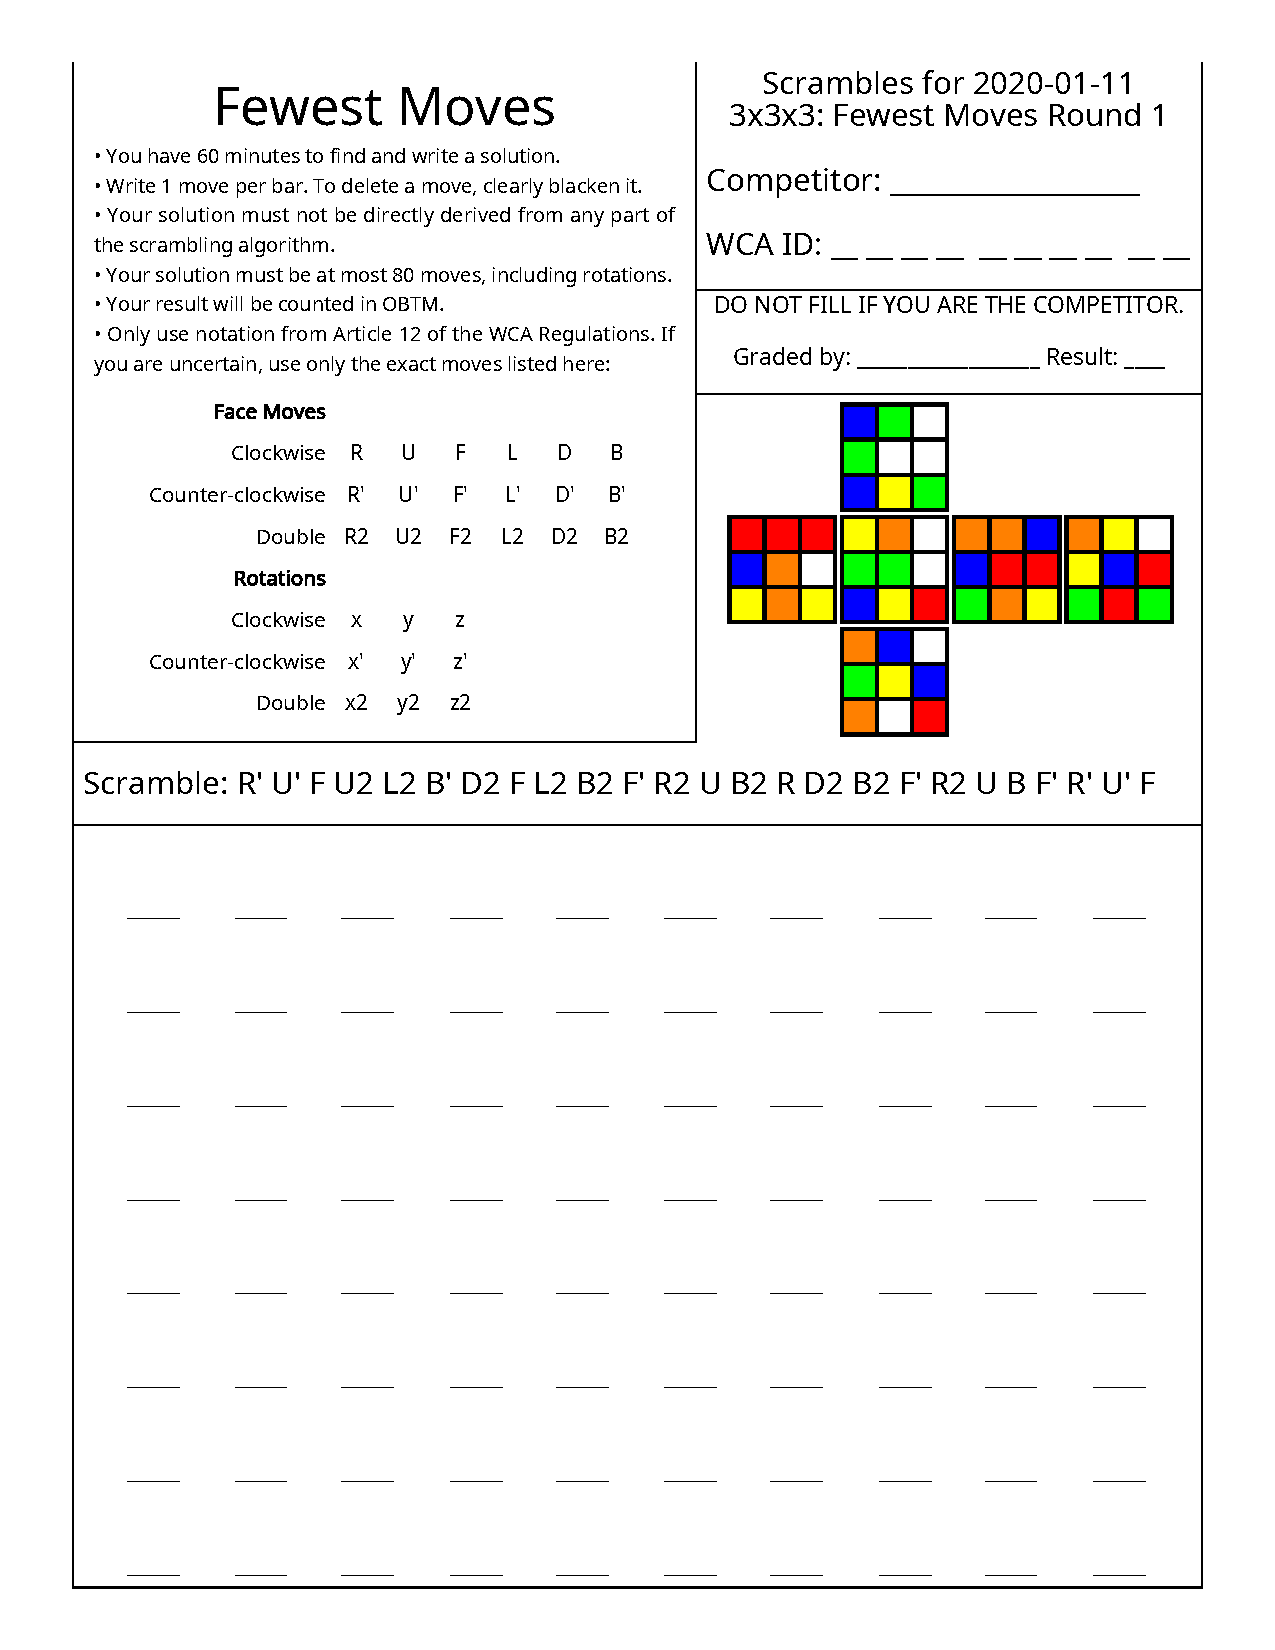
\includegraphics[scale=0.7]{img/example.pdf}
\end{center}
\caption{Example of official scramble sheet.}
\end{figure}

In order to enforce the last rule, since 2016 scrambles are generated so that they begin and end with the sequence \m{R\p} \m U \m F.

The best results ever achieved in competition are 16 moves for the single shortest solution and 22.00 moves for the average of three attempts, while the current world champions (Firstian Fushada, Indonesia and Christopher Chi, USA) got their title with an average of 25.33 moves.

\section*{Goal of this tutorial}

The goal of this tutorial is to summarize the best known techniques that lead to good results in fewest moves solving. In some cases the explanation will be detailed and enriched with examples, while in some other I will only provide a synthetic explanation and suggest other resources for further study.

\chapter{Think outside the box}

Whatever your main method is, forcing yourself to only use that method is the worst thing you can do in FMC. \textbf{You should never restrict yourself to only one method}, but try to exploit every situation.

For example, suppose you have built a 2x2x3 block; now you have many possibilities: you can place the last ``cross'' edge and finish the F2L (CFOP), you can orient edges (Petrus) or try to build more blocks freely (FreeFOP, Heise) and so on. Any of this methods may lead to a good solution, so the best thing to do is to \textbf{try to use them all} (or most of them at least).

The best way to open your mind and learn how to think outside the box is, maybe a little paradoxically, to \textbf{get into many ``boxes''}, that is to learn many methods. Here I will briefly describe those that are, in my opinion, the most useful methods for FMC, without talking about their development history nor their pro/cons in speedsolving. For each of these methods I will provide a link to an online tutorial, but I suggest you look for more information about them online, for example on speedsolving.com. The
\href{https://www.speedsolving.com/forum/threads/beginners-guide-to-choosing-a-speedsolving-method.43471/}{\emph{Beginner's Guide to Choosing a Speedsolving Method}}\footnote{\url{https://www.speedsolving.com/forum/threads/beginners-guide-to-choosing-a-speedsolving-method.43471/}} on the speedsolving forum, although mainly intended for speedsolving, is a good starting point for getting more information about the 4 most commonly used methods (CFOP, Roux, ZZ and Petrus).

\section{Petrus}

Petrus' steps are the following:
\begin{enumerate}
\item Build a 2x2x2 block.
\item Expand the 2x2x2 block to a 2x2x3 block.
\item Orient edges.
\item Complete the first 2 layers (F2L).
\item Solve the last layer (originally divided into 3 steps).
\end{enumerate}

Having a good \textbf{blockbuilding}\footnote{``Blockbuilding'' or ``block-building'' is the technique that consists of making blocks of pieces and then joining them together. It is often seen in opposition to the way of building the F2L used in CFOP (see below), but this can also be seen as a kind of blockbuilding. A more suitable contrast is given by comparing it to other techniques, such as edge orientation (Petrus, ZZ), ``Corners First'' solving, using algorithms or commutators. All of these techniques are explained in this book.} skill is mandatory if you want to get good at FMC, and practicing Petrus is the best way to acquire it. To learn how to solve steps 1 and 2 efficiently, you need to think and try to explore different ways of building blocks every time; it is also very useful to study \textbf{reconstructions of expert cubers' solves}. For the first step it is also helpful to compare your solutions with the optimal ones, given by an optimal solver\footnote{For example \href{https://www.speedsolving.com/forum/threads/harcs-jarcs-replacement-cube-solver.63241/}{HARCS}, freely available online: \url{https://www.speedsolving.com/forum/threads/harcs-jarcs-replacement-cube-solver.63241/}}, since for an expert it should be (almost) always possible to find an optimal 2x2x2 block.

Step 3 teaches you how to recognize an edge's orientation regardless its position in the cube. This is another important skill, since flipped edges are one of the worst thing you may come across during an FMC solve. For this step, as well as for step 4, ZZ may be a better teacher than Petrus.

You don't have to learn every algorithm for solving the last layer (the same is true for other methods too). In the next chapter I will explain in detail how you should proceed. For now it is enough to be aware that the ``last layer'' step usually is not included in Fewest Moves solutions.

Lars Petrus Website: \url{http://lar5.com/cube/}.

\section{Roux}

\begin{enumerate}
\item Build a 3x2x1 block.
\item Build another 3x2x1 block, opposite to the first one.
\item Solve the corners of the last layer, without necessarily preserving the M layer (CMLL).
\item Solve the last six edges (LSE).
\end{enumerate}

Petrus is an excellent method to learn blockbuilding, but forcing yourself to only use Petrus is still wrong: learning also Roux (especially the first 2 steps) will make your skill in some sense more complete. Also for this method it will be useful to study solutions of more expert cubers.

For step 3 it still stands what was said about last layer algorithms, while step 4 is to be avoided like plague (at least, avoid solving it in the ``standard'' way, i.e. using only M and U moves): remember that every inner layer move, like M, is worth 2 moves in standard metric!

Waffle's Roux Tutorial: \url{http://wafflelikescubes.webs.com/}.

Kian Mansour's Roux Tutorial: \url{https://sites.google.com/view/kianroux/home}.

\section{ZZ}
\begin{enumerate}
\item EOLine (orienting all edges and placing DF and DB, leaving the cube to be possibly solved moving only the R, L and U layers).
\item F2L.
\item Last Layer.
\end{enumerate}

As mentioned earlier, recognizing and solving edge orientation is a very useful skill and ZZ is surely the best way to learn it. At first sight ``orienting edges'' can be hard, because it is a more abstract concept than ``building blocks'', but don't panic, it gets way easier with practice!

Step 2 is more or less the same as Petrus' step 4, but you have to build the blocks on both R and L side at the same time\footnote{For speedsolving, it may be better to solve one block at the time, since it is usually more ergonomic. But this is not the case for FMC, as efficiency (i.e. number of moves) is the only thing that matters!}. This is also going to improve your blockbuilding skills.

\section{CFOP (Fridrich) and FreeFOP}
In classic CFOP the steps are the following:
\begin{enumerate}
\item Cross (4 edges on the same side).
\item 4 corner/edge pair insertions.
\item OLL (Orient Last Layer).
\item PLL (Permute Last Layer).
\end{enumerate}

Classic CFOP is \textbf{not} considered a good method for FMC, but in some situations it is useful to know different ways to insert a corner/edge pair.

In FreeFOP, the first two steps are replaced by a ``free'' blockbuilding F2L.

Anyways, I strongly advise against solving the last layer with OLL + PLL, unless you get to skip one of the two steps.

Badmephisto's Tutorial: \url{http://badmephisto.com/}.

\section{Keyhole F2L}

Keyhole is not really a method to solve the cube, but a technique to solve the first two layers. It is considerate an intermediate method between “Layer by Layer” and CFOP. The steps are the following:
\begin{enumerate}
\item Cross.
\item Place 3 first layer corners.
\item Insert 3 middle layer edges, using the ``free'' corner slot.
\item Insert the last corner/edge pair, as in CFOP or as in LBL.
\end{enumerate}

To improve efficiency you should replace the first two steps with blockbuilding and place a few middle layer edges in the meantime. A variation consists in solving the cross and 3 middle layer edges, and then placing 3 first layer corners using the ``free'' edge slot.

Despite its simplicity, this method can be very useful in FMC.

\section{Heise}
\begin{enumerate}
\item Build four 2x2x1 ``squares'' (all sharing one colour).
\item Match the squares and orient edges.
\item Solve the remaining 5 edges and 2 corners.
\item Solve the last 3 corners using a commutator.
\end{enumerate}

If you decided not to follow the experts' advice and use only one method for FMC, Heise would be a good choice. This method alone can lead to and average of fewer than 40 moves for linear\footnote{As in ``linear'' FMC, that is without trying different possibilities and/or cancelling or undoing moves.} solves. It is an extreme method, but also extremely efficient.

The first two steps are a strange but efficient way of building an F2L-1\footnote{With ``F2L-1'' I mean an F2L minus a coner/edge pair.} and orient all edges. The ``don't restrict yourself'' and ``exploit different situations'' concepts is perfectly applied, allowing one to solve the blocks in whatever the best way is.

The third step is complex, but it is a more efficient alternative to finishing the first two layers and then solving the last layer using algorithms. Practicing it will give you the ability to build and move around blocks when you are limited by the quantity of blocks already built (and this is the reason why this step is so difficult).

For the last step you will need commutators; it allows, in an FMC solve, to use insertions (both these techniques will be explained in the next chapter).

Heise method's page on Ryan Heise's website: \url{http://www.ryanheise.com/cube/heise_method.html}. There you can find not only a detailed explanation of his method, but also other useful information (see for example the \href{http://www.ryanheise.com/cube/fundamental_techniques.html}{\emph{Fundamental Techniques} page}).

\section{What and how to learn}
Obviously, getting fast with all of the methods described is not your goal. Doing some speedsolves may help seeing some things faster and is fun, but \textbf{we don't care about speed}. Since our goal is to solve the cube with the fewest moves possible, you should try to be efficient. It is also essential to be \textbf{color neutral}\footnote{Being able to solve the cube by starting with any ``colour''; for example, starting from any cross in CFOP or from any of the 8 possible 2x2x2 blocks in Petrus.} and it can be helpful trying to work with \textbf{``Non Matching Blocks''}\footnote{Sometimes also called ``Pseudo Blocks'', especially in FMC. It is a useful technique in Roux, ZZ and Heise, but it can be used in other methods as well. It consists of building blocks that are different from the ones you should build if you are following the method, but that can be placed in the same ``slots''. For example, in Roux, the second 3x2x1 block can be any of the 4 that can be built on the side opposed to the first one. This technique is very powerful if combined with premoves, that will be explained in Chapter 3.}.

But the main difference between speedsolving and fewest moves solving is that in FMC you can \textbf{try different possibilities}. If in Petrus, for example, you are left with 6 ``bad'' edges after a 2x2x3, you can try to build a different block from scratch or to slightly modify the construction of the block you have found to improve your situation\footnote{Trying to influence a later step while solving the current one is a good habit, which will be discussed again later.}.

Here is some piece of advice for some of the methods described.

\subsection{Petrus}
\begin{itemize}
\item After completing a 2x2x2 block, you can expand it in \textbf{3 different directions}. Make sure to consider all of them!
\item Try to build a 2x2x3 directly, instead of going through the 2x2x2 step.
\item Try using Non Matching Blocks in step 4.
\item In step 4 again, try influencing the last layer to get an easier case (even ``Heise style'').
\end{itemize}

\subsection{Roux}
\begin{itemize}
\item Try to build the two blocks at the same time.
\item Try Non Matching Blocks.
\item Influence the CMLL while finishing the second block, and the LSE during the CMLL.
\end{itemize}

\subsection{ZZ}
\begin{itemize}
\item After edge orientation, building the ``Line'' isn't always a good idea: try blockbuilding directly (without breaking the EO!). The difference between solving the line first and then the right and left blocks is comparable to the difference between doing CFOP with cross + F2L pairs and doing FreeFOP.
\item Once you have oriented the edges, you have reduced the cube to be solved moving only the R, L ,U and D layers: you can build the F2L on any of these sides.
\item As in Petrus and Roux, try using Non Matching Blocks and influencing the last layer while building the F2L.
\end{itemize}

\subsection{CFOP/FreeFOP}
\begin{itemize}
\item \textbf{FreeFOP is better than CFOP}, at least because CFOP is a special case of FreeFOP, by definition. Try at least to build and \textbf{XCross}\footnote{Cross and first pair, built at the same time. It can also be seen as a 2x2x2 block + 2 edges.}.
\item Try to influence the last layer edges' orientation, avoid the ``4 edges flipped'' cases; some ZBF2L algorithms can be useful, but instead of learning them by heart try to \textbf{study them to understand how they work}.
\item Some optimal pair insertion algorithms are not well known (for example \m{F2 U R U\ps R\ps F2}): study them, again trying to understand them rather than learning them by heart.
\item Try \textbf{``multislotting''}, that is inserting more pairs at the same time. The easiest case is when you use a D-layer move as setup, for example \m{D R U R\ps D\p}. There are algorithms for this technique available online, but I suggest trying in a ``free'' way: for example, look at how I have inserted the second, third and fourth pair in this solve: \url{https://www.speedsolving.com/forum/threads/the-3x3x3-example-solve-thread.14345/page-238#post-1013053}.
\end{itemize}

\chapter{How to proceed during a solve}

To quote Per Kristen Fredlund, the general way to proceed is the following\footnote{\url{http://www.speedsolving.com/forum/threads/fewest-moves-tips-and-techniques.1566/##post-16209}}:

\begin{center}“\emph{Think of it more like so: solve the cube in 2 stages where stage 1 solves as many pieces as possible as efficiently as possible (i.e.: make a good skeleton\footnote{A partial solution, where only a few pieces (usually from 2 to 6) are left to be solved.}). The second step is fixing the unsolved pieces, typically by inserting algorithms into the skeleton\footnote{Technique that allows to solve a few pieces by inserting moves somewhere earlier in the solve. It will be explained soon, be patient!}''.}
\end{center}

This is the general approach, but you don't need to use it every time: sometimes you can find a very short solution by, for example, solving the F2L with blockbuilding and then finishing the last layer with an algorithm. There are also different ways to proceed, two of which will be explained in Chapter 4.

If this description seems too generic, it is because it can't be differently: there isn't a standard method that allows you to always get good results, \textbf{you should always try as many strategies as you can}, so that you don't miss any chance.

Here I will describe some basic techniques used in FMC solves. You have already learnt some of them by practicing the methods described in the previous chapter, while you will need to study some other. Some will be explained in detail, some other will be only mentioned and other tutorials will be linked for a more complete study.

\section{Blockbuilding}

Blockbuilding is probably the most important technique in FMC. It is a simple concept, but it requires a lot of practice to be mastered. Practicing blockbuilding-based methods (Petrus, Roux, Heise and ZZ), in the ways described above, is the most direct way to improve at blockbuilding.

Here I will list some fundamental techniques that can come in handy; the first ones are taken from Ryan Heise's website (\url{www.ryanheise.com/cube}), which is full of examples: look them up!

\subsection{Align then join}
\label{align-join}
Source: \url{http://www.ryanheise.com/cube/align_join.html}\bigskip

Basic technique: to build a corner/edge pair, the simplest kind of block, you have to align them first, making them joinable by a single move, and then join them with that move.

This concept can be applied, in a more general meaning, to the case of bigger blocks, for example when you want to match a pair and 2x2x1 square to get a 3x2x1.

All of this may look trivial, and in some way it is; the important thing to learn is to \textbf{recognize when two pieces are aligned} and can be therefore joined with one move. This way you will be able to realize in advance whether a certain move will join 2 pieces.

\bigskip
\begin{tabular}{|p{0.91\textwidth}|}
\hline
\textbf{Align then Join - Example}\\
\hline
Scramble: \m{F U\ps D2 L D L2 D F R2 B U2 R2 D L2 D L2 D R2 U\ps L2 F2}\\
\hline
\begin{minipage}[l]{0.650\textwidth}
\m{L2}\comment{Align}\\
\m{U2}\comment{Join}
\end{minipage}
\begin{minipage}[c]{0.25\textwidth}
\includesvg{img/align-join}
\end{minipage}\\
\hline
\emph{See on }\href{https://alg.cubing.net/?alg=L2_\%2F\%2FAlign\%0AU2_\%2F\%2FJoin&setup=F_U-_D2_L_D_L2_D_F_R2_B_U2_R2_D_L2_D_L2_D_R2_U-_L2_F2}{\emph{alg.cubing.net}}\\
\hline
\end{tabular}
\bigskip

In the example above, two pairs are already built. The sequence \m{L2 U2} pairs up the blue-red edge with the blue-red-yellow corner.

\subsection{Move it out of the way}
Source: \url{http://www.ryanheise.com/cube/move_it_out_of_the_way.html}\bigskip

It can happen that we want to build a block, but the move required to build it breaks other blocks, or moves away pieces that we don't want to move. One of the ways to bypass this problem is to move away such pieces first, saving them from the breaking move, and then, if necessary, put them back together once the move has been performed.

\bigskip
\begin{tabular}{|p{0.91\textwidth}|}
\hline
\textbf{Move it out of the Way - Example}\\
\hline
Scramble: \m{F R2 B D2 F D2 L2 B2 F\ps D2 F\ps L B U\ps F2 U2 L2 U B R2 F}\\
\hline
\begin{minipage}[l]{0.650\textwidth}
\m{U2 R2 D R2}\comment{2x2x1 square}\\
\m{U\p}\comment{Move the red-white-blue pair out of the way!}\\
\m{F\ps D\p}\comment{Expand the square to a 2x2x2 block}
\end{minipage}
\begin{minipage}[c]{0.25\textwidth}
\includesvg{img/move-way}
\end{minipage}\\
\hline
\emph{See on }\href{https://alg.cubing.net/?setup=F_R2_B_D2_F_D2_L2_B2_F-_D2_F-_L_B_U-_F2_U2_L2_U_B_R2_F&alg=U2_R2_D_R2_\%2F\%2F2x2x1_square\%0AU-_\%2F\%2FMove_the_red\%26\%2345\%3Bwhite\%26\%2345\%3Bblue_pair_out_of_the_way\%0AF-_D-_\%2F\%2FExpand_the_square_to_a_2x2x2_block}{\emph{alg.cubing.net}}\\
\hline
\end{tabular}
\bigskip

If we did \m{F\ps D\p} right after building the 2x2x1 block we would still get the same 2x2x2 block, but we would break the red-white-blue pair. Notice however that in this case ``moving it out of the way'' doesn't seem to be the best idea: in the process of saving that pair, we are breaking the yellow-orange-blue one!

\subsection{Destroy and restore}

Source: \url{http://www.ryanheise.com/cube/destroy_restore.html}\bigskip

Another way to solve this problem is to temporarily break some blocks and join them back later, using the ``move it out of the way'' technique.

A basic example is given by applying the ``scramble'' \m{R U R\ps U\p}.

\begin{center}
\includesvg{img/sexy}
\end{center}

Let's ignore the last layer and pretend not to know that \m{U R U\ps R\p} obviously solves the cube. Looking at the first two layers only, we see that \m{R\p} places the yellow-green-red pair next to the other pieces in the front layer, but breaks part of the F2L already built. We can use “Destroy and Restore” this way:

\bigskip
\m{R\p}\comment{``Destroy''}

\m{F}\comment{``Move it out of the Way''}

\m R\comment{``Restore''}

\m{F\p}\comment{Put back the pieces moved away with \m F}

\subsection{Keyhole}

We talked about it earlier as a standalone method, but keyhole can be considered a particular strategy to build blocks. This  technique consists in exploiting unsolved parts of the cube to solve some other pieces. After some good Keyhole F2L practice you shouldn't need any example to understand what I mean, but I'll leave here a Keyhole solve anyways.

\bigskip
\begin{tabular}{|p{0.91\textwidth}|}
\hline
\textbf{Example (adapted from a solve by Edoardo Disarò)}\\
\hline
Scramble: \m{U\ps R\ps L F\ps B U2 R2 B2 L\ps B R D F2 D2 L2 F2 D\ps R2 F2}\\
\hline
\begin{minipage}[l]{0.650\textwidth}
\m{F\ps L\p}\comment{Layer minus one corner}\\
\m{F2 L\ps B\ps L}\comment{Keyhole}\\
\m{F U\ps B U}\comment{Keyhole, accidentally solving the last corner}\\
\m{F\ps R\ps B2 R}\comment{Keyhole}\\
\m{F B L B L\p}\comment{F2L}\\
\m{B\p}\comment{LL}
\end{minipage}
\begin{minipage}[c]{0.25\textwidth}
\includesvg{img/keyhole-example}
\end{minipage}\\
\hline
\emph{See on }\href{https://alg.cubing.net/?setup=U-_R-_L_F-_B_U2_R2_B2_L-_B_R_D_F2_D2_L2_F2_D-_R2_F2&alg=F-_L-_\%2F\%2FLayer_minus_one_corner\%0AF2_L-_B-_L_\%2F\%2FKeyhole\%0AF_U-_B_U_\%2F\%2FKeyhole,_accidentally_solving_the_last_corner\%0AF-_R-_B2_R_\%2F\%2FKeyhole\%0AF_B_L_B_L-_\%2F\%2FF2L\%0AB-_\%2F\%2FLL}{\emph{alg.cubing.net}}\\
\hline
\end{tabular}
\bigskip

\subsection{One move, two goals}

It is often possible to use only one move to build two blocks or, in general, to ``get two things done''. An example will make this clearer.\footnote{Clarification: the solution was found independently by both, not in cooperation}

\bigskip
\begin{tabular}{|p{0.91\textwidth}|}
\hline
\textbf{Example (by Mirek Goljan and Guus Razoux-Schultz})\\
\hline
Scramble: \m{D U\ps F2 U\ps R\ps F R2 B D\ps B R F B\ps U R\ps D2 L\ps R2 F2 B\ps U\ps B D B2 F2 U L F U\ps B2}\\
\hline
\begin{minipage}[l]{0.650\textwidth}
\m{L U\ps {\color{red}F2} D\p} \comment{2x2x2 (4/4)}\\
\m{U2 B R2 B} \comment{Pseudo F2L-1 (4/8)}\\
\m{F\ps * U F R U2 R\p} \comment{Pseudo F2L (6/14)}\\
\m{U2 R2} \comment{All but 3 corners (2/16)}\\
\m{* = B\ps U F2 U\ps B U F2 U\p} \comment{Last 3 corners (3/19)}
\end{minipage}
\begin{minipage}[c]{0.25\textwidth}
\includesvg{img/mirek-guus}
\end{minipage}\\
\hline
Solution: \m{L U\ps F2 D\ps U2 B R2 F\ps U F2 U\ps B U F\ps R U2 R\ps U2 R2} (19)\\
\hline
\emph{See on }\href{https://alg.cubing.net/?setup=D_U-_F2_U-_R-_F_R2_B_D-_B_R_F_B-_U_R-_D2_L-_R2_F2_B-_U-_B_D_B2_F2_U_L_F_U-_B2&alg=L_U-_F2_D-_\%2F\%2F2x2x2_(4\%2F4)\%0AU2_B_R2_B_\%2F\%2FPseudo_F2L\%26\%2345\%3B1_(4\%2F8)\%0AF-_(B-_U_F2_U-_B_U_F2_U-)_U_F_R_U2_R-_\%2F\%2FPseudo_F2L_(6\%2F14)\%0AU2_R2_\%2F\%2FAll_but_3_corners_(2\%2F16)}{\emph{alg.cubing.net}}\\
\hline
\end{tabular}
\bigskip

If you don't know about insertions yet, ignore the last line. In fact the only line we are concerned with is the first one, especially the red \m{F2} move: notice how that single move builds the 2x2x1 block in DF and places the orange-green edge at the same time, which allows to build the 2x2x2 with the next move.

Situations like this may arise without forcing them, but it useful to learn to recognize them, in case they don't.

\subsection{Influence later steps}

We have already (quickly) talked about influencing the LL step while finishing the F2L\footnote{Notable examples are ZBLS (sometimes less properly called ZBF2L) and Winter Variation, but there are many more: look them up!}. This idea also applies to blockbuilding: it is often better to build a block sub-optimally\footnote{``Sub-optimal'' (or ``suboptimal'', without the -) refers to a solution (complete or partial) that uses more moves than the best possible one.}, or to add some ``unnecessary'' moves to have a better continuation, blockbuilding or else (i.e., edge orientation).

For example, consider the following scramble.

\bigskip
\begin{tabular}{|p{0.91\textwidth}|}
\hline
\textbf{Influence Later Steps - Example}\\
\hline
Scramble: \m{L2 D2 U R2 F2 D2 B2 U\ps R2 B2 U B U F D B2 U L D\ps R\ps F}\\
\hline
\begin{minipage}[l]{0.650\textwidth}
\m{L2 {\color{red}B} R B}\comment{Two 2x2x1 blocks}
\end{minipage}
\begin{minipage}[c]{0.25\textwidth}
\includesvg{img/influence-steps}
\end{minipage}\\
\hline
\emph{See on }\href{https://alg.cubing.net/?setup=L2_D2_U_R2_F2_D2_B2_U-_R2_B2_U_B_U_F_D_B2_U_L_D-_R-_F&alg=L2_B_R_B_\%2F\%2FTwo_2x2x1_blocks}{\emph{alg.cubing.net}}\\
\hline
\end{tabular}
\bigskip

As you can see, the sequence \m{L2 R B} builds the red-blue-white square, but if you add just one move (the red \m{B}) the square become 2.

\subsection{Pay attention to EO}
\label{EO_attention}

Here EO is the common shortcut for Edge Orientation.

Someone may have noticed, while studying different methods, that “Edges Orientation” is a recurring step. As said before, \textbf{the more bad edges there are, the harder things will be}. Orienting edges at the end is usually not efficient. Orienting them first, as in ZZ, is convenient, but it can be limiting for the blockbuilding phase.

One of the best things to do is trying to solve, at least partially, edges orientation during the blockbuilding step. Experience with methods such as ZZ and Petrus can lead to being able to easily spot if an edge will be correctly oriented after some moves. If you don't have this ability yet, remember that in FMC solves you can go back and modify your solution every time you wish: if you have troubles with EO, try going back and add/change some moves to see if things get better (see also Section \ref{goback}).

However, don't dismiss the ``EO first approach'' too quickly: notable cubers such as João Pedro Batista Ribeiro Costa (2015 World Champion) and Grzegorz Łuczyna (2010 European Champion) almost always start with edge orientation and other like Sébastien Auroux (2011 World Champion) and myself do it very often. For more details and examples see section \ref{eo}.

\subsection{Which block should I build?}

The golden rule is to exploit different situations: a 2x2x2 block, a 3x2x1, two 2x2x1 squares and many other kind of blocks can be a good start. Try out every possibility.

Two possible approaches are:
\begin{enumerate}
\item Try completing big blocks, like a 2x2x3 or a F2L-1.
\item Proceed in small steps, building many small blocks and joining them at the end.
\end{enumerate}

Erik Jernqvist proposes the following number of moves as good starts\footnote{Taken from this post on speedsolving.com: \url{https://www.speedsolving.com/threads/the-fmc-thread.13599/page-42\#post-614593}. Obviously, what ``good start'' means depends on your level. The given move counts are to be considered a good goal for someone who wants to become an expert. If you are not this good yet you can go on with less efficient blocks. Don't waste too much time looking for a good start: it's the final result that counts!}:

\bigskip
\begin{center}
\begin{tabular}{|l|c|}
\hline
Type of Blocks & Number of Moves\\
\hline
2x2x1 square + corner/edge pair & 3\\
\hline
2x2x2 block & 4\\
\hline
Two 2x2x1 squares & 5\\
\hline
2x2x3 block & 9\\
\hline
F2L-1 & 14\\
\hline
F2L & 17\\
\hline
\end{tabular}
\end{center}

Personally, I think these are good estimates, especially for the first 3 cases. But you always have to remember that \textbf{how good a start is depends on the possible continuations}. If you build an F2L-1 in 12 moves, but you have 4 bad edges, one of which is the last F2L edge flipped in place, you may have to throw it away. On the other hand, a 2x2x3 in 12 moves with all edges oriented can be a better alternative. Obviously EO is not the only thing you have to consider, but it is one of the most important.

Another rule is: \textbf{never\footnote{But a more important rule is: never say never!} complete the F2L without influencing the last layer}. The reason is simple: a bad last layer can require many moves, no matter how many algorithms you know, and a completely built F2L gives a little freedom to manipulate the cube. On the other hand, \textbf{an F2L-1 is a good partial goal}, because it leaves you more freedom, despite the many pieces already placed.

\subsection{Ready-made blocks: how to deal with them?}
\label{ready-made}

It can happen that you find some blocks already built after scrambling the cube, or that with the first moves you unintentionally build some more blocks (mostly corner/edge pairs). In this cases it is preferable to exploit those blocks rather than giving them and up and going on your own way. How? There are three ways:

\begin{enumerate}
\item Expand / match the ready-made blocks first; the obvious thing to do.
\item Expand / match the ready-made blocks, but \textbf{watching other pieces too} and trying to build other blocks at the same time; this is usually the best thing to do.
\item Don't expand the ready-made blocks, but try to make new ones, possibly saving the others.
\end{enumerate}

Moreover, it is very important, but terribly difficult, to \textbf{understand when it is not worth to save a block}, and you should break it to make new ones. Personally, I find it very hard to ``give up'' and ``throw away'' a block, but I realize this often causes troubles, especially in time management.

\subsection{Tricks to get fast and advanced techniques}

``Getting fast'' is not to be intended as in speedsolving, but as ``finding faster a good blockbuilding start\footnote{A ``start'' can be a 2x2x2, a 3x2x1, some smaller blocks or, in some cases, a 2x2x3; in general, anything from the first 2 to the first 7 moves.}''. Being fast at finding a good start is very important, because it saves time (one hour isn't that long!) and you should try to explore, or at least to notice, every promising start.

The simplest kind of block is the corner/edge pair, or 2x1x1 block. There will probably be one already made in a scramble, without making any move. If there is one (or more than one), you can deal with it in one of the ways described in the previous section \ref{ready-made}. If there isn't any, you should learn how to recognize at sight pairs that can be made with one move (see \ref{align-join} ``Align Then Join''). If you are not fast at recognizing them yet, or if you want to avoid some effort\footnote{Since you need to keep thinking for an hour, avoiding unnecessary mental effort is a good habit.}, you can use the ``Brute Force'' strategy: try all possible moves, starting with \m U, \m{U2}, \m{U\p}, then \m R, \m{R2}, \m{R\p}, and so on, checking after each move if you did build a pair.

A more advanced technique, more useful but requiring more thinking, consists in checking every possible 2x2x2 (there are 8 of them). You can do it this way: \textbf{for each corner, look for its three matching edges} and try to see which way you can join them to make that 2x2x2 block. Try not to make any ``test'' moves, so that you can do the same for the other corners without re-scrambling. Usually, if I see a very bad 2x2x2 block (one that requires too many moves) I just ignore it and go on. This technique, besides enabling you to find, most of times, an optimal 2x2x2 block (which is usually a good starting point), gives you an idea of where every piece is on the cube.

Another reason why I suggest trying to ``see'' every move for making the 2x2x2 without performing them is that to get faster and better at blockbuilding it is useful to be able to ``calculate''\footnote{The word ``calculate'' should be intended as in chess: a player is said to ``calculate'' 6, 7 or 8 moves if he can think of the possible moves and counter-moves for a total of 6, 7 or 8 moves.} pieces' movements without seeing them. Alexander Lau (2014 Rubik's Cube European Champion and Roux method master) is able, in the 15 seconds given to inspect the cube before a speedsolve, to plan a whole 3x2x1 block (Roux first step). His planning is so accurate that while solving this block he can look-ahead\footnote{In speedsolving, ``look-ahead'' (with or without the -) is the ability to think about later step while you are solving another one.} and (partially) plan the second block.

You can train your planning ability with this game: ask a friend to scramble your cube with 3 moves and then try to find those 3 moves\footnote{You can choose between HTM, QTM or STM, but agree on which metric to use first!} (it should be easy). Then try with 4 moves, and so on. Depending on your level, you may find it difficult once you reach 6, 7 or 8 moves. If you get without problem to 9 or 10 moves, congratulations!

\section{Find a good skeleton}

Once you have reached good point (for example an F2L-1) with blockbuilding, it is hard to go on with the techniques just described. Your goal now is to find a so-called ``skeleton'', i.e. a partial solution that only leaves a few pieces unsolved. The best situation is the one with 3 corners unsolved, where the pieces form a 3-cycle\footnote{A 3-cycle is a cycle of 3 pieces. For example, the A and U perm PLL cases are 3-cycles, as well as the algorithm \m{L F R F\ps L\ps F R\ps F\p} (Niklas).}, but also 4 or 5 corners or 3 edges can be good, depending on how many moves you need to build the skeleton.

What should we do then, if the blockbuilding techniques we have seen are difficult to use without destroying what we have just built? Heise is an excellent starting point. And I mean both the method and the website: step 3 is accurately described, in particular the ``Two Pairs Approach'': see \url{http://www.ryanheise.com/cube/two_pairs.html}.

Heise's step 3 requires not only an F2L-1, but also all edges to be oriented. If they are not, you can:
\begin{enumerate}
\item orient them now; usually not recommended, unless it takes very few moves;
\item modfy the steps you have already solved, to get all edges oriented at the end;
\item orient them while finishing your skeleton.
\end{enumerate}

To sum it up, the possible approaches to get a skeleton are many and the best way to practice in this case (and always a good habit) is to look online (for example in websites hosting online competitions or on speedolving forums) for expert FMCers' solves; most of times, they build a skeleton.

Some deliberate practice can also be helpful: on qqTimer (\url{http://www.qqtimer.net/}) you can choose the scramble type 3x3x3 subsets $\rightarrow$ last slot + last layer.

You obviously don't have to build an F2L-1 before completing your skeleton, but is often the easiest way. In any case, try to save small blocks (pairs or 2x2x1 squares) made by LL pieces, if some of them happen to get built.

\section{Commutators}

According to speedsolving's definition\footnote{\url{http://www.speedsolving.com/wiki/index.php/Commutator}}, a commutator is a sequence of moves of the form

\begin{center}
\m{A B A\ps B\p}
\end{center}

where \m A and \m B are move sequences and \m{X\p} is the inverse sequence of \m X\footnote{For example, the inverse of \m{U R} is \m{R\ps U\p}, not \m{U\ps R\p} or \m{R U}!}. Such a commutator can be written in compact notation as

\begin{center}
\m{[A, B]}
\end{center}

The name and notation for commutators come from Mathematics, in particular from Group Theory. See \url{https://en.wikipedia.org/wiki/Commutator}.

For example taking \m{A} = \m{R} and \m{B} = \m{U} realizes the ``sexy move'' as a commutator:
\begin{center}
\m{[R, U]} = \m{R U R\ps U\p}
\end{center}

Taking instead \m A = \m R and \m B = \m{U\ps L\ps U} gives the ``Niklas'':

\begin{center}
\m{[R, U\ps L\ps U]} = \m{R U\ps L\ps U R\ps U\ps L U}
\end{center}

Often, in practice, ``commutator'' is used as ``commutator that solves a 3-cycle''. So for example the ``sexy move'' is not usually regarded as a commutator, while the ``Niklas'' is. In what follows, we will use the word ``commutator'' this meaning too.

In contrast with blockbuilding, that solves a lot pieces but heavily influencing the rest of the cube, commutators solve fewer pieces leaving all the others where they were. Therefore, together with blockbuilding and insertions (which we will see in the next section), commutators are the basis for a good FMC solve.

\subsection{Corner commutators}

Corner commutators are the most useful kind of commutators in FMC. We have already seen the ``Niklas'' as a commutator. Also the A perm PLL case \m{R2 B2 R F R\ps B2 R F\ps R} is (almost) a commutator:

\begin{center}
\m{R2 B2 R F R\ps B2 R F\ps R} = \m{R2 [B2, R F R\p] R2}
\end{center}

where we have cancelled\footnote{In a sequence of moves, we say that one or more moves \emph{cancel} if there are consecutive moves that can be merged together (as in our example \m{R\ps R2} = \m R) or that are one inverse to the other (such as \m{L L\p}). For example, if our F2L ends with \dots\m{U R2 F\p}, and we want to use the algorithm \m{F R U R\ps U\ps F\p}, 3 moves cancel:
\dots\m{U R2 F F\ps R U R\ps U\ps F\p} = \m{U R\ps U R\ps U\ps F\p}.} the sequence \m{R\ps R2} to \m R.

The three corners to be permuted need not be on the same layer: \m{[L D\ps L\p, U2]} = \m{L D\ps L\ps U2 L D L\ps U2} is also corner 3-cycle!

To learn all kinds of corner commutator (which I will \emph{not} explain in this tutorial) I advise looking up \href{https://www.speedsolving.com/forum/threads/bh-tutorial.12268/}{Brian Yu's tutorial} on speedsolving.com\footnote{\url{https://www.speedsolving.com/forum/threads/bh-tutorial.12268/}}, since it is very well made. It used to consist of both a written part and some videos, but the videos are unfortunately not available anymore.

For FMC you only need to know ``pure'' 8 moves commutators. For example, the Niklas is a pure commutator, while the A perm is not. Take a look at A9s and other cases if you want, but, as we will see when talking about insertions, you will almost never\footnote{Even in this case there are exceptions: see for example this post by Tomoaki Okayama and the following discussion: \url{https://www.speedsolving.com/threads/the-fmc-thread.13599/page-21##post-440873}.} need them in FMC.

On rare occasions, 10 moves ``sledge insertion'' corner commutators such as \m{[R\ps F R F\p, D2]} may be useful, because they may cancel many more moves than the standard 8 moves commutators.

\subsection{Edge commutators}

Once you have learned corner commutators, it should not be hard to understand how edge commutators work, especially the ones like

\begin{center}
\m{[U R U\p, M\p]} = \m{U R U\ps M\ps U R\ps U\ps M}
\end{center}

Sadly, commutators like this only occasionally give a good result, because they use M layer moves, which are actually two moves in our metric.

The edge commutator \emph{everyone should know} is:

\begin{center}
\m{[M\p, U2]} = \m{M\ps U2 M U2}
\end{center}

Which is also very useful with some setup move, for example:

\begin{center}
\m{[U: [M\p, U2]]\footnote{The notation \m{[A: B]} = \m{A B A\p} stands for a \emph{conjugate}. The sequence \m A is usually called ``setup moves''.}} = \m{U M\ps U2 M U2 U\p} = \m{U M\ps U2 M U}
\end{center}

Remember that in official competitions you can't write a inner layer moves, so the \m{[M\p, U2]} commutator becomes:

\begin{center}
\m{M\ps U2 M U2} = \m{R\ps L x U2 R L\ps x\ps U2} = \m{R\ps L F2 R L\ps U2}
\end{center}

Notice how the first two moves (\m{R\ps L}) can be swapped. This is true for every pair of parallel (i.e. opposite) moves.

Another thing you need to notice is that the first two moves don't affect any of the 3 edges we want to cycle: \m{R\ps L F2 R L\ps U2} is therefore equivalent to \m{L F2 R L\ps U2 R\ps}, to \m{F2 R L\ps U2 R\ps L} and, since we can invert \m{R\p} and \m L, to \m{R\ps F2 R L\ps U2 L}.

These observations are particularly useful when you want to cancel moves, that is making the first moves of our commutator (or, in general, any sequence of moves we want to apply) correspond to the inverse of the preceding moves (or that the last moves correspond to the inverse of the following ones).

\subsection{Other edge 3-cycles}
\label{other-edge}

There are also edge 3-cycles that don't use inner layer moves. In fact, there are some that are not even commutators! Here are two that are 8 HTM long:

\begin{center}
\m{R2 Fw2 R2 U R2 Fw2 R2 U} = \m{R2 B2 L2 D L2 B2 R2 U}\\
\m{R2 Fw2 R2 Uw R2 Fw2 R2 Uw} = \m{R2 B2 L2 U B2 R2 F2 D}
\end{center}

Notice how the first two moves of the first one don't affect our 3 edges: we can therefore ``shift'' it, as we have done before with \m{R\ps L F2 R L\ps U2}.

But the jungle of edge 3-cycles is more intricated than this. For example, check out this 10 HTM algorithm:

\begin{center}
\m{U L D R F R\ps D\ps L\ps U\ps F\p}
\end{center}

and some 10 HTM 2-gen 3-cycles\footnote{For these cases, \href{https://www.speedsolving.com/forum/threads/2-gen-edge-cycles.56224/}{this thread} by JackW on speedsolving.com gives some explanation: \url{https://www.speedsolving.com/forum/threads/2-gen-edge-cycles.56224/}}

\begin{center}
\begin{tabular}{l}
\m{U R U R U R\ps U\ps R\ps U\ps R\p}\\
\m{U R U R U\ps R\ps U\ps R\ps U\ps R}\\
\m{U R U R U2 R\ps U\ps R\ps U\ps R2}
\end{tabular}
\end{center}

\subsection{Block commutators}

If you have read Ryan Heise's website carefully, you already know something about the so-called ``pair 3-cycles'', or block commutators. If you know corner commutators, it will not be hard to find them intuitively. For example:

\begin{center}
\m{[L Dw\ps L\p, U\p]} = \m{L Dw\ps L\ps U\ps L Dw L\ps U}
\end{center}

They are very useful in Heise's third step, but also to solve a corner 3-cycle and an edge 3-cycle at the same time. For example, the last layer algorithm \m{M F U F\ps U\ps F\ps L F R\p} can be seen as:

\begin{center}
\m{[R: [L\ps Dw L, U\p]]} = \m{R L\ps Dw L U\ps L\ps Dw\ps L U R\p}
\end{center}

That is a pair commutator with a setup move.

The J-perm PLL can also be solved with a pair 3-cycle:

\begin{center}
\m{[R2: [Fw2, D B2 D\p]]} = \m{R2 Fw2 D B2 D\ps Fw2 D B2 D\ps R2}
\end{center}

\section{Insertions}

After mentioning them multiple times throughout this tutorial, it is finally time of looking at insertions in detail.

We have somehow found a good skeleton; let's suppose we need to solve a corner 3-cycle to finish. What do we do now? We can obviously directly solve the cycle with a commutator. But, if you have studied all the cases, you know that a corner commutator can need up to 12 moves. Knowing that the best case only needs 8, those 4 more moves are not really nice. But there is a way to solve a corner 3-cycle almost certainly with fewer than 8 moves: insertions.

\subsection{Simple insertions}

The idea behind insertions is not too difficult: if there are only 3 corners left to solve, you can go through your whole skeleton move by move and solve them when the corresponding commutator only requires 8 moves. Since that commutator doesn't affect anything but the pieces that need to be affected, the rest of the solution will solve every other piece, as it did before, and those 3 corners will also be solved, since they have been cycled with the inserted commutator.

This is how to solve almost always a 3-cycle of corners with 8 moves. How can we improve on this? Among all possible inserted commutators that solve our 3-cycle, we simply choose the one that \textbf{cancels the most moves}. Usually, it is enough to just check the cases where our 3 corners can be solved with a ``pure'' commutator, and then choose the best one. It happens extremely rarely that the best insertion is given by a 9 move commutator (or longer), but situations like this are so unlikely that it is not worth to check every possible type of commutator.

In order to make it easier to follow the movements of the 3 corners while going through your skeleton, I suggest marking those three corners with white stickers\footnote{You are allowed to bring with you “unlimited colored stickers” at a competition.} on which writing numbers 1, 2 and 3 (or letters A, B and C if you prefer)\footnote{The stickers need to be attached so that the 3-cycle that moves 1 to 2, 2 to 3 and 3 to 1 is the one that solves the cube.}. In the past I used to take a cheap cube with non-bright stickers and write on it with a pencil; this is another viable option.

An example solve will make everything clearer. Try the following skeleton.

\bigskip
\begin{tabular}{|p{0.91\textwidth}|}
\hline
\textbf{Simple Corner Insertion - Example (Skeleton)}\\
\hline
Scramble: \m{D B2 U\ps F2 L2 D2 R2 U F2 U2 L2 R\ps D2 B L\ps U\ps R2 F2 R B F2}\\
\hline
\begin{minipage}[l]{0.650\textwidth}
\m{B\ps U\ps D L\ps F\p} \comment{EO + blocks}\\
\m{D2 L2 D\ps L} \comment{Pseudo 2x2x3}\\
\m{U2 R2 U\ps R\ps} \comment{Pseudo 2x2x1}\\
\m{U L\ps U R\ps U\ps L U2 R\ps L\ps} \comment{All but 3 corners}
\end{minipage}
\begin{minipage}[c]{0.25\textwidth}
\includesvg{img/insertion-1}
\end{minipage}\\
\hline
\emph{See on }\href{https://alg.cubing.net/?setup=D_B2_U-_F2_L2_D2_R2_U_F2_U2_L2_R-_D2_B_L-_U-_R2_F2_R_B_F2&alg=B-_U-_D_L-_F-_\%2F\%2FEO_\%26\%232b\%3B_blocks\%0AD2_L2_D-_L_\%2F\%2FPseudo1_2x2x3\%0AU2_R2_U-_R-_\%2F\%2FPseudo_2x2x1\%0AU_L-_U_R-_U-_L_U2_R-_L-_\%2F\%2FAll_but_3_corners}{\emph{alg.cubing.net}}\\
\hline
\end{tabular}
\bigskip

Now put a white sticker on the red sticker of the blue-red-yellow corner and write a ``1'' on it. Similarly, write a ``2'' on the orange sticker of the blue-yellow-orange corner and a ``3'' on the white sticker of the orange-blue-white corner.\footnote{There are many equivalent enumerations: you can start from the corner and from the sticker you wish, you just have to be \emph{coherent}.} Solve the cube (for example with \m{L B2 L F L\ps B2 L F\ps L2}) and re-scramble it.\footnote{If you feel confident with inverting moves, you can instead just apply the skeleton moves backwards, starting with \m{L R U2 L\p}...}
%At this point, grab a pencil and write ``1'' on the red sticker of the blue-red-yellow corner, ``2'' on the orange sticker of the blue-yellow-orange corner and ``3'' on the white sticker of the orange-blue-white corner.\footnote{There are many equivalent enumerations: you can start from the corner and from the sticker you wish, you just have to be \emph{coherent}.} Solve the cube (for example with \m{L B2 L F L\ps B2 L F\ps L2}) and re-scramble it.

We could solve the three corners right at the beginning, but we would need 9 moves (\m{R2 F R B2 R\ps F\ps R B2 R}). So lets perform the first move of the skeleton (\m{B\p}) and see if we have a better case: no, still 9 moves. Perform the following move (\m{U\p})\footnote{Watch out: when in a skeleton there are two consecutive parallel layers moves try swapping them too see if this gives better insertions. This is not the case, but you never know.} we can now solve our three corners with an 8 moves commutator (\m{L2 F R F\ps L2 F R\ps F\p})! If we wanted to use it, the final solution to submit would be:

\begin{center}
\m{B\ps U\ps {\color{red}L2 F R F\ps L2 F R\ps F\p} D L\ps F\ps D2 L2 D\ps L U2 R2 U\ps R\ps U L\ps U R\ps U\ps L U2 R\ps L\ps}
\end{center}

Try it out and convince yourself it works.

Anyways, we can do better. Perform the next move (\m D) and notice that this case requires 9 moves\footnote{The last 2 moves (\m{U\ps D}) are equivalent to an inner-layer move (\m{E\p}), so they don't affect corners: it is reasonable that, before and after these moves, our 3-cycle is the same, modulo a rotation (\m{y\p}/\m{y} in this case).}. Go on this way for some more move, until you reach \dots\m{L\ps F\ps D2}. We can again solve our three corners with 8 moves (\m{D\ps F2 D B2 D\ps F2 D B2})\footnote{Also \m{B2 U\ps F\ps U B2 U\ps F U}}. But there is more: the last move performed and the first of our commutator cancel! If we wanted to solve the three corners now, we should write:

\begin{center}
\m{B\ps U\ps D L\ps F\ps \emph{D2} {\color{red}\emph{D}\ps F2 D B2 D\ps F2 D B2} L2 D\ps L U2 R2 U\ps R\ps U L\ps U R\ps U\ps L U2 R\ps L\p}
\end{center}

Which is equivalent to:

\begin{center}
\m{B\ps U\ps D L\ps F\ps {\color{red}\emph{D} F2 D B2 D\ps F2 D B2} L2 D\ps L U2 R2 U\ps R\ps U L\ps U R\ps U\ps L U2 R\ps L\p}
\end{center}

One move less, yay! So we got to solve 3 corners with 7 moves.

For the sake of completeness, we should continue until the end of the skeleton looking for better insertions. Actually, the best insertion is towards the end:

\begin{center}
\m{B\ps U\ps D L\ps F\ps D2 L2 D\ps L U2 R2 U\ps R\ps U L\ps * U R\ps U\ps L U2 R\ps L\p}\\
\m{* = L F\ps L\ps B L F L\ps B\p}
\end{center}

The notation above means that you should replace the \m * in the first line with sequence of moves in the second line. The final solution is

\begin{center}
\m{B\ps U\ps D L\ps F\ps D2 L2 D\ps L U2 R2 U\ps R\ps U \emph{L\ps L} F\ps L\ps B L F L\ps B\ps U R\ps U\ps L U2 R\ps L\p}
\end{center}

Where \m L and \m{L\p} obviously cancel, so:

\begin{center}
\m{B\ps U\ps D L\ps F\ps D2 L2 D\ps L U2 R2 U\ps R\ps U F\ps L\ps B L F L\ps B\ps U R\ps U\ps L U2 R\ps L\p}
\end{center}

Without further explanation you should understand how to find insertions for a single \textbf{edge 3-cycle}. You can do the same also for \textbf{double edge 2-cycles}, solvable with one of the following algorithms:

\begin{center}
\begin{tabular}{l}
\m{M2 U2 M2 U2}\\
\m{R2 U2 R2 U2 R2 U2}\\
\m{U2 L2 D2 R2 D2 L2}
\end{tabular}
\end{center}

and variations (try shifting)\footnote{You can also solve this case with a double insertion, as with corners double 2-cycles, see later sections.}. Another (more advanced) way of solving edges is using \textbf{free slices}; see Section \ref{slices}.

One last tip: 180 degrees moves (such as \m{U2}) can be found at the beginning or at the end of an 8-moves corner commutator only when they are the \emph{interchange move}, i.e. when they swap two pieces on the same layer. This fact can be used to save some time: if you are aiming at cancelling two or more moves (and you should be) you can assume such a move won't cancel completely, unless it swaps two of you pieces, and only look for commutators that cancel with moves after (or before) that one.

\subsection{Multiple insertions: separated cycles (3 edges and 3 corners)}

A skeleton doesn't have to always leave one 3-cycle: insertions can also be used to solve more (or longer) cycles.

As we have already seen, two 3-cycles -- a corner 3-cycle and an edge 3-cycle -- can be solved with a \textbf{pair commutator} (with setup moves, if necessary). Another way is to solve the edges with a ``Sune'' (\m{R U R\ps U R U2 R\p}) or a variation of it, so that the only corners affected are the ones we need to cycle\footnote{Which still need to be solved somehow, possibly with another insertion.}. Both these ways should be kept in mind, but they are rarely easy to use. The ``standard'' solution is to insert \textbf{two commutators}.

After having numbered both the corners and the edges\footnote{I prefer to use numbers for corners and letters for edges (or viceversa), so that I can't mistake one for another.}, proceed move by move as you would do with simple insertions, but at every spot you look both for a solution for corners and one for edges, besides checking for pair commutators and Sunes. Once you are done, you can write down the final solution with two insertions, but you can also \textbf{do another pass}: if you want to keep, for example, the corner commutator, but you want to look for a better edge cycle, you can write down your solution with only the corner commutator inserted. What you have now is a \textbf{new skeleton}, a few moves longer, which only leaves 3 edges. At this point you can solve them with one simple insertion. Why should we do this, when we could get anything to work with only one pass? Because a good place to insert the edge commutator can be \textbf{inside the other commutator}. You can also insert the edge cycle first and then look for a corner insertion.

The following solve is a simple example.

\bigskip
\begin{tabular}{|p{0.91\textwidth}|}
\hline
\textbf{Separated Cycles Insertions - Example}\\
\hline
Scramble: \m{B2 D\ps R2 D\ps F2 R2 D B2 U\ps L2 D2 R\ps U\ps R L\ps D\ps F D2 B R U2 R\p}\\
\hline
\begin{minipage}[l]{0.650\textwidth}
\m{B\ps R\ps * F2 U F2} \comment{2x2x1 (5/5)}\\
\m R \comment{Another 2x2x1 (1/6)}\\
\m{F R U2 F R B R + B\ps R} \comment{F2L-1 + pair (9/15)}\\
\m{D\ps B\ps L B L\p} \comment{All but 3 edges and 3 corners (5/20)}\\
\m{* = U B U\ps F2 U B\ps U\ps F2} \comment{3 corners (8-4/24)}\\
\m{+ = R B\ps F D\ps B\ps D B F\ps R\ps B} \comment{3 edges (10-5/29)}
\end{minipage}
\begin{minipage}[c]{0.25\textwidth}
\includesvg{img/separated-cycles}
\end{minipage}\\
\hline
Solution: \m{B\ps R\ps U B U\ps F2 U B\ps F2 R F R U2 F R B R2 B\ps F D\ps B\ps D B F\ps D\ps B\ps L B L\p} (29)\\
\hline
\emph{See on }\href{https://alg.cubing.net/?alg=B-_R-_(U_B_U-_F2_U_B-_U-_F2)_F2_U_F2_\%2F\%2F2x2x1_(5\%2F5)\%0AR_\%2F\%2FAnother_2x2x1_(1\%2F6)\%0AF_R_U2_F_R_B_R_(R_B-_F_D-_B-_D_B_F-_R-_B)_B-_R_\%2F\%2FF2L\%26\%2345\%3B1_\%26\%232b\%3B_pair_(9\%2F15)\%0AD-_B-_L_B_L-_\%2F\%2FAll_but_3_edges_and_3_corners_(5\%2F20)\%0A\%0A&setup=B2_D-_R2_D-_F2_R2_D_B2_U-_L2_D2_R-_U-_R_L-_D-_F_D2_B_R_U2_R-}{\emph{alg.cubing.net}}\\
\hline
\end{tabular}
\bigskip

Here I have used the notation ``(8-4/24)'', and similarly for edges, to mean that the (inserted) step is 8 moves long, but 4 of them cancel with moves around it.

You can use exactly the same approach for other cases that require you to solve two or more cycles (3 cycles or double 2-cycles) that are separated (for example, when you have 6 corners left that can be solved with two commutators). In all other cases, things get a bit more complicated.

\subsection{Multiple insertions: 2 or 3 twisted corners}

When you need to twist 2 corners, you can try to insert the commutator \m{[F L\ps D2 L F\p, U2]} (12 HTM) somewhere; for three corners, you can use \m{U\ps B U\ps F U2 B2 D\ps R2 U D F\ps U\ps B} (13 HTM). But this is usually not the best way, especially in the second case.

The classic way to solve 2 or 3 twisted corners is to use \textbf{two inserted corner commutators}. The first one only needs to cycle in any way the three twisted corners (or the two twisted corners + one random corner) and will usually lead to many cancellations. Then you only need to insert a simple corner commutator in the new skeleton you have obtained.

To do this, you only need to mark the twisted corners with an X or any other symbol (or just attach a sticker to them); if you want to try to use one of the “pure flip” algorithms written above, I suggest drawing an arrow, so that you can tell which way you need to twist your corner (clockwise or counterclockwise).

After finding the first cycle, erase the symbols you have drawn and number the stickers 1, 2 and 3.

You can do the same with two flipped edges, but I suggest avoiding such a case, because edge commutators usually require more moves.

If you decide to go for the two-insertions approach (recommended), pay attention to the following: even if you mark only one sticker of each piece, you still want to look for commutators that may move the marked sticker of one piece to a non-marked sticker of the other. In order to avoid such a problem, I usually mark all the stickers of a twisted piece.

\subsection{Multiple insertions: 4 corners}

If you have 4 corners left, the only bad case -- requiring three inserted commutators -- is when the corner are all placed but twisted. Try to avoid it, but if you can't (or if the skeleton is really short), you can proceed as in the previous section for the first insertion, in order to reduce to a better 4 Corners case. About this situation, there is a nice discussion on speedsolving.com\footnote{\url{http://www.speedsolving.com/forum/threads/the-fmc-thread.13599/page-126\#post-1009830}}.

There are three other cases:

\begin{enumerate}
\item One corner is placed but twisted, the other 3 form a ``twisted 3-cycle'', i.e. a 3-cycle if you only regard permutation, without considering orientation. A twisted cycle always depends on some other twisted piece (or cycle).
\item Two pairs of corners that need to be swapped, correctly oriented (double swap or double 2-cycle). This case can be solved, besides using the method that will soon be described, also by transforming the corner double swap in an edge double swap: remember that an H perm (M2 U M2 U2 M2 U M2) can be transformed in a corner permutation with only one move (U2). Another way it so use algorithms such as (\m{R U R\ps U\p)*3} (``triple sexy'') or \m{(R\ps F R F\p)*3} (``triple sledge'') or even \m{F2 U\ps L2 D R2 B2 D\ps L2 U R2}, that swap two corner pairs.
\item A ``twisted double swap''.
\end{enumerate}

All these cases can be solved with \textbf{two commutators}: the first one has to solve one of the 4 corners, freely affecting the other 3, while the second one, which should be inserted in the new skeleton obtained after the first insertion, has to solve the 3 corners left. For the first step, you have only one more constraint in the first of the three cases: the ``twisted in place'' corner \emph{has to be affected} by the first commutator. If it isn't, you are going to end up with two or three twisted corners, still requiring two insertions.

To do so, I mark the corners as follows, depending on the case:
\begin{enumerate}
\item \emph{Twisted 3-cycle + one twisted corner:} I mark the twisted corner with and X (I don't care which way it needs to be twisted), then I number the other three from 1 to 3. At this point, since the cycle is ``twisted'', 1 belongs to 2, 2 to 3 while 3 doesn't belong to 1, but to another sticker on that corner\footnote{Always keep in mind that when talking about commutators there is a difference between ``sticker'' and ``piece''.}. No problem: just mark that other sticker with a 4.
\item \emph{Double swap:} I mark the first pair of swapped corners with two Xs and the second one with two As (on the corresponding stickers).
\item \emph{Twisted double swap:} as we needed 4 numbers for a twisted 3-cycle, for a twisted 2-cycle we will need 3: reasoning as in the first case, number one of the 2-cycles 1 to 3 and the other A to C.
\end{enumerate}

In the first case, for example, a possible ``first cycle'' is the one that sends X to 3, 3 to 4 and 4 to X. The cycle 1 $\to$ 2 $\to$ 3 $\to$ 1 is not good, because it leaves 2 twisted corners instead of a 3-cycle.

An excellent example is the following solve, previous South American Record by Jo\~ao Pedro Batista Ribeiro Costa. I have slightly modified the explanation of the solution: the original one made use of a \emph{premove}, a technique treated in the next Chapter.

\bigskip
\begin{tabular}{|p{0.91\textwidth}|}
\hline
\textbf{Former SAR (by Jo\~ao Pedro Batista Ribeiro Costa)}\\
\hline
Scramble: \m{L\ps U2 D\ps L\ps U2 B\ps D B\ps L U2 F2 R2 F\ps R2 L2 F\ps U2 D2 F}\\
\hline
\begin{minipage}[l]{0.650\textwidth}
\m{F D\ps + U2 * R} \comment{EO}\\
\m{D\ps F\ps L2} \comment{Pseudo 2x2x2}\\
\m{F2 D F2} \comment{Pseudo F2L-2}\\
\m{B\ps D B} \comment{Pseudo F2L-1}\\
\m{F\ps D\ps F\ps L2} \comment{All But 4 Corners}\\
\m{* = U R D\ps R\ps U\ps R D R\p} \comment{First commutator}\\
\m{+ = L\ps U\ps R\ps U L U\ps R U} \comment{Second commutator}
\end{minipage}
\begin{minipage}[c]{0.25\textwidth}
\includesvg{img/joao-sar}
\end{minipage}\\
\hline
Sol: \m{F D\ps L\ps U\ps R\ps U L U\ps R2 D\ps R\ps U\ps R F\ps L2 F2 D F2 B\ps D B F\ps D\ps F\ps L2} (25)\\
\hline
\emph{See on }\href{https://alg.cubing.net/?alg=F_D-_(L-_U-_R-_U_L_U-_R_U)_U2_(U_R_D-_R-_U-_R_D_R-)_R_\%2F\%2FEO\%0AD-_F-_L2_\%2F\%2F2x2x2\%0AF2_D_F2_\%2F\%2FPseudo_F2L\%26\%2345\%3B2\%0AB-_D_B_\%2F\%2FF2L\%26\%2345\%3B1\%0AF-_D-_F-_\%2F\%2FAll_But_4_Corners&setup=_L_U2_D-_L-_U2_B-_D_B-_L_U2_F2_R2_F-_R2_L2_F-_U2_D2_F}{\emph{alg.cubing.net}}\\
\hline
\end{tabular}
\bigskip

A further comment on the solve. Notice that the commutator inserted earlier in the solve (the one labelled with \m +) is actually the one one found for last, even if just by one move. Vice versa the second one in the solve was inserted earlier. That's perfectly fine!

Moreover, the two commutator cancel some move with one another.

\subsection{Multiple insertions: 5 corners}

Among all the cases with 5 corners left, the only one that requires 2 commutators is the one where the pieces make a 5-cycle. All other cases require 3 commutators, except when you have 5 corners placed but twisted: in that case you need 4. Here I will ignore any case requiring 3 or more commutators (although in some cases you may want to go for 3 insertions) and only look at the first one.

The easiest and most common way to deal with this situation is a \textbf{two-pass} way, as for 4 corners. After having numbered the corners 1 to 5, you go through the skeleton move by move and look for any commutator that solves a three-consecutive-corners cycle. These cycles are:

\begin{align*}
1 \to 2 \to 3 \to 1\\
2 \to 3 \to 4 \to 2\\
3 \to 4 \to 5 \to 3\\
4 \to 5 \to 1 \to 4\\
5 \to 1 \to 2 \to 5\\
\end{align*}

This will obviously take longer than looking for just one corner cycle. It is still enough to just look for ``pure'' commutators. Every time you find a good commutator write it down somewhere.

Once you are done with this first pass, choose the best commutator you have found (the one cancelling the most moves) and insert it. Now you have a new skeleton that only leaves a corner 3-cycle: you know what to do.

The best choice may not be unique (for example, if you have found two different commutators cancelling 3 moves). Which one should you choose? If you are short on time, just randomly pick any of them. If you have some time left, you can try both insertions and see which one leads to the best second commutator.

With this method \textbf{you can't be sure} you have found the optimal solution: to be safer, you should check all (or at lest most) of the commutators you have found in the first pass and do many other (probably useless) passes. This usually leads to a huge waste of time and rarely to a better solution.

If you don't know whether you can improve your solution, keep in mind that 10 or 11 moves total are a good goal for a corner 5-cycle.

There is also a faster, but slightly more complex, way that only requires \textbf{one-pass}. It is almost identical to the first pass of the two-pass way, but besides taking note of any commutator you have found, you should also write down which corner cycle it solves. At this point, without even touching the cube anymore, you are already able to choose a pair of commutators that will solve the corner 5-cycle.

To understand how, we need some permutation theory; don't worry, I will cut it down to the essential.\footnote{An interesting further reading is the discussion started by \href{{https://www.speedsolving.com/forum/threads/the-fmc-thread.13599/page-50\#post-666185}}{this post [1]} in the FMC thread on speedsolving.com. In particular in \href{https://www.speedsolving.com/forum/threads/the-fmc-thread.13599/page-50\#post-666199}{this other post [2]} a mathematical proof of the ``rule'' for finding a 3-cycle combination to solve a 5-cycle is given. Check out also \href{https://www.speedsolving.com/forum/threads/the-fmc-thread.13599/page-50\#post-666209}{this other one [3]}, which is the same explanation I give here (it is where I have learned this technique) and \href{https://www.speedsolving.com/forum/threads/the-fmc-thread.13599/page-51\#post-666313}{this [4]}, which contains an example solve using this method.

$[1]$: \url{https://www.speedsolving.com/forum/threads/the-fmc-thread.13599/page-50\#post-666185}

$[2]$: \url{https://www.speedsolving.com/forum/threads/the-fmc-thread.13599/page-50\#post-666199}

$[3]$: \url{https://www.speedsolving.com/forum/threads/the-fmc-thread.13599/page-50\#post-666209}

$[4]$: \url{https://www.speedsolving.com/forum/threads/the-fmc-thread.13599/page-51\#post-666313}}

First of all, written with the usual notation, our cycle is:

\begin{center}
(1 2 3 4 5)
\end{center}

which means that the corner 1 belongs to 2, 2 to 3\dots and 5 to 1. With this notation, this cycle is equivalent to (2 3 4 5 1), (3 4 5 1 2) and so on. In writing down our 3-cycles (a b c) we will use the rule that our 3 digits must be consecutive in the string 1 2 3 4 5 1 2.

What we want to do is to break this 5-cycle into two 3-cycles, for example:

\begin{center}
(1 2 3) (3 4 5)
\end{center}

But this decomposition doesn't work. If you want to know why you can read some of the posts I have linked in the footnote. Or, if you prefer a more practical approach\dots try it out! The important thing is that the correct possible decompositions are:

\begin{center}
(1 2 3) (4 5 1)\\
(2 3 4) (5 1 2)\\
(3 4 5) (1 2 3)\\
(4 5 1) (2 3 4)\\
(5 1 2) (3 4 5)\\
\end{center}

So, \textbf{the first number of the first cycle must be the same as the last number of the second cycle}.

Notice that \textbf{the order is important}: as you can see, (1 2 3) can be followed by (4 5 1) or preceded by (3 4 5). This means that once you have found a good commutator that solves, for example, (1 2 3), to complete the solve you can choose between a commutator that solves (4 5 1) somewhere \emph{after it} or for a commutator that solves (3 4 5) somewhere \emph{before it}. You can do the same with any of the listed pairs of cycles.

This method, although faster than the other one, doesn't allow you to check for ``nested insertions'', that is \emph{insertions inside insertions}. Therefore, I advise using it only if you are short on time, or as ``preliminary analysis'': try to see how many moves you can get this way, and in the second pass only check for commutators that may lead to something better.

\subsection{Multiple insertions: 5 edges}
\label{sec:5e}

As usual, also for 5-cycles the edge case is preferably to avoid. If you decided to go that way, you can use the same method described for corners.
But there is one case that can be solved in very few moves: when you can use the 6 moves 5 cycle

\begin{center}
\m{M\ps U M U\p}
\end{center}

even with some setup move, it can be really nice. Try to learn which cases it solves and possibly also some variations, like the ``shifted'' \m{L F L\ps R U\ps R\p}. If you get a skeleton that leaves an edge 5-cycle, it is a good idea to number the stickers and quickly go through the solve to see if you can insert one of these algorithms. But don't waste to much time looking for it.

Another way to solve a 5-cycle of edges is to use a combination of a 3-cycle and a double swap. For example, if you first insert a 3-cycle that only solves one of the 5 edges, you are left with a double swap. Vice versa, if you insert first a double swap that only solves 2 edges, than you are left with a 3-cycle. This technique can lead to very good results when the edges are oriented at the beginning.

For more advanced ways of solving edges with insertions, see Section \ref{slices}.

\subsection{Other insertions: 2 corners and 2 edges}

Sometimes you may find a skeleton leaving 2 corners and 2 edges in a double swap (i.e.: a PLL such as J, T, V and so on).

In these cases, it is very useful to know a few \textbf{10 moves} algorithms:

\begin{center}
\begin{tabular}{lc}
\m{Fw2 R D R\ps Fw2 R D\ps R D R2} & (J perm)\\
\m{Rw\ps U Rw\ps U2 R B\ps R\ps U2 Rw2 B\p} & (T-perm + corner twist)
\end{tabular}
\end{center}

There are also many 11 moves ones; some of them are:

\begin{center}
\begin{tabular}{lc}
\m{R U2 R\ps U\ps R U2 L\ps U R\ps U\ps L} & (J perm)\\
\m{R2 D B2 D\ps Fw2 D B2 D\ps Fw2 R2 U\p} & (J perm)\\
\m{R2 Uw R2 Uw\ps R2 F2 Uw\ps F2 Uw F2 U\p} & (T perm)\\
\m{R\ps U R U2 L\ps R\ps U R U\ps L U2} & (J perm + corner twist)
\end{tabular}
\end{center}

Besides these algorithms (this is not a complete list anyway), also their inverses and ``shifted'' versions solve a 2 corners - 2 edges double swap.

Note that \textbf{the inverses of these algorithms solve exactly the same case}. Just by noting this you double your chances of cancellations without the need to learn more algorithms.

Don't expect lots of cancellations, but the more algorithms you know, the better.

As an example, see the following solve.

\bigskip
\begin{tabular}{|p{0.91\textwidth}|}
\hline
\textbf{2C2E Insertion - Example}\\
\hline
Scramble: \m{B\ps L\ps D2 R U F\ps U\ps L U2 D R2 U2 F B R2 B U2 B L2 B2 U2}\\
\hline
\begin{minipage}[l]{0.650\textwidth}
\m{B\ps F D2} \comment{Pseudo 2x2x1 (3/3)}\\
\m{L\ps B * R2} \comment{Pseudo 3x2x2 (3/6)}\\
\m{F2 D F\ps D2 F} \comment{Found using NISS (5/11)}\\
\m{R\ps D\ps R D2 F U2} \comment{Found using NISS (6/17)}\\
*\m{ = B2 L B L\ps B D2 F\ps R F D2} \comment{2c2e insertion (9/26)}
\end{minipage}
\begin{minipage}[c]{0.25\textwidth}
\includesvg{img/2c2e-ex}
\end{minipage}\\
\hline
Sol: \m{B\ps F D2 L\ps R2 B R B\ps R2 F R\ps B R F\ps R2 F2 D F\ps D2 F R\ps D\ps R D2 F U2} (26)\\
\hline
\emph{See on }\href{https://alg.cubing.net/?setup=B-_L-_D2_R_U_F-_U-_L_U2_D_R2_U2_F_B_R2_B_U2_B_L2_B2_U2&alg=B-_F_D2_\%2F\%2FPseudo_2x2x1_(3\%2F3)\%0AL-_B_(B2_L_B_L-_B_D2_F-_R_F_D2)_R2_\%2F\%2FPseudo_3x2x2_(3\%2F6)\%0AF2_D_F-_D2_F_\%2F\%2FFound_using_NISS_(5\%2F11)\%0AR-_D-_R_D2_F_U2_\%2F\%2FFound_using_NISS_(6\%2F17)}{\emph{alg.cubing.net}}\\
\hline
\end{tabular}
\bigskip

The end of the skeleton was found using NISS, so it will be a bit mysterious until you get to that section. Notice that in the same spot marked by \m * you can insert the sub-optimal J-perm \m{B\ps R2 B R B\ps R2 F R\ps B R F\p}, cancelling 2 moves instead of 1 and getting the same final result.

\subsection{Other insertions: 3 edges and some corners}
\label{3enc}

In some cases you can get short skeletons (say 13 moves) that leave a 3-cycle of edges and 4 or 5 corners (or even more). Of course you can solve this case by inserting and edge 3-cycle and whatever number of corner 3-cycles is needed.

But there is another way: notice that the ``sexy move'' \m{R U R\ps U\p} solves a 3-cycle of edges and a twisted double 2-cycle of corners. By inserting this short algorithm and its variations you can solve the edge 3-cycle in a very effcient way. Of course the case of also getting the corners completely solved with one insertion is a very lucky accident, and can only happen when you have 4 corners unsolved in a twisted double swap position. Often the best you can hope for is to affect the corners in such a way that you are left with one of the ``good'' 4 or 5 corners cases. Using some setup moves (for example \m{L\ps R U R\ps U\p L}) you may be able to leave only 3-corners.

The ``sexy move'' isn't the only algorithm that can help in this cases: also block commutators are a very good tool. In \href{https://www.speedsolving.com/forum/threads/the-fmc-thread.13599/page-214\#post-1247800}{this post}\footnote{\url{https://www.speedsolving.com/forum/threads/the-fmc-thread.13599/page-214\#post-1247800}} on speedsolving.com Cale Schoon gives 3 different examples of this kind of insertion. All of his solutions use NISS, but you can ignore the intermediate steps that produce the skeleton and just look at the insertions.

Another approach to this \emph{reverse NISS} (Section \ref{reverse-niss}), which can also help you understand what you are actually doing when you insert a sexy move.

\subsection{Other insertions: conjugate and solve}

A particular situation you can solve with only one insertion is when you have 4 edges and 4 corners left and both sets of pieces make a 4-cycle (or a double swap).

You can solve this case as follows: place all your 8 unsolved pieces on one layer (setup), so that a single move of that layer solves both the 4-cycles, perform that move (solve) and then put the 8 pieces back (anti-setup). The same technique works when the 8 pieces make four 2-cycles in total: in this case, the ``interchange'' will be a 180° one (for example \m{U2}). If the pieces are not exactly 8, or do not form the right cycles, you can again use reverse NISS after the setup moves, as explained in Section \ref{reverse-niss}.

Let's see an example.

\bigskip
\begin{tabular}{|p{0.91\textwidth}|}
\hline
\textbf{Conjugate and Solve - Example}\\
\hline
Scramble: \m{R2 L2 D2 F2 D\ps R2 U\ps B2 D\ps F2 U2 F\ps D2 L\ps F U B F2 U2 F2 L}\\
\hline
\begin{minipage}[l]{0.650\textwidth}
\m{U2 F B\ps L2 D2} \comment{Two 2x2x1s (5/5)}\\
\m{F\ps * R F2 R\ps L2 B} \comment{All but 4 edges and 4 corners (6/11)}\\
\m{* = U + L\ps B L\ps D L B\ps L \# U\p} \comment{4 edges (9/20)}\\
\m{+ = F2 L\ps B2 L F2 L\ps B2 L} \comment{3 corners (5/25)}\\
\m{\# = L\ps D L U L\ps D\ps L U\ps} \comment{3 corners (5/30)}
\end{minipage}
\begin{minipage}[c]{0.25\textwidth}
\includesvg{img/conjugate-solve}
\end{minipage}\\
\hline
Solution: \m{U2 F B\ps L2 D2 F\ps U F2 L\ps B2 L F2 L\ps B\ps L\ps D L B\ps D L U L\ps D\ps L U2 R F2 R\ps L2 B} (30)\\
\hline
\emph{See on }\href{https://alg.cubing.net/?setup=R2_L2_D2_F2_D-_R2_U-_B2_D-_F2_U2_F-_D2_L-_F_U_B_F2_U2_F2_L&alg=U2_F_B-_L2_D2_\%2F\%2FTwo_2x2x1s_(5\%2F5)\%7D\%0AF-_(U_(F2_L-_B2_L_F2_L-_B2_L)_L-_B_L-_D_L_B-_L_(L-_D_L_U_L-_D-_L_U-)_U-)_R_F2_R-_L2_B_\%2F\%2FAll_but_4_edges_and_4_corners_(6\%2F11)}{\emph{alg.cubing.net}}\\
\hline
\end{tabular}
\bigskip

As you can see, the insertion in question doesn't actually solve both the 4 cycles and the corners are completed with ``normal'' insertions. However, as suggested by Mirek Goljan, we could have solved everything with only one insertion, as explained above. To do so, insert in the same skeleton, at *:

\begin{center}
\m{(B D R2 B R\p B2 D U2 F\p) U (F U2 D\ps B2 R B\ps R2 D\ps B\p)}
\end{center}

This longer insertion produces the same result (30 moves).

There are also some Last Layer algorithms that work in this way. One of them is:

\begin{center}
\m{(R B2 R2 U2 R) B (R\ps U2 R2 B2 R\p)}
\end{center}

and you can find some more \href{https://www.speedsolving.com/forum/threads/the-fmc-thread.13599/page-28\#post-488378}{here}\footnote{\url{http://www.speedsolving.com/forum/threads/the-fmc-thread.13599/page-28\#post-488378}}.

\subsection{Move count (an estimate)}

Here I will give an estimate of how many moves are usually needed for the most common types of insertions. It is a heuristic estimate, not a mathematically proved one, and keep in mind that these number also depend on:

\begin{itemize}
\item How many commutators/algorithms you know and your ability to recognize them.
\item The skeleton's length: longer skeletons give more spots where you can insert an algorithm, and so better chance of cancellations (but you shouldn't choose a long skeleton instead of a short one because of this!).
\end{itemize}

These estimates are useful if you want to know whether it is worth or not to spend some time looking for insertions: if your goal is to achieve a solution shorter than 30 moves, if you have a skeleton leaving 3 corners in 23 moves you will probably get it, while if your skeleton is 25 moves long you will need some luck.

You can also compare different kind of skeletons: a skeleton leaving 4 corner in 18 moves is probably better than one leaving 3 corners in 25.

So here are the numbers:\footnote{Mostly taken from \href{https://www.speedsolving.com/forum/threads/the-fmc-thread.13599/page-42\#post-614593}{here} [1], slightly adjusted to match my personal opinion.

[1] \url{http://www.speedsolving.com/forum/threads/the-fmc-thread.13599/page-42\#post-614593}}

\begin{center}
\begin{tabular}{|c|c|}
\hline
\textbf{Type of insertion} & \textbf{Moves}\\
\hline
Corner 3-cycle & 5/6\\
\hline
Edge 3-cycle\footnote{Warning: this varies a lot! If edges are oriented early in the solve, you have better chances of finding a good insertion (6 or 8 movers).} & 7\\
\hline
2 Twisted Corners (2 comms) & 8\\
\hline
3 Twisted Corners (2 comms) & 9\\
\hline
4 Corners (double swap) & 9/10\\
\hline
4 Corners (3 + 1 twisted) & 10\\
\hline
Corner 5-cycle & 10/11\\
\hline
2 Corners and 2 Edges (double 2-cycle) & 10\\
\hline
\end{tabular}
\end{center}

\subsection{Insertion Finder}

\href{https://fewestmov.es/if}{Insertion Finder}\footnote{\url{https://fewestmov.es/if}}, developed by Baiqiang Dong, is a useful tool to find insertions and check if you have failed to see something in your solutions: it finds up to 4 insertions to solve a skeleton.

It is especially useful for easy cases (3 corners or 3 edges) but in complex situation it may find solution that are not possible (or very difficult) to find for humans: use it responsibly!

\section{Starting with EO}
\label{eo}

Starting by orienting all edges, as you would do in a ZZ solve, is a possiblity to always keep in mind. Since the first version of this tutorial I have used it more and more in my solves, to the point that at the beginning of an attempt I always look for all possible EOs on normal and inverse scramble to see if they are worth a try: they often are. As mentioned in Section \ref{EO_attention}, there are many notable FMCers that often start with EO.

Remember that there are 3 possible orientation with respect to which you can orient edges: with respect to F/B (reduce to \m{<R, L, U, D>}), to R/L and to U/D. If you procede with a normal ZZ solve, for each of these you can build the F2L on 4 different sides. Even if you don't like starting with EO, I suggest practicing some (color neutral!) ZZ to improve EO recognition.

From here you have at least two ways to continue.

\subsection{EO + blockbuilding} 

After having oriented all edges, the most common way to go on is blockbuilding. The pro is that we don't have any ``bad'' edge, but this forces\footnote{Obviously, no one is forcing you to do anything, but orienting edges and then destroying what you have just done doesn't look like a smart thing to do. You can also start with a \emph{partial} EO if you wish.} us not to use moves that break the EO, and this is a (relatively small) limit.

Since you have usually more than one (nice) way to orient edges for a given orientation, you should also try to build as many pairs/blocks as you can during the EO step. As an alternative approach, you can pay attention to EO while you build the first block(s) (for example, a 2x2x2) and orient edges immediately after that.

Here is the solve that made Gregorz Łuczyna the 2010 European Champion. Notice that he starts by rotating the cube to his preferred orientation. This makes it easier to spot blocks if you are not used to color neutrality, but I dislike this habit. See Section \ref{write_down} for more about how to write down a solution.

\bigskip
\begin{tabular}{|p{0.91\textwidth}|}
\hline
\textbf{EO first - Example 1}\\
\hline
Scramble: \m{L D2 B\ps D2 B R\ps B\ps U B L B L2 B2 U2 F2 U R2 D\ps B2 D\ps B2}\\
\hline
\begin{minipage}[l]{0.650\textwidth}
\m{x y2 L2 D F\p} \comment{EO (3/3)}\\
\m{R L2 D *} \comment{EOLine (3/6)}\\
\m{R\ps U2 B2 R2 B2} \comment{2x2x3 (5/11)}\\
\m{L2 U\ps R\ps U L U\ps L\ps R U2 L\ps U\p}\comment{All but 3 corners (11/22)}\\
\m{* = D2 R\ps U\ps R D2 R\ps U R} \comment{3c (4/26)}
\end{minipage}
\begin{minipage}[c]{0.25\textwidth}
\includesvg{img/grzegorz-2010}
\end{minipage}\\
\hline
Solution: \m{x y2 L2 D F\ps R L2 D\ps R\ps U\ps R D2 R\ps U\ps B2 R2 B2 L2 U\ps R\ps U L U\ps L\ps R U2 L\ps U\p} (26)\\
\hline
\emph{See on }\href{https://alg.cubing.net/?setup=L_D2_B-_D2_B_R-_B-_U_B_L_B_L2_B2_U2_F2_U_R2_D-_B2_D-_B2&alg=x_y2_L2_D_F-_\%2F\%2FEO\%0AR_L2_D_\%2F\%2FEOLine\%0A(D2_R-_U-_R_D2_R-_U_R)_R-_U2_B2_R2_B2_\%2F\%2F2x2x3\%0AL2_U-_R-_U_L_U-_L-_R_U2_L-_U-_\%2F\%2FAll_but_3_corners}{alg.cubing.net}\\
\hline
\end{tabular}
\bigskip

Here is another example: the first solve of João Pedro Batista Ribeiro Costa at World Championship 2015, part of his 25.67 winning Mean of 3.

\bigskip
\begin{tabular}{|p{0.91\textwidth}|}
\hline
\textbf{EO first - Example 2}\\
\hline
Scramble: \m{L2 U\ps B2 L2 D\ps F2 L2 D U\ps L2 U2 B\ps R2 B\ps R B R\ps D\ps B\ps F2}\\
\hline
\begin{minipage}[l]{0.650\textwidth}
\m{U2 R\ps U2 * R\p} \comment{EO (4/4)}\\
\m{B F2 U2 F} \comment{Pseudo 2x2x3 (4/8)}\\
\m{(B L2)} \comment{2x2x3 (2/10)}\\
\m{B2 U\ps B2 U\ps B2 U\ps B2 U\ps B\ps U}\comment{All but 3 corners (10/20)}\\
\m{* = U R\ps D2 R U\ps R\ps D2 R} \comment{3c (6/26)}
\end{minipage}
\begin{minipage}[c]{0.25\textwidth}
\includesvg{img/joao-2015}
\end{minipage}\\
\hline
Solution: \m{U2 R\ps U\ps R\ps D2 R U\ps R\ps D2 B F2 U2 F B2 U\ps B2 U\ps B2 U\ps B2 U\ps B\ps U L2 B\p} (26)\\
\hline
\emph{See on }\href{https://alg.cubing.net/?setup=L2_B-_L2_U-_B2_L2_D-_F2_L2_D_U-_L2_U2_B-_R2_B-_R_B_R-_D-_B-_F2&alg=\%2F\%2FPremoves_(NISS)_added_to_the_scramble\%0AU2_R-_U2_(U_R-_D2_R_U-_R-_D2_R)_R-_\%2F\%2FEO\%0AB_F2_U2_F_\%2F\%2F2x2x3\%0AB2_U-_B2_U-_B2_U-_B2_U-_B-_U_\%2F\%2FAll_but_3_corners}{alg.cubing.net}\\
\hline
\end{tabular}
\bigskip


One last consideration: in the examples above there are two nice and \textbf{short} EO steps. But this doesn't mean you should discard a longer EO, if you can build a lot of blocks while doing it!


\subsection{Domino Reduction}
\label{subsection:eoToDR}

Edge orientation can be considered, modulo rotations, a reduction to the \emph{subgroup} generated by the moves \m{<R, L, U, D>} or, equivalentely, \m{<R, L, U, D, F2, B2>}. In other words, by orienting edges you reduce the cube to a case that can be solved using only the moves \m{R, L, U, D, F2} and \m{B2}. Another step in this direction leads to reducing the cube to the subgroup generated by \m{<U, D, R2, L2, F2, B2>}; in order to do so you have to:

\begin{itemize}
\item Place E layer edges on the E layer;
\item orient corners.
\end{itemize}

This reduction is also called ``Domino Reduction'', because it makes a Rubik's Cube solvable as a 3x3x2 ``cube'' (also called ``Domino Cube'').

Recently (2018-2019), Domino Reduction has gained a lot of popularity, and it has been shown that one can reach consistently good results with this method alone.

A good tutorial on Domino Reduction could easily fill another long document. And in fact it does: if you are interested in the method, I suggest you read \href{https://drive.google.com/drive/folders/1mppifILqu9Bu2phr8zhXGcXasBsSkv_S}{this wonderful tutorial}\footnote{\url{https://drive.google.com/drive/folders/1mppifILqu9Bu2phr8zhXGcXasBsSkv_S}} by Alexandros Fokianos and Tommaso Raposio. I have tried to sum up the most important ideas of that document in Appendix \ref{appendixdomino}.

Here is an old example solve by Per Kristen Fredlund.

\bigskip
\begin{tabular}{|p{0.91\textwidth}|}
\hline
\textbf{DR - Example}\\
\hline
Scramble: \m{R2 F2 L2 D\ps R\ps U\ps R D\ps F B R U B2 L2 D2 F2 L2 D B2}\\
\hline
\begin{minipage}[l]{0.650\textwidth}
\m{R\ps B U\ps D F} \comment{EO (5/5)}\\
\m{L\ps F2 L} \comment{Domino reduction (3/8)}\\
\m{D2 L2 F2 D F2 D L2 U\ps R2 D2 R2} \comment{Finish (11/19)}
\end{minipage}
\begin{minipage}[c]{0.25\textwidth}
\includesvg{img/per-domino}
\end{minipage}\\
\hline
Solution: \m{R\ps B U\ps D F L\ps F2 L D2 L2 F2 D F2 D L2 U\ps R2 D2 R2} (19)\\
\hline
\emph{See on }\href{https://alg.cubing.net/?setup=R2_F2_L2_D-_R-_U-_R_D-_F_B_R_U_B2_L2_D2_F2_L2_D_B2&alg=R-_B_U-_D_F_\%2F\%2FEO_(5\%2F5)\%0AL-_F2_L_\%2F\%2FDomino_Reduction(3\%2F8)\%0AD2_L2_F2_D_F2_D_L2_U-_R2_D2_R2_\%2F\%2FFinish_(11\%2F19)}{alg.cubing.net}\\
\hline
\end{tabular}
\bigskip


\subsection{Partial Domino Reduction}
\label{sec:PDR}

\subsubsection{Classic PDR}

The idea of Partial Domino Reduction, shortened to PDR, was first introduced by Alexandre Campos\footnote{\url{https://www.speedsolving.com/threads/introducing-a-variation-for-fewest-moves.67299/}}. It consist in solving EO with respect to two axes, which can also be seen as a Domino Reduction with a (some) corners unsolved. Although not included in his original idea, the term PDR can also refer to a partial DR where the corners are all oriented, but a few E-layer edges are not in the E-layer.

After a normal EO, say with respect to F/B, one can procede with a second EO, say on L/R. This second EO step can also be seen as placing the E-layer edges on the E-layer, much like you would do in a DR solve, but ignoring corners. Since you want to keep the EO you did in the first step, you should not use F and B quarter turn moves during this second step.

When you have EO on ttwo axes (PDR) a normal way to finish your solve is to build blocks and find a skeleton using only ``domino moves'' $\langle$\m{U,D,R2,L2,F2,B2}$\rangle$ (i.e. moves that don't break any of your EOs). However, there are some restrictions: using only domino moves you have no hope to solve the misoriented corners, so you are forced to leave them unsolved and solve them later with insertions. That's why not leaving many misoriented corners is usually a good idea.

Alexandre has collected some PDR solves in a document\footnote{\url{https://docs.google.com/document/d/1oZwr2aSllFBL5lhbLTiWKQWplfk4i0LN0wA0uskeLJs}}. Let's look at the first one as an example:

\bigskip
\begin{tabular}{|p{0.91\textwidth}|}
\hline
\textbf{Classic PDR - Example}\\
\hline
Scr: \m{R\ps U\ps F L2 U2 B\ps L2 F\ps U2 B L2 B R\ps B2 L U B L2 B\ps D\ps F2 R F R\ps U\ps F}\\
\hline
\begin{minipage}[l]{0.650\textwidth}
\m{D\ps * R\ps U\ps F +}\comment{EO (4/4)}\\
\m{L R2 U R} \comment{PDR4 (4/8)}\\
\m{D F2 D2 B2} \comment{Corner line + edge line (4/12)}\\
\m{U2 L2 D R2 U} \comment{AB5C (5/17)}\\
\m{* = D\ps R\ps U2 R D R\ps U2 R} \comment{(8-4/21)}\\
\m{+ = F2 R B2 R\ps F2 R B2 R\p} \comment{(8-2/27)}
\end{minipage}
\begin{minipage}[c]{0.25\textwidth}
\includesvg{img/pdrcampos}
\end{minipage}\\
\hline
Solution: \m{D2 R\ps U2 R D R\ps U F\ps R B2 R\ps F2 R B2 R L U R D F2 D2 B2 U2 L2 D R2 U} (27)\\
\hline
\emph{See on }\href{https://alg.cubing.net/?setup=R-_U-_F_L2_U2_B-_L2_F-_U2_B_L2_B_R-_B2_L_U_B_L2_B-_D-_F2_R_F_R-_U-_F&alg=D-_R-_U-_F_\%2F\%2F_EO_FB\%0AL_R2_U_R_\%2F\%2F_PDR4\%0AD_F2_D2_B2_\%2F\%2F_CORNER_LINE\%26\%232b\%3B_EDGE_LINE\%0AU2_L2_D_R2_U_\%2F\%2F_AB5C_(17)}{alg.cubing.net}\\
\hline
\end{tabular}
\bigskip

\subsubsection{EO+CO PDR}

This second type of ``PDR'' approach is probably closer to being a ``mock-DR'', whereas the classical PDR described above is closer to an EO + blockbuilding approach.

After EO is solved, you can try solving corner orientation using the same type of triggers that one uses to get a DR. After that, one can solve corners and get an edges-only skeleton. This often turns out to be good: although not as nice as with DR, edge insertion can still be very good when EO is solved, especially when combined with the advanced techniques described in Section \ref{slices}.

\bigskip
\begin{tabular}{|p{0.91\textwidth}|}
\hline
\textbf{EO+CO PDR - Example}\\
\hline
Scr: \m{F\ps U R U\ps F2 R\ps U2 F\ps U D\ps L B\ps L2 F2 U2 R2 L\ps U2 B2 U2 R F2 L\ps F\ps U R}\\
\hline
\begin{minipage}[l]{0.650\textwidth}
\m{F D R2 U\ps F\ps}\comment{EO (5/5)}\\
\m{R\p} \comment{Lucky CO (1/6)}\\
\m{F2 B2 U2 R2 D U2 * B2 D U\p} \comment{3e+3e left (9/15)}\\
\m{* = U R2 U\ps F2 B2 + D L2 D\ps F2 B2} \comment{10-3/22)}\\
\m{+ = U\ps L\ps D2 F2 D2 L\ps U D L2 D\p} \comment{(10-6/26)}
\end{minipage}
\begin{minipage}[c]{0.25\textwidth}
\includesvg{img/pdrseb}
\end{minipage}\\
\hline
Solution: \m{F D R2 U\ps F\ps R\ps F2 B2 U2 R2 U\ps D R2 U\ps F2 B2 U\ps L\ps D2 F2 D2 L\ps U F2 U\ps D} (27)\\
\hline
\emph{See on }\href{https://alg.cubing.net/?setup=F-_U_R_U-_F2_R-_U2_F-_U_D-_L_B-_L2_F2_U2_R2_L-_U2_B2_U2_R_F2_L-_F-_U_R_&alg=F_D_R2_U-_F-_\%2F\%2FEO_(5\%2F5)\%0AR-_\%2F\%2FLucky_CO_(1\%2F6)\%0AF2_B2_U2_R2_D_U2_B2_D_U-_\%2F\%2F3e_\%26\%232b\%3B_3e_left}{alg.cubing.net}\\
\hline
\end{tabular}
\bigskip


\section{Other simple strategies}
\subsection{Go back and change your solve}
\label{goback}
If you get stuck after a good start, you can try this: go through your solve move by move, looking for a spot where there is at least one layer containing only pieces that you have not solved yet. When you find it, you can move that layer (this is not going to affect any of the blocks you have already built). You have 3 choices (for example \m U, \m{U2}, \m{U\p}) and this way you will get 3 different starts that are just slightly (one move) longer than the previous. One move can be a good price to pay for a better continuation!

Of course, if you find a spot where there are two ``free'' layers, you can use both of them. The moves can, but don't have to, be random: if you can see a pair forming or the EO gettig better with some moves, good for you; but sometimes you might as well try random moves and see what happens later.

\subsection{Get lucky!}

Obviously, luck is not a skill to be learned, but remember that in FMC you have to \textbf{go for it}: a ``simple'' solve ending with an LL skip is not less worthy than a complex unlucky one, if they have the same length. This is one of the reasons why you need to try as many different alternatives as you can: you are more likely to get a skip if you try 100 solutions than if you try 10 or 20.

\subsubsection{First example: insert last pair(s)}
\label{insert_pairs}

After completing an F2L-1, you can finish the F2L by inserting the last pair. This isn't usually a good way to continue, unless you get lucky. To improve your chances to get lucky, try \textbf{inserting the last pair in all the ways you can think of}.

For example, if your last pair is already built, you can insert it in at least 3 different ways: \m{U R U\ps R\p}, \m{U2 R U2 R\p} and \m{R\ps F R F\p}. Knowing some VHF2L or ZBF2L algs can be useful to improve your chances of skip, but rather than memorizing them you should learn how they work.

As an example of alternative ways to insert pairs, consider this solve (scramble adapted from one of the German Forum Competition to avoid using premoves).

\bigskip
\begin{tabular}{|p{0.91\textwidth}|}
\hline
\textbf{Insert Last Pairs - Example}\\
\hline
Scr: \m{D\ps R\ps U\ps F U2 F2 L2 D\ps B2 F2 D\ps L R\ps D F\ps U\ps R\ps B\ps R2 F D U\ps B\ps R\ps U\ps F }\\
\hline
\begin{minipage}[l]{0.650\textwidth}
\m{U2 F\ps U\p} \comment{2x2x2}\\
\m{B\ps D B} \comment{Orient two edges}\\
\m{D2 L D2 B2} \comment{2x2x3 + 6 pairs}\\
\m{B\p} \comment{Save one pair (F2L on R)}\\
\m{L F L\ps F\p} \comment{Insert other pair}\\
\m{B D L\ps D\p} \comment{Insert saved pair}\\
\m{U\ps L2 U L U\ps L U L\p} \comment{Last Layer}
\end{minipage}
\begin{minipage}[c]{0.25\textwidth}
\includesvg{img/insert-pairs}
\end{minipage}\\
\hline
Solution: \m{U2 F\ps U\ps B\ps D B D2 L D2 B L F L\ps F\ps B D L\ps D\ps U\ps L2 U L U\ps L U L\p}\\
\hline
\emph{See on }\href{https://alg.cubing.net/?setup=D-_R-_U-_F_U2_F2_L2_D-_B2_F2_D-_L_R-_D_F-_U-_R-_B-_R2_F_D_U-_B-_R-_U-_F&alg=U2_F-_U-_\%2F\%2F2x2x2\%0AB-_D_B_\%2F\%2FOrient_two_edges\%0AD2_L_D2_B2_\%2F\%2F2x2x3_\%26\%232b\%3B_6_pairs\%0AB-_\%2F\%2FSave_one_pair_(for_F2L_on_R)\%0AL_F_L-_F-_\%2F\%2FInsert_other_pair\%0AB_D_L-_D-_\%2F\%2FInsert_saved_pair\%0AU-_L2_U_L_U-_L_U_L-_\%2F\%2FLast_Layer}{\emph{alg.cubing.net}}\\
\hline
\end{tabular}
\bigskip

Note how I have choosen this way to insert the pairs because in the end I got a PLL skip. There was actually a better way to insert the last two pairs, which I have found using Cube Explorer (a PC software).

\bigskip
\begin{tabular}{|p{0.91\textwidth}|}
\hline
\textbf{Insert Last Pairs - Example}\\
\hline
Scr: \m{D\ps R\ps U\ps F U2 F2 L2 D\ps B2 F2 D\ps L R\ps D F\ps U\ps R\ps B\ps R2 F D U\ps B\ps R\ps U\ps F }\\
\hline
\begin{minipage}[l]{0.650\textwidth}
\m{U2 F\ps U\p} \comment{2x2x2}\\
\m{B\ps D B} \comment{Orient two edges}\\
\m{D2 L D2 B2} \comment{2x2x3 + 6 pairs}\\
\m{B\ps U\p} \comment{Save one pair (F2L on R)}\\
\m{L F L\ps F\p} \comment{Insert other pair}\\
\m{L U L B} \comment{Insert saved pair and skip}
\end{minipage}
\begin{minipage}[c]{0.25\textwidth}
\includesvg{img/insert-pairs}
\end{minipage}\\
\hline
Solution: \m{U2 F\ps U\ps B\ps D B D2 L D2 B U\ps L F L\ps F\ps L U L B}\\
\hline
\emph{See on }\href{https://alg.cubing.net/?setup=D-_R-_U-_F_U2_F2_L2_D-_B2_F2_D-_L_R-_D_F-_U-_R-_B-_R2_F_D_U-_B-_R-_U-_F&alg=U2_F-_U-_\%2F\%2F2x2x2\%0AB-_D_B_\%2F\%2FOrient_two_edges\%0AD2_L_D2_B2_\%2F\%2F2x2x3_\%26\%232b\%3B_6_pairs\%0AB-_U-\%2F\%2FSave_one_pair_(for_F2L_on_R)\%0AL_F_L-_F-_\%2F\%2FInsert_other_pair\%0AL_U_L_B_\%2F\%2FInsert_saved_pair_and_skip}{\emph{alg.cubing.net}}\\
\hline
\end{tabular}
\bigskip

\subsubsection{Second example: how to use algorithms}

First of all, you need to be able to recognize \textbf{symmetries} in algorithms (more precisely, in \emph{cases}): the OLL that is solved by \m{F R U R\ps U\ps F\p} is symmetrical about the \m S plane, so the same case can be solved by \m{B\ps R\ps U\ps R U B}. If you want to use it, try also its symmetrical to double your chances of getting a skip (or a good case). This trick works exactly because the two algorithms solve the same OLL the case, but affect the permutation of pieces in a different way. Notice however that they solve the same CLL case, so if the corners are not solved by one, they aren't solved by the other either.

An extreme example is the OLL solvable with \m{R U2 R\ps U\ps R U R\ps U\ps R U\ps R\p}: with this algorithm and its mirror \m{L\ps U2 L U L\ps U\ps L U L\ps U L} you can solve the same case from 4 different angles, and from other 4 if you use their inverses. These algorithms, as all ``2-gen'' last layer algorithms (i.e. algorithms that only move 2 layers), do not affect the relative permutation of corners.

Secondly, you don't need to use an algorithm for the purpose you have learned it for. Sticking to \m{F R U R\ps U\ps F\p}, you probably know it as an OLL. But you can decide to use it \emph{ignoring corners}: if you complete the F2L and are left with 2 bad edges, you can try this algorithm from 4 different angles to see if you get a skip, or at least an easy case.

\chapter{Advanced tools}

In the previous chapter we have looked at the basic techniques that one needs in order to find a good solution. In this one more advanced tools will be provided. They are not necessary, but they help getting unstuck and give you more possibilities to explore.

\section{Inverse scramble}
\label{sec:inverse}

If you can't find any good start, you can try the inverse scramble: if you find a solution for the inverse sequence\footnote{I prefer repeating myself: the inverse sequence of, for example, \m{F R U\p} is \m{U R\ps F\p}, not \m{F\ps R\ps U} or \m{U\ps R F}!}, you just need to invert it to get a solution for the normal scramble. It looks complicated but it is actually very simple.

As an example, here is the former North American record by Tim Reynolds.

\bigskip
\begin{tabular}{|p{0.91\textwidth}|}
\hline
\textbf{Inverse Scramble - Example}\\
\hline
Scramble: \m{D2 L2 B R2 U2 F\ps L2 U2 B2 L2 F\ps D L2 B U L\ps U2 L\ps F\ps R\p}\\
Inverse Scramble: \m{R F L U2 L U\ps B\ps L2 D\ps F L2 B2 U2 L2 F U2 R2 B\ps L2 D2}\\
\hline
\begin{minipage}[l]{0.650\textwidth}
\emph{On Inverse Scramble:}\\
\m{R\ps U F\ps L2} \comment{2x2x2 (4/4)}\\
\m{F2 D\ps B\ps * D2 B} \comment{2x2x3 (5/9)}\\
\m{R2 F R2 F\ps R2} \comment{F2L-1 (5/14)}\\
\m{F D\ps F\ps D} \comment{All but 3 corners (4/18)}\\
\m{* = B\ps U2 B D B\ps U2 B D\p} \comment{Last 3 corners (6/24)}
\end{minipage}
\begin{minipage}[c]{0.25\textwidth}
\includesvg{img/inverse-scramble}
\end{minipage}\\
\hline
Sol: \m{D\ps F D F\ps R2 F R2 F\ps R2 B\ps D\ps B\ps U2 B D\ps B\ps U2 B2 D F2 L2 F U\ps R} (24)\\
\hline
\emph{See on }\href{https://alg.cubing.net/?setup=R_F_L_U2_L_U-_B-_L2_D-_F_L2_B2_U2_L2_F_U2_R2_B-_L2_D2&alg=R-_U_F-_L2_\%2F\%2F2x2x2\%0AF2_D-_B-_(B-_U2_B_D_B-_U2_B_D-)_D2_B_\%2F\%2F2x2x3\%0AR2_F_R2_F-_R2_\%2F\%2FF2L\%26\%2345\%3B1\%0AF_D-_F-_D_\%2F\%2FAll_but_3_corners}{\emph{alg.cubing.net}}\\
\hline
\end{tabular}
\bigskip

To follow the solution, apply the inverse scramble first, and then the solution steps. The picture represents the inverse scramble. In the end you find the solution

\begin{center}
\m{R\ps U F\ps L2 F2 D\ps B2 U2 B D B\ps U2 B D B R2 F R2 F\ps R2 F D\ps F\ps D}
\end{center}

for the inverse scramble, that inverted gives the actual solution written above.

It is a common mistake to think that normal and inverse scramble are completely unrelated. They are actually very similar: for example, if you use ZZ, you will notice that, for any orientation, the two scrambles have the same number of ``bad'' edges, but in different positions. You will also notice that any block found in one of the two is also in the other one, but sometimes it is somewhere else and made of pieces of different colors. The general rule is this:

\begin{framed}
\textbf{If in the normal scramble piece X is in the place of piece Y, in the inverse scramble piece Y is in the place of piece X.}
\end{framed}

Therefore, solved and flipped-in-place pieces will be respectively solved and flipped-in-place in the inverse scramble, with twisted corners twisted the other way round. ``Fixed''\footnote{``Fixed'' blocks are those than can't move around centers, such as a 2x2x2 or a 2x2x3. ``Moving'' blocks are, for example, 3x2x1s, 2x2x1s and corner/edge pairs.} blocks will stay the same, while ``moving'' blocks will be made of different pieces and placed somewhere else.

During an official or unofficial attempt, some people write down the inverse scramble in full before starting the attempt, or when they decide to use it (or to use NISS). This way it's easier to apply the inverse scramble any time you want without additional effort, but it takes time to write it down at first (and to check for mistakes!). Instead, in order to apply the inverse scramble I simply invert each move in my head while reading the normal scramble from right to left. This may seem difficult at first, but in the end it becomes about as fast as applying a regular scramble and almost without additional effort. It's up to you to decide which method you prefer.

Besides being a technique useful as it is, in case you get stuck right at the beginning of a solve or simply to get more possibilities to explore, the ideas explained here are fundamental to the techniques introduced in the next paragraph.

\section{Pseudo blocks, premoves and NISS}
\label{pb-p-niss}

This whole Section \ref{pb-p-niss} is better read all at the same time, since the three techniques explained are deeply related.

\subsection{Pseudo blocks}

We have already met some examples of pseudo blocks. To make the concept more clear, lets look in detail at the following scramble.

\begin{center}
Scramble: \m{F\ps L2 F2 U2 R2 B R2 F\ps R2 D2 U2 L\ps U\ps B\ps U R U L2 F2 L\p}\\
\includesvg{img/niss-1}
\end{center}

The moves \m{R2 F} make a 2x2x1 block. It would be nice to expand it to a 2x2x2 in 2 or 3 moves, but the 4 moves required (\m{L\ps U B\ps D}) are maybe too many. But try with \m{L2 D\p}:

\begin{center}
\includesvg{img/niss-2}\\
\emph{View at the DFL corner of the cube after \m{R2 F L2 D'}}
\end{center}

What you get is not an actual 2x2x2 block, but a \emph{pseudo} 2x2x2 block. We can think of the D layer as it was temporarily off by a D2 move, that we can do at the end to solve everything back. For example, we can continue with a (inefficient) CFOP solve:

\bigskip
\m{R2 F L2 D\p} \comment{Pseudo 2x2x2}

\m{B\ps U2 R\ps U2 R2 U R} \comment{Cross and second pair}

\m{U2 F\ps U F U\ps F\ps U\ps F} \comment{Third pair}

\m{L U2 L\p} \comment{Fourth pair}

\m{B L\ps B\ps U\ps B U L U\ps B\ps} \comment{OLL}

\m{F2 D\ps L2 D F2 R2 D B2 D\ps R2} \comment{PLL}

\m{D2} \comment{Undo premove}
\bigskip

In this case the \m{D2} move could have been done before the OLL, or between OLL and PLL, but if you don't finish the F2L (or the first layer) as an intermediate step you have to do it at the end.

\subsection{Premoves}

The situation of the previous example is not particularly difficult, but the ``pseudoness'' makes it harder to go on with the solve: the recognition of F2L pairs is not immediate. Usually it's even worse: imagine recognizing OLL and PLL when the F2L is off by, for example, \m R!

Someone advises to try and solve with pseudo blocks, but there is a trick that makes everything easier: you just need to perform the move that should be done at the end (in this case, D2) \textbf{before the scramble} (and that's why they are called ``pre-moves''). Try it out!

\bigskip
\begin{tabular}{|p{0.91\textwidth}|}
\hline
\textbf{Premoves - Modified Scramble Example}\\
\hline
Scramble: \m{\emph{D2} F\ps L2 F2 U2 R2 B R2 F\ps R2 D2 U2 L\ps U\ps B\ps U R U L2 F2 L\p}\\
\hline
\begin{minipage}[l]{0.650\textwidth}
\m{R2 F L2 D\p} \comment{2x2x2}\\
\m{B\ps U2 R\ps U2 R2 U R} \comment{Cross and second pair}\\
\m{U2 F\ps U F U\ps F\ps U\ps F} \comment{Third pair}\\
\m{L U2 L\p} \comment{Fourth pair}\\
\m{B L\ps B\ps U\ps B U L U\ps B\ps} \comment{OLL}\\
\m{F2 D\ps L2 D F2 R2 D B2 D\ps R2} \comment{PLL}
\end{minipage}
\begin{minipage}[c]{0.25\textwidth}
\includesvg{img/premoves-modified}
\end{minipage}\\
\hline
\emph{See on }\href{https://alg.cubing.net/?setup=D2_F-_L2_F2_U2_R2_B_R2_F-_R2_D2_U2_L-_U-_B-_U_R_U_L2_F2_L-&alg=R2_F_L2_D-_\%2F\%2F2x2x2\%0AB-_U2_R-_U2_R2_U_R_\%2F\%2FCross_and_second_pair\%0AU2_F-_U_F_U-_F-_U-_F_\%2F\%2FThird_pair\%0AL_U2_L-_\%2F\%2FFourth_pair\%0AB_L-_B-_U-_B_U_L_U-_B-_\%2F\%2FOLL\%0AF2_D-_L2_D_F2_R2_D_B2_D-_R2_\%2F\%2FPLL}{\emph{alg.cubing.net}}\\
\hline
\end{tabular}
\bigskip

Once you have found such a solution, remember that the premove (or premoves, if there is more than one) has to be \textbf{added at the end} of the solution, to solve the original scramble. In this way we get back the final solution of the previous sub-section.

You can use \textbf{more than one premove}: take for example this solve, which is my first official solve as well as former Italian National Record. Remember to perform the premoves before starting scrambling.

\bigskip
\begin{tabular}{|p{0.91\textwidth}|}
\hline
\textbf{Multiple Premoves - Example}\\
\hline
Scramble: \m{U L\ps F\ps L2 F\ps D2 F\p B\ps U\ps R2 U L\ps F2 U\ps F2 L2 U2 F2 L2 U2}\\
\hline
\begin{minipage}[l]{0.650\textwidth}
\emph{Premoves: \m{D2 B2}}\\
\m{R2 B\ps R2 B} \comment{2x2x2, found premove \m{B2} here}\\
\m{D L2 F D F2} \comment{2x2x3}\\
\m{L\ps D F\ps D2 F D\p} \comment{F2L-1, found premove \m{D2} here}\\
\m{L\ps D * L\ps F L\ps F\ps D\ps L\p} \comment{All but 3 corners}\\
\m{* = B L\ps F L B\ps L\ps F\ps L} \comment{Last 3 corners}
\end{minipage}
\begin{minipage}[c]{0.25\textwidth}
\includesvg{img/mul-pre}
\end{minipage}\\
\hline
Solution: \m{R2 B\ps R2 B D L2 F D F2 L\ps D F\ps D2 F D\ps L\ps D B L\ps F L B\ps L2 F\ps D\ps L\ps D2 B2} (28)\\
\hline
\emph{See on }\href{https://alg.cubing.net/?setup=D2_B2_U_L-_F-_L2_F-_D2_F-_B-_U-_R2_U_L-_F2_U-_F2_L2_U2_F2_L2_U2&alg=\%2F\%2FPremoves_already_added_to_the_scramble\%0AR2_B-_R2_B_\%2F\%2F2x2x2,_found_premove_B2_here\%0AD_L2_F_D_F2_\%2F\%2F2x2x3\%0AL-_D_F-_D2_F_D-_\%2F\%2FF2L\%26\%2345\%3B1,_found_premove_D2_here\%0AL-_D_(B_L-_F_L_B-_L-_F-_L)_L-_F_L-_F-_D-_L-_\%2F\%2FAll_but_3_corners}{\emph{alg.cubing.net}}\\
\hline
\end{tabular}
\bigskip

\subsection{NISS}

In the last example, I have found the two premoves in two different moments. It is a little harder to recognize pseudo blocks that require more than one premove: with our scramble

\begin{center}
\m{F\ps L2 F2 U2 R2 B R2 F\ps R2 D2 U2 L\ps U\ps B\ps U R U L2 F2 L\p}
\end{center}

start with the same 2x2x1 (\m{R2 F\p}). Even an expert will find it difficult to see that by adding \m{D F\p} as premoves you get a 2x2x2:

\begin{center}
Scramble: \m{D F\ps F\ps L2 F2 U2 R2 B R2 F\ps R2 D2 U2 L\ps U\ps B\ps U R U L2 F2 L\p}

2x2x1: \m{R2 F}

\includesvg{img/niss-3}

\emph{2$\times$2$\times$2 in DFR after \m{R2 F}, with premoves \m{D F\p}.}
\end{center}

But such premoves are not hard to find, if you know \textbf{NISS} (Normal-Inverse Scramble Switch). This technique was first introduced by Guus Razoux Schultz in 2009 and the explanation we outline here is taken from \href{https://www.speedsolving.com/threads/the-fmc-thread.13599/page-52##post-667292}{this excellent post}\footnote{\url{https://www.speedsolving.com/threads/the-fmc-thread.13599/page-52##post-667292}} by Tomoaki Okayama. The most important fact is the following:

\begin{framed}
\textbf{The scramble and the solution can be thought of as a single move sequence loop, that doesn't affect the cube in any way.}
\end{framed}

For example, let abstractly \m{A B C D} be a scramble and \m{p q r s} a solution for it. The sequence \m{A B C D p q r s} brings the cube back to its solved state. In the same way, every ``shifted'' version of this sequence:

\begin{center}
\m{s (A B C D p q r s) s\p} = \m{s A B C D p q r}

\m{r s (A B C D p q r s) s\ps r\p} = \m{r s A B C D}

\m{q r s (A B C D p q r s) s\ps r\ps q\p} = \m{q r s A B C D}

\m{p q r s (A B C D p q r s) s\ps r\ps q\ps p\p} = \m{p q r s A B C D}

\m{D p q r s (A B C D p q r s) s\ps r\ps q\ps p\ps D\p} = \m{D p q r s A B C}

\dots
\end{center}

doesn't affect the cube. Inverse sequences don't affect the cube either, obviously.

In our first example with premove \m{D2}, the loop would have been:

\begin{center}
(Scramble) \m{R2 F L2 D\p} (Other moves) \m{D2}
\end{center}

And preforming \m{D2} at the beginning only means taking one of the shifted variations:

\begin{center}
\m{D2} (Scramble) \m{R2 F L2 D\p} (Other moves)
\end{center}

In other words, we can consider ``\m{R2 F L2 D\p} (Other moves) \m{D2}'' as a solution for ``(Scramble)'' or ``\m{R2 F L2 D\p} (Other moves)'' as a solution for ``\m{D2} (Scramble)''\footnote{You can also see the scramble as a solution to the solution!}.

This should be enough to understand how premoves work. Knowing this, we can also find a solution partly on the normal scramble and partly on the inverse one. How? Consider the same scramble and the same start \m{R2 F}. We know that, starting from here, our solution will look like \m{R2 F (W)}, where \m{(W)} stays for some sequence of moves. Our loop sequence is:

\begin{center}
(Scramble) \m{R2 F (W)}
\end{center}

As we said before, the inverse of this is also an ``identity'' loop (it is equivalent to finding a solution using the inverse scramble):

\begin{center}
\m{(W)\ps F\ps R2} (Inverse Scramble)
\end{center}

We can therefore consider ``\m{(W)\ps F\ps R2}'' as a solution for ``(Inverse Scramble)'' but also, for example, \m{(W)\p} as a solutin for ``\m{F\ps R2} (Inverse Scramble)''. In this way we have come to the general rule

\begin{framed}
\textbf{You can use the inverse of the moves found on normal scramble as premoves for the inverse scramble.}
\end{framed}

Suppose now you have found a solution, call it \m{(K)}, to the inverse scramble with premoves \m{F\ps R2}. Then \m{(K)} must have the same effect as \m{(W)\p}, so you are done: your final solution would be \m{R2 F (K)\p}.

You can repeat this process: suppose you have found the moves \m{F D\p} on inverse scramble with premoves (which make a 2x2x2 block), but no good continuation. At this point we can go back to normal scramble, using \m{D F\p} as premoves. In fact, the loop sequence is:

\begin{center}
\m{F\ps R2} (Inverse Scramble) \m{F D\p} (Moves yet to be found)
\end{center}

Inverting it gives another identity loop:

\begin{center}
(Inverse of moves yet to be found) \m{D F\p} (Scramble) \m{R2 F}
\end{center}

So we can consider \m{D F\p} as premoves for the original scramble and start with \m{R2 F}.

An example\footnote{Taken from here: \url{https://www.speedsolving.com/forum/threads/the-fmc-thread.13599/page-10##post-258791}.} will make everything clearer.

\begin{center}
Scramble: \m{R B U L\ps U\ps B U2 D2 F D R L D B2 L2 D\ps F2 D2 L2 D}\\
Inverse Scramble: \m{D\ps L2 D2 F2 D L2 B2 D\ps L\ps R\ps D\ps F\ps D2 U2 B\ps U L U\ps B\ps R\ps}\\
\begin{tabular}{cc}
\includesvg{img/guus-niss} & \includesvg{img/guus-niss-inverse}\\
\emph{Normal Scramble} & \emph{Inverse Scramble} 
\end{tabular}
\end{center}

Explanation:

\begin{framed}
Nice start on inverse scramble: \m{B L\ps U F2}

\begin{center}
\includesvg{img/niss-step1}\\ \emph{(Inverse Scramble) \m{B L\ps U F2}}
\end{center}

Apply on normal scramble: [pre-moves \m{F2 U\ps L B\p}] nice continuation: \m{D\ps B\ps U B2 R2}

\begin{center}
\includesvg{img/niss-step2}\\ \emph{\m{F2 U\ps L B\p} (Scramble) \m{D\ps B\ps U B2 R2}}
\end{center}

Apply on inverse scramble: [pre-moves \m{R2 B2 U\ps B D}]: \m{B L\ps U F2}

\begin{center}
\includesvg{img/niss-step3}\\ \emph{\m{R2 B2 U\ps B D} (Inverse Scramble) \m{B L\ps U F2}}
\end{center}

Easy continuation on inverse scramble:

F2L: \m{R B R\ps U R\ps U2 R B}

\begin{center}
\includesvg{img/niss-step4}\\ \emph{\m{R2 B2 U\ps B D} (Inverse Scramble) \m{B L\ps U F2 R B R\ps U R\ps U2 R B}}
\end{center}

LL: \m{U2 R\ps U2 R\ps D\ps L F2 L\ps D R2}

Premoves correction: \m{R2 B2 U\ps B D}

Solution: \m{D\ps B\ps U B2 D\ps L F2 L\ps D R U2 R U2 B\ps R\ps U2 R U\ps R B\ps R\ps F2 U\ps L B\p}
\end{framed}

To make writing such solutions shorter and easier, I have proposed the following notation: put moves that are done on inverse scramble inside round brackets. This notation is now widely accepted and used among FMC solvers, but can still confuse beginners who don't know NISS if you use it without explaining it.

For example, Guus' solve becomes:

\bigskip
\begin{tabular}{|l|}
\hline
\textbf{NISS - Example}\\
\hline
Scramble: \m{R B U L\ps U\ps B U2 D2 F D R L D B2 L2 D\ps F2 D2 L2 D}\\
Inverse Scramble: \m{D\ps L2 D2 F2 D L2 B2 D\ps L\ps R\ps D\ps F\ps D2 U2 B\ps U L U\ps B\ps R\ps}\\
\hline
\begin{minipage}[l]{0.650\textwidth}
\m{(B L\ps U F2)} \comment{Nice start on inverse scramble}\\
\m{D\ps B\ps U B2 R2} \comment{Nice continuation}\\
\m{(R B R\ps U R\ps U2 R B)} \comment{F2L}\\
\m{(U2 R\ps U2 R\ps D\ps L F2 L\ps D R2)} \comment{LL}\\
\end{minipage}
\begin{minipage}[c]{0.25\textwidth}
\includesvg{img/guus-niss}
\end{minipage}\\
\hline
Solution: \m{D\ps B\ps U B2 D\ps L F2 L\ps D R U2 R U2 B\ps R\ps U2 R U\ps R B\ps R\ps F2 U\ps L B\p} (25)\\
\hline
\end{tabular}
\bigskip

When you have to write down the final solution, just go through all the moves done on the normal scramble and then backwards through the moves on inverse scramble, inverting each of them. For example, if you have written down the solution with the bracket notation

\begin{center}
\m{A B}\\
\m{(C)}\\
\m D\\
\m{(E F)}\\
\m{(G)}
\end{center}

the final solution is

\begin{center}
\m{A B D G\ps F\ps E\ps C\ps}
\end{center}

\section{Reverse NISS}
\label{reverse-niss}
It is not a widely used technique, but it can occasionally be useful: it can be considered an improvement over both ``Conjugate and Solve'' and ``Go Back and Change your Solve''.

Suppose you have found a good skeleton solving everything but a few pieces (from 4 to 8). You would like to insert an algorithm to solve them, but if these pieces don't have at least one color in common (they don't belong to the same layer) it can be hard to recognize which algorithm to use. The trick is this: if you find a spot in the solve where all your unsolved pieces are conjugated to one layer, you can \textbf{``split'' the solve there}, using all the following moves as premoves (that is why I called it ``Reverse NISS''); at this point, you have only a ``Last Layer'' left to solve. If needed, you can use some setup moves.

Let's take this solve as an example\footnote{Actually, in this solve, the algorithm was easy to recognize simply by marking the pieces with arrows and Xs, so I didn't use this technique, but this solution is a good example anyway.}.

\bigskip
\begin{tabular}{|p{0.91\textwidth}|}
\hline
\textbf{Reverse NISS - Example}\\
\hline
Scramble: \m{L2 D2 F2 U\ps L2 D L2 D2 B2 U\ps F\ps U\ps R\ps D B2 L D B\ps F\ps R\p}\\
\hline
\begin{minipage}[l]{0.650\textwidth}
\emph{Premove: \m{R2}}\\
\m{F2 U R\ps U\ps F D2 * F\ps U2} \comment{2x2x3}\\
\m{R D R\ps D2 B2} \comment{F2L (All but 5 pieces)}\\
\m{R2} \comment{Undo premove}\\
\m{* = (F R) F D F2 R F R2 D R D2 (R\ps F\p)} \comment{5 pieces}
\end{minipage}
\begin{minipage}[c]{0.25\textwidth}
\includesvg{img/reverse-niss}
\end{minipage}\\
\hline
Sol: \m{F2 U R\ps U\ps F D2 F R F D F2 R F R2 D R D2 R\ps F2 U2 R D R\ps D2 B2 R2} (26)\\
\hline
\emph{See on }\href{https://alg.cubing.net/?setup=R2_L2_D2_F2_U-_L2_D_L2_D2_B2_U-_F-_U-_R-_D_B2_L_D_B-_F-_R-&alg=\%2F\%2FPremove_added_to_the_scramble\%0AF2_U_R-_U-_F_D2_((F_R)_F_D_F2_R_F_R2_D_R_D2_(R-_F-))_F-_U2_\%2F\%2F2x2x3\%0AR_D_R-_D2_B2_\%2F\%2FF2L_(All_but_5_pieces)}{alg.cubing.net}\\
\hline
\end{tabular}
\bigskip

The moves \m{F R} in the insertion conjugate all the unsolved pieces to the same layer. If you add them the skeleton becomes

\begin{center}
\m{F2 U R\ps U\ps F D2 F R * R\ps F\ps F\ps U2 R D R\ps D2 B2 R2}
\end{center}

and we can ``split'' it at \m{*}: use \m{R\ps F\ps F\ps U2 R D R\ps D2 B2 R2} as premoves for the normal scramble and you have:

\bigskip
Premoves: \m{R\ps F\ps F\ps U2 R D R\ps D2 B2 R2}

F2L: \m{F2 U R\ps U\ps F D2 F R}

LL: \m{F D F2 R F R2 D R D2}

\section{Using NISS during EO}
\label{sec:NISSEO}

If you can't find any good EO, sometimes NISS can help. It can happen that one or two moves on the normal scramble reduce the number of bad edges. If those few remaning bad edges are in a bad position on normal scramble, you can try switching to inverse and see if they are in a better position. Of course, this can also be done starting from the inverse scramble and switching back to normal to finish the EO.

Take this scramble:
\begin{center}
\emph{Scramble:} \m{R\ps U\ps F L F L B2 L2 U2 B2 L B2 R B2 L2 U F\ps D U\ps F2 R\ps B R\ps U\ps F}\\
\includesvg{img/nisseo1}
\end{center}
Let's say you are looking for a good EO on F/B. However, there isn't aything better than 6 moves (for example \m{F B L\ps U D\ps F}). On the inverse scramble the situation is not better: still 6 moves (\m{F B R\ps B\ps D\ps B}).

But let's go back to the normal scramble and pause for a second after the first two moves for that optimal EO (that is \m{F B}). Right now there are only 4 bad edges on F/B, but they are not in the nicest position. Is it possible that switching to inverse it's easier to solve EO? Let's try!

\begin{center}
\emph{Premoves:} \m{F\ps B\p}\\
\emph{Inverse:} \m{F\ps U R B\ps R F2 U D\ps F U\ps L2 B2 R\ps B2 L\ps B2 U2 L2 B2 L\ps F\ps L\ps F\ps U R}\\
\includesvg{img/nisseo2}\\
\emph{Inverse scramble with premoves \m{F\ps B\p}}
\end{center}

Now we can solve EO with just 3 more moves: \m{(U\ps L F)}. Therefore we have found a 5 moves EO: with the notation explained above it is \m{F B (U\ps L F)}.

Switching scramble every few moves to check for easy EOs can be time consuming, but this can actually be avoided with some practice. To see this, let's go back to our scramble and look even more carefully at what happens after \m{F B}. We are hoping for the remaining 4 bad edges to be in a nicer position after we swtich. But, as explained in Section \ref{sec:inverse}, we have a way to figure out \emph{where} those edges are going to be on the inverse scramble by looking at the normal scramble: we have to see \emph{which} edges are misoriented.

For example, in this case the bad edges are DF, UL, UB and RF\footnote{Which are \emph{placed} in UR, RF, DL and DR respectively, but we don't care about this at the moment.}. This means that, after switching, the 4 bad edges will be \emph{placed} in DF, UL, UB and RF. Now it might not be easy at first to see if this is an easier EO than what you have by continuing on normal scramble, but with some practice you will be able to recognize this as a 3-moves EO ``pattern''.

If you want to practice this technique, try finding another 5 moves EO on F/B, but this time by starting from the inverse scramble and switching back to normal after a few moves.\footnote{It is a double coincidence that for this scramble EO on F/B is 6 moves optimal on both normal and inverse and 5 moves optimal using NISS in both ways.}


\section{Useful algorithms}

As you can see, in the last example solve I have used an OLL that is maybe not well known, that is \m{R U R2 F R F2 U F (U2)} (modulo rotations). This one in particular is very useful, because it is the shortest algorithm that affects the orientation but not the permutation of pieces.

It is in general useful to know some of the shortest last layer algorithms, \textbf{up to 9 or 10 moves}. You can find a complete list (modulo rotations, symmetries and inverses) \href{missinglink}{here}\footnote{{\color{red}LINK!}}.

If you decide to break the ``never build an F2L without influencing the last layer'' rule (sometimes it is worth trying!) you can hope the last layer can be solved with a short algorithm: in this case, the more you know, the better!

A little tip: when using a last layer algorithm, remember that you can try performing the AUF (``Adjust Upper Face'') both before and after it, hoping to cancel some moves with the ones before it of with premoves.

There are two other reasons why it is worth learning some algorithms, at least the ones from 6 to 9 moves. The first one is that even if you don't know the exact algorithm for the last layer, or if you haven't completed the F2L, one of these algorithms may leave you with a good skeleton (for example, a corner 3-cycle), hopefully canceling some moves.

The second reason is that by studying algorithms you can learn different ways to match blocks, complete the F2L or ake a skeleton. Let's take a look at the optimal T perm:

\begin{center}
\m{R2 Uw R2 Uw\ps R2 y L2 Uw\ps L2 Uw L2 (U\p)}
\end{center}

It is just a useful F2L algorithm repeated twice.

Besides just learning algorithms, you can also \textbf{learn \emph{from} the algorithms}.

\section{Pair analysis}

This is a really obscure technique, based on intuition, not proven to actually give you some advantage during the solve. What is it about? ``Analyzing pairs'' means taking into account some things about the scramble, which are:

\begin{itemize}
\item Ready made pairs. There isn't much to say.
\item Pairs that can be made \textbf{with only one move}. To find them you can use the ``brute force'' technique described earlier or try to recognize them at first sight. Moreover, it can be useful knowing how to recognize \textbf{pseudo pairs}, that is pairs that can be solved with only one move on inverse scramble. Moves that make a pair, both on normal and on inverse scramble, can be taken as first move, or as a premove for the inverse of the scramble you are considering.
\item \textbf{Bad Pairs}: those corner/edge pairs that are wrongly matched, because one of the pieces is misoriented. Intuitively, such pairs are bad and you want to break most of them as soon as you can.
\end{itemize}

There isn't much documentation about this technique, especially for bad pairs. Guus Razoux Schultz did a good analysis for the first scramble\footnote{\url{https://www.speedsolving.com/forum/threads/the-fmc-thread.13599/page-61##post-721325}} of Twente Open 2012 in \href{https://www.speedsolving.com/forum/threads/the-fmc-thread.13599/page-62##post-721942}{this post}\footnote{\url{https://www.speedsolving.com/forum/threads/the-fmc-thread.13599/page-62##post-721942}} on speedsolving.com. 

\section{Solving with skew centers}
\label{skew_centers}

This technique is understood more naturally in the context of corners first solving, but can be used with any method.

We have seen insertions for corners and edges, but we can also solve centers using insertions: if you ignore centers during the solve and leave them unsolved, as long as they are off by an even number of slice moves\footnote{This condition is required to avoid parity.}, you can solve them with algorithms such as \m{M E M\ps E\p} or \m{M E2 M\ps E2}\footnote{These are actually commutators: \m{M E M\ps E\p} = \m{[M, E]} and \m{M E2 M\ps E2} = \m{[M, E2]}.}.

Of course, since the moves required are all slices (or ``inner layer'' moves), the number of moves required to solve the skew centers is 8. But don't worry: there are many, many chances to cancel moves. I estimate that, with insertions, you only need 3 or 4 moves on average to solve centers. How is this possible? Notice that there is more than one way to solve them:

\begin{center}
\m{M E M\ps E\p} = \m{S M\ps S\ps M} = \m{E\ps S\ps E S}
\end{center}

and 

\begin{center}
\m{M E2 M\ps E2} = \m{M\ps E2 M E2} = \m{M S2 M\ps S2} = \m{M\ps S2 M S2}
\end{center}

and in this second case, all inverse sequences solve the same case!

Sticking to the first case, as soon as you have a slice move in your (partial) solution \emph{that goes in the right direction}, you know you can cancel at least 4 moves. But this is not the only case in which you can cancel a lot; see an example below.%: each of the 6 slice moves appears at the beginning or at the end of one of the algorithms above.

The downside of this method is that it takes a lot of rewriting: when you move centers around, the moves you have written need to be changed to affect in the same way the other pieces. As a result, it can be really time consuming if you aren't confident with it.

As an example, take my last solve from World Championship 2017 (which features also NISS and a corner insertion). Notice that, ignoring centers, a 2x2x2 block is already solved!

\bigskip
\begin{tabular}{|p{0.91\textwidth}|}
\hline
\textbf{Skew Centers - Example}\\
\hline
Scramble: \m{R\ps U\ps F U R2 B2 D\ps L2 F2 D U\ps F2 R\ps B D\ps F\ps U\ps L R D F2 U F\ps R\ps U\ps F}\\
\hline
\begin{minipage}[l]{0.650\textwidth}
\m{(U2 L2 B2 U)} \comment{3 pairs (4/4)}\\
\m{R2 D2 R2} \comment{blocks (3/7)}\\
\m{(L B\p)} \comment{2x2x3 + square (2/9)}\\
\m{(L2 U2 L\ps U2 L\ps U2 L)} \comment{All but 3 corners (7/16)}\\
\\
Skeleton (on inverse):\,\,\m{U2 L2 B2 U L + B\ps L2 * U2 L\ps U2 L\ps U2 L B2 L2 B2}\\
\m{* = F\ps D F U2 F\ps D\ps F U2} \comment{3c (6/22)}\\
\m{+ = M\ps S\ps M S} \comment{Centers (4/26)}
\end{minipage}
\begin{minipage}[c]{0.25\textwidth}
\includesvg{img/wc-3}
\end{minipage}\\
\hline
Solution: \m{R2 D2 R2 D\ps B2 D B2 D L\ps F L B2 L\ps F\ps L D2 L B\ps F D U\ps R\ps U\ps B2 L2 U2} (26)\\
\hline
\end{tabular}
\bigskip

To find this solution, at first I did \m{S\ps M S M\p}, or one of the equivalent sequences, at the beginning of the solve. Then I went on with finding a solution as I would do in a normal solve, including the corner insertion. From this point on the final solution can be derived without touching the cube anymore.

After I found the solution (including the insertion), I had to rewrite all the moves as if I had done them without solving the centers first. This is a simple translation: \m{R} became \m U, \ D became \m F and so on.

Then I had to insert one of the three commutators to solve centers. Since centers don't move around in a sequence of moves without rotation or slices, the commutators that solved centers remained the same at every point. Knowing this, performing the moves on the cube is unnecessary: you just need to find a spot where one of the three commutators cancels the most.

Finally, after inserting the slice moves that solve centers, there is the second (and last) rewriting: the moves before the insertion remain unchanged, but the moves after that have to be canged with same method used the first time. If you are disciplined in writing down your partial solutions, you can get the first version of your solution and copy the last moves, but this is not my case, as I write stuff down on my sheets in a very chaotic way.

One last tip: if you are short on time, you can save one rewriting by using cube rotations right after the center insertion. But beware of missing cancellations - with slice moves it's even trickier than usual!

\subsection{Skew centers and NISS}
\label{sec:skewNISS}

In the previous solve, you might notice that I used NISS. However, the last three moves of the skeleton on inverse are \m{B2 L2 B2} instead of \m{R2 D2 R2}, which are the first three moves done on normal!

What is happening here? The problem is that one of the insertions that have been left for later moves the centers around, changing all subsequent moves! Apply the inverse scramble and then the first 13 moves of the skeleton (\m{U2 L2 B2 U L B\ps L2 U2 L\ps U2 L\ps U2 L}). Now solve the centers with \m{M S\ps M\ps S} and rotate back to have white on top and green on front (or just apply the moves \m{R L\ps U D\ps B F\ps R L\p}). From here you can apply the ``correct'' premoves \m{R2 D2 R2} to get the 3c skeleton.

How to solve this problem? In this case it can be easy to see what the correct moves to apply are, since there are only 3 moves done on the normal scramble. But in general it may be tricky. There are basically two ways.

The first one is to use a \textbf{``translation table''} that tells you which moves you have to apply on inverse depending on which moves you have done on normal. In this case it will look like this:
\begin{center}
\begin{tabular}{l|c|c|c|c|c|c}
Normal: &  \m{B} & \m{F} & \m{L} & \m{R} & \m{U} & \m{D}\\
\hline
Inverse: & \m{U} & \m{D} & \m{F} & \m{B} & \m{R} & \m{L}
\end{tabular}
\end{center}
So the \m{R2 D2 R2} on normal become \m{B2 L2 B2} on inverse! This method works better when there are only 4 centers left to fix (like \m{M E2 M\ps E2}): in that situation, the table can easily be kept in mind without writing it down.

Another way consists in \textbf{using rotations} to bring the solved pieces to their usual position, disregarding centers. For example, our example skeleton (on inverse) would be:

\vspace{0.2cm}
\emph{Moves done on inverse:} \m{U2 L2 B2 U L B\ps L2 U2 L\ps U2 L\ps U2 L}

\emph{Fix:} \m{x z\p}

\emph{Moves done on normal:} \m{R2 D2 R2}

\emph{Complete skeleton (on inverse):} \m{U2 L2 B2 U L B\ps L2 U2 L\ps U2 L\ps U2 L x z\ps R2 D2 R2}
\vspace{0.2cm}

But be careful with rotations!\footnote{See also Section \ref{write_down} on how to write a solution without rotations.}

\section{Advanced edge insertions: free slices}
\label{slices}

If you have a skeleton that only leaves some edges unsolved, the standard way to conclude with insertions is to insert edge or commutators or maybe double swap of edges, like \m{M2 U2 M2 U2}.

There is also a more advanced technique to solve edges, of which some edge commutators like \m{[M2, U R U\p]} can be interpreted as a special case. 

The main idea is the following: consider the move \m{M}. It counts only as $2$ moves in HTM, but its effect is interesting. Ignoring centers, it completes a $4$-cycle of edges: UF$\to$FD$\to$DB$\to$BU$\to$UF. Similarly, the move \m{M2} is a double 2-cycle of edges: UF$\leftrightarrow$DB and UB$\leftrightarrow$DF. Thus by inserting simple slice moves like \m{M} and \m{M2} in the skeleton one can very efficiently solve any type of edge-cycle(s)! In case it is necessary, one can combine these slice moves using setups; for example \m{[R F: M2] = R F M2 F\ps R\p} is a double 2-cycle, just like \m{M2}.

I like to call this method \emph{free slices}, but it has other popular names like \emph{slice insertions} or \emph{slicey shenanigans}.

But what about centers? They are not a big problem: one can either pay attention that their slice insertions ``cancel each other'' so that centers end up solved as well, or forget about them and solve them with an extra center insertion like \m{[M,E]} later. If you go for this second approach, the only thing to care about is avoiding parity, i.e. that the total number of slice moves inserted is even (where \m{M2} counts as $2$). But this if this is not the case then edges cannot result solved.

Let's start with a (lucky) example:

\bigskip
\begin{tabular}{|p{0.91\textwidth}|}
\hline
\textbf{World Championship 2019 - Scramble 2}\\
\hline
Scr: \m{R\ps U\ps F U2 R2 D\ps F2 D\ps L2 U\ps F2 L F\ps D\ps R\ps U\ps R2 F L2 B F R2 B2 R\ps U\ps F}\\
\hline
\begin{minipage}[l]{0.650\textwidth}
\m{(B D\ps R F)} \comment{EO + 3 pairs (4/4)}\\
\m{D2 R U\p} \comment{2 squares (3/7)}\\
\m{(R2 B2 R)} \comment{3c7e (3/10)}\\
Skeleton: \m{D2 R U\ps R\ps B2 R2 [1] F\ps R\ps D B\ps [2]}\\
Insert \m{M2} both at [1] and at [2] to leave 3e3c in 12\\
New skeleton: \m{D2 R U\ps R\ps B2 L2 B\ps R\ps U F\ps * R2 L2}\\
\m{* = U + R U\ps R2 L2 D R\ps D\ps R2 L2 (6)}\\
\m{+ = U2 R\ps D\ps R U2 R\ps D R (6)}\\
\end{minipage}
\begin{minipage}[c]{0.25\textwidth}
\includesvg{img/wc19-2}
\end{minipage}\\
\hline
Sol: \m{D2 R U\ps R\ps B2 L2 B\ps R\ps U F\ps U\ps R\ps D\ps R U2 R\ps D R2 U\ps R2 L2 D R\ps D\p} (24)\\
\hline
\emph{See on }\href{https://alg.cubing.net/?setup=R-_U-_F_U2_R2_D-_F2_D-_L2_U-_F2_L_F-_D-_R-_U-_R2_F_L2_B_F_R2_B2_R-_U-_F&alg=D2_R_U-_R-_B2_L2_B-_R-_U_F-_U-_R-_D-_R_U2_R-_D_R2_U-_R2_L2_D_R-_D-}{alg.cubing.net}\\
\hline
\end{tabular}
\bigskip

Here the first insertion (the one marked by [1]) solves 3 edges and cancels 2 moves. This is a very lucky case. The second insertion (marked with [2]) is more standard: it solves only one more edge, leaving a 3-cycle, and solves back the centers that were set off by the first insertion.

The last two insertions are standard commutators, but there is one thing certainly worth noticing: the edge commutator (insertion marked with *) is \m{[U R U\p, M2]}, and it is inserted right before an \m{M2} move, leading to a cancellation of the last slice move. In fact, one could have found the same exact solution by inserting \m{[U R U\p: M2] = [U R U\ps M2 U R\ps U\p} at [2], which is just a setup + slice! In fact, many edge commutators can be seen a combination of 2 slice insertions - one simple (without setup moves) and one with setup moves.

Let's take another example:

\bigskip
\begin{tabular}{|p{0.91\textwidth}|}
\hline
\textbf{Another free slices example}\\
\hline
Scramble: \m{R\ps U\ps F U R2 D R2 B2 D\ps B2 L\ps D2 L2 R D U L2 F\ps U2 B L\ps B R\ps U\ps F}\\
\hline
\begin{minipage}[l]{0.650\textwidth}
Skeleton: \m{U\ps B\ps U B\ps * L2 B2 R2 + F2 R D\ps R L\ps F D2} (5e)\\
\m{* = E\ps}\\
\m{+ = [R\ps B\ps D\ps B: E]}
\end{minipage}
\begin{minipage}[c]{0.25\textwidth}
\includesvg{img/german2}
\end{minipage}\\
\hline
Sol: \m{D2 R U\ps R\ps B2 L2 B\ps R\ps U F\ps U\ps R\ps D\ps R U2 R\ps D R2 U\ps R2 L2 D R\ps D\p} (24)\\
\hline
\emph{See on }\href{https://alg.cubing.net/?alg=U-_B-_U_B-_E-_L2_B2_R2_\%5BR-_B-_D-_B:_E\%5D_F2_R_D-_R_L-_F_D2&setup=R-_U-_F_U_R2_D_R2_B2_D-_B2_L-_D2_L2_R_D_U_L2_F-_U2_B_L-_B_R-_U-_F}{alg.cubing.net}\\
\hline
\end{tabular}
\bigskip

Here the first insertions solve 2 of the 5 edges and unsolves a solved one, leading to 4 edges unsolved in a 4-cycle. The second insertion is a setup to a 4-cycle.

It is not always easy to understand what is a good place to insert a slice move in a skeleton. I mostly go by trial-and-error, but there are some tricks to keep in mind:
\begin{itemize}
\item Sometimes it is useful to insert slice moves that don't seem to accomplish much, but also don't add many moves, for example because there is no setup move, or there are even cancellations. But there is even more: by inserting, for example, and \m{M2} move next to, say, a squence like \m{R2 L} one can even \textit{save} one move. It can then happen that such a slice move solves some edges (what luck!) or at least doesn't change the number of unsolved edges.

In general, I tend to first go through the skeleton with this approach in mind and hopefully simplify the situation using very few moves. Then, when there is only a 3-cycle or a double swap left, I tend to use longer insertions to finish up the solve.
\item It easy to find out how many edges are going to be solved after a slice insertion by counting how many more end up in the correct spot (and how many solved edges become unsolved, if any). Then it often possible to deduce the exact type of cycle they form, excluding some cases by parity reasons.

For example, consider the first solve above. There are $7$ unsolved edges in total, and the first insertion (the \m{M2} labelled with *) solves exactly 3 of them. No solved edge is taken out of place. It follows that after that insertion \textit{exactly} $4$ edges are left unsolved. But then, since \m{M2} does not create center-parity, there is only one possibility: those $4$ edges must for a $2$-$2$ cycle (double swap).
\item Avoid edges flipped in place and ``twisted cycles'' like UF$\to$UR$\to$FU. If your skeleton has some of them, try to get rid of them with your first slices.
\item Skeletons with EO - or even Domino Reduction, see Appendix \ref{appendixdomino} - solved at the beginning tend to give much nicer edge insertions, both with standard algorithms (commutators, double swaps) and with free slices!
\end{itemize}

\section{Corners First}
\label{corner-first}

``Corners First'' (sometimes shortened to CF) is not really a method, but more a class of methods. With these methods, as the name says, one solves first the corners and then the edges. Roux can
 be considered a CF method.

Among the ones who have figured out how to solve the cube on their own, many had a corners first approach:\footnote{For example, Valery Morozov, who has made a tutorial to learn his method, available here: \url{https://www.speedsolving.com/forum/threads/a-unique-phase-method-for-a-rubiks-cube.44264/}.} Thinking separately about corners and edges makes it somehow easier to solve the cube intuitively. Moreover, by solving corners first one can solve edges more freely: inner layers can be moved without affecting corners.

But this is also a disadvantage in FMC: inner layer moves count as two moves! Despite this, there at least two expert FMCers that use this technique: \textbf{Attila Horváth} and \textbf{Javier Cabezuelo Sánchez}. Both agree that Corner First methods are excellent for FMC, but not very suitable for the one hour time limit. In fact, many of Javier's official results are DNF.

Attila Horváth mostly solves corners using a method similar to Guimond (orient first). Centers are not cared about in this step. For this step he sometimes uses premoves or NISS. After this, he goes through the solution he has found and modifies it slightly, inserting inner layer moves, to get at least 2 or 3 edges solved. At the end he solves the edges left, in no specific order. He sometimes doesn't solve the centers until the end, and solves them with an insertion, as discussed in Section \ref{skew_centers}. To learn more about his method, I suggest reading his posts or asking him directly on the speedsolving.com forum\footnote{Here is his profile: \url{https://www.speedsolving.com/forum/members/attila.10652/}.}. He is usually very happy to teach others about his techniques. 

Here is a commented solve by Attila.

\begin{framed}
Scramble: \m{U L U\ps R\ps F\ps L\ps U D R L\ps B2 D B\ps D L2 D\ps R2 U F2 D}

\begin{center}
\includesvg{img/attila-solve}
\end{center}

Solution: \m{B2 D R\ps B\ps D2 U2 F L D\ps U\ps R\ps U2 R\ps B F2 D2 L2 U\ps D R U\ps R\ps L B2} (24)

\bigskip
Explanation:
\begin{center}
\emph{First I need a short corners-solution, usually I try something with premoves, if the scramble seems too hard. In this case I found this premoves for normal scramble: \m{D B}.}
\end{center}
\emph{Corners solution:}
\begin{center}
\begin{tabular}{ll}
\m{B2 D\ps B\ps D2 B} & \emph{(Guimond first step: orient corners)}\\
\m{B2 D\ps R2 F2} & \emph{(Solve all corners)}
\end{tabular}
\end{center}
\emph{Corners solve, without premoves:}
\begin{center}
\m{B2 D\ps B\ps D2 B\ps D\ps R2 F2 D B}
\end{center}
\emph{Corners solve for inverse scramble: (inverse of previous solve)}
\begin{center}
\m{B\ps D\ps F2 R2 D B D2 B D B2}
\end{center}
\emph{A variation of the previous solve, to get more edges solved:}
\begin{center}
\m{B2 M b d\ps M\ps F2 R2 d2 D\ps b d2 B} \emph{corners -2 moves and 5 edges solve,}
\end{center}
\emph{Then I write this, without centers move:}
\begin{center}
\m{B2 L\ps R U R\ps D\ps U L2 D2 F2 B\ps R U2 R}
\end{center}

\emph{The second move (\m M) does not change the first five edges position, but it must be inserted to get the lucky ending.}

\emph{The next step is obvious, solve more 3 edges:} \m{U D} \emph{setup moves,} \m{L\ps F\ps U2 D2 B R} \emph{3 edges algo, then a lucky E slice skip, due to the previous M move.}
\end{framed}

Since the first version of this tutorial, Attila has gradually changed his method. He still orients corners first, but rather than solving them completely and then taking care of edges, he performs a CO-first Domino Reduction. Se for example \href{https://www.speedsolving.com/forum/threads/the-3x3x3-example-solve-thread.14345/page-280##post-1234805}{this post}\footnote{\url{https://www.speedsolving.com/forum/threads/the-3x3x3-example-solve-thread.14345/page-280##post-1234805}}, or the example solves collected in Alexandros' and Tommaso's DR tutorial.

Javier Cabezuelo Sánchez solves corners in a different way: first layer corners first, then the other four. He then tries to solve edges inserting moves (or algorithms) in the solution he has found. He doesn't use techniques such as inverse scramble, premoves or NISS. Differently from Attila, he cares about centers while solving corners. See also \href{https://www.speedsolving.com/forum/threads/the-fmc-thread.13599/page-111##post-945295}{this post}\footnote{\url{https://www.speedsolving.com/forum/threads/the-fmc-thread.13599/page-111##post-945295}}.

Both Attila and Javier only use their CF method, which breaks the ``never restrict yourself'' rule; but they still get excellent results.

\section{Replace and shorten}
\label{sec:replace}

Sometimes it happens that you have a nice solution written down, but some short subsequence of this solution is actually inefficient. This might be hard to notice during the normal steps of the solves, especially when you have used a combination of NISS and insertions so that moves that are next to each other in the final solution are far apart in your thought process.

These inefficient subsequences can be substituted with equivalent but shorter sequences, giving a better solution. One way to do so is to go through your solve once more and look for inefficient sequences. These may look like ``F2L-1'' solutions, ``domino'' steps (see Section \ref{subsection:eoToDR} and Appendix \ref{appendixdomino}) or something else. This is not very easy in practice, unless the sequence you are looking at is a domino step. For this case you can see an example at the end of Appendix \ref{appendixdomino}, or many more in the DR tutorial by Alex and Tommaso\footnote{You can find a link link in Section \ref{subsection:eoToDR}, Appendix A or Appendix \ref{appendixdomino}.}

Once you have found a ``suspicious'' sequence, apply it\footnote{Or its inverse.} to a solved cube as a scramble, and try to find a shorter solution. If you do, you can replace the original sequence with the shorter one, and save a few moves! If you find an alternative solution of the same length as the original one, you can try and see if it cancels something with the moves around it.

Here is an example of ``replace and shorten'' applied to an F2L-1 sequence:
\begin{center}
\emph{Scramble:} \m{R\ps U\ps F U2 L\ps D2 B2 L R F2 R2 D\ps R2 U\ps L\ps D\ps B2 D2 F\ps D2 R\ps U R\ps U\ps F}\\
\emph{Solution:} \m{F R L U\ps B F2 D\ps F2 D F2 D2 F2 [D R\ps L D\ps R D L\ps D\p] L\ps D L D L2 U}
\end{center}
Now apply the bracketed sequence \m{D R\ps L D\ps R D L\ps D\p} as a scramble:
\begin{center}
\includesvg{img/replace_shorten}
\end{center}
And solve it with \m{B R\ps D R D\ps B\p}:
\begin{center}
\emph{New solution:} \m{F R L U\ps B F2 D\ps F2 D F2 D2 F2 [B R\ps D R D\ps B\p] L\ps D L D L2 U}
\end{center}


%
%\chapter{Some other methods}
%
%The ``standard'' method is building a skeleton with blockbuilding and then solving the last few pieces with insertions. But there are some other approaches worth mentioning.
%
%
%



\chapter{How to practice}

Many people say that in order to get better you need to ``practice, practice, practice''. It is true, but you also need to know \emph{how} to practice: here is some advice on how to practice FMC.

\section{No time limit and competition simulation}

Always trying to simulate a competition and forcing yourself to complete your solution in one hour is not the best thing to do: on the contrary, I suggest \textbf{not limiting your time} and trying the same scramble again and again until your are satisfied with your result.

This doesn't mean doing one hour solves is bad: it tells you what your level is and it helps you finding a good time management strategy\footnote{I will talk about time management in Section \ref{time-ma}.}. If you want to train like this I suggest taking part in online competitions such as the one hosted on \href{https://www.fewest-moves.info/}{fewest-moves.info}\footnote{\url{https://www.fewest-moves.info/}} and the \href{https://speedcube.de/forum/showthread.php?tid=5795}{German Forum competition}\footnote{\url{https://speedcube.de/forum/showthread.php?tid=5795}}.

Trying for one hour as if it was a competition and then keep trying until you reach a good result is a well-balanced compromise.

\section{Use pen and paper}

It is not strictly necessary, but it is useful to do your practice 1-hour attempts as if they were an official competition. This means also using pen and paper instead of a PC.

Try to keep a small and readable handwriting. One side of a standard A4 sheet of paper should be enough for one attempt. I usually keep it horizontally and divide it in two columns, but you can try and find a setup that suits you!

\section{Compare yourself to the masters (and study their solves)}

When you want to practice, I suggest trying a scramble that has already been solved by some expert FMCer, so that you can compare your solution to theirs and find out whether you have missed a good start or anything else. Steal all the secrets you can!

Moreover, to train blockbuilding and other methods it is mandatory to study the masters' solutions: you can find many of the them lookig at the old rounds of the online competitions cited before or on the FMC Thread on speedsolving.com. A couple of years ago I started a blog-style website \url{http://fmcsolves.cubing.net/} to collect nice FMC solves, but I haven't updated it in ages.

\section{Hard scrambles}

To see what you can do in the ``worst case scenario'', I suggest trying out some scrambles that are considered by experts to be really hard. You can find a list of hard scrambles \href{https://www.speedsolving.com/forum/threads/the-fmc-thread.13599/page-88\#post-842681}{here}\footnote{\url{https://www.speedsolving.com/forum/threads/the-fmc-thread.13599/page-88\#post-842681}}.

\section{Deliberate practice}

If you think you have troubles in finding a good start, practice that: take a scramble, find a 2x2x2, 2x2x3 or something else until you are satisfied, then change scramble. You can apply this idea to F2L-1 or any other substep.

\section{Fast scrambling}

Even if it is not necessary, when using techniques like NISS, or simply if like me you tend to solve and scramble the cube many times during a solve, you should try to be at least ``not too slow'' at scrambling, and most importantly to be accurate (don't make mistakes). 10 seconds for a 20 moves scramble is fine.

\section{Study!}

Last but not least. Study this guide, study from other sources, study algorithms and techniques, new or known. I have read ``The FMC Thread'' on speedsolving.com twice, from top to bottom.

Study algorithms: there are dozens of different sets, to mention some of them LLEF\footnote{\url{https://www.speedsolving.com/wiki/index.php/LLEF}} (Last Layers Edges First) or Summer Variation\footnote{\url{https://www.speedsolving.com/wiki/index.php/Summer_Variation}}. Remember that you shouldn't just \emph{memorize} them, but also try to understand \emph{how they work}.

\chapter{In competition}

\section{How to write a solution}
\label{write_down}

Both in competition and while practicing, you should write down your solution \textbf{without rotations}\footnote{Rotations, as well as wide and slice moves, can be useful to write down certain steps (like edge insertions), but can always remove them from the final solution that you submit.}. There are many good reasons to do so:

\begin{itemize}
\item Using rotations, it is easier to make mistakes.
\item Rotations can hide cancellations: things like \dots \m{R z\ps U\p} \dots are a terrible way to waste moves!
\item While solving, if you rotate the cube, you always need to keep in mind which side is where.
\end{itemize}

How to write a solution without rotations? A PLL in B is very awkward. There is an easy way: keeping the standard orientation, with a BOY color scheme (the ``standard'' one), you just need to remember that the white-centered layer is always \m U, the green-centered one is \m F, the yellow-centered one is \m D and so on. Every time you move a layer, for example the white-centered one, you don't need to care about how you are looking at the cube at that moment: just write \m U.
To help memorizing the scheme (not that it is hard), remember that Blue and Red begin with the same letter as their layer. This trick actually works well in many other languages too.

\section{Backup solution}
It is good habit, in time-limited competitions, to write a ``backup solution''. By this I mean a solution that may be not so good, but at least works, that you have found at some point during the attempt (say in the first 30 minutes). For how bad it can be, it is certainly better than not having any solution at all!% It is usually a not so good solution, but still better than a DNF, found before the last moments, when haste may lead to making a mistake or not finding a solution at all.

For example, if you average about 35 moves, but after 20 minutes you have found and written down somewhere a 40 moves solution, you will be more relaxed for the remaining 40 minutes. You can even write it down on the official sheet: if you later want to change your solution, you can delete the backup solution and write down the new one, or simply submit it on a different sheet of paper. There are many possible approaches to finding a backup solution:

\begin{itemize}
\item Force yourself to have found and written a solution, no matter how bad, in a fixed time limit (i.e.: 35 minutes). I don't do this, but it can be useful if you often find yourself at the end of the hour without anything written down.
\item If you come across some solution by chance (i.e.: you have found a good start and solving the cube to re-scramble it you get a PLL skip), take note of it somewhere.
\item What I do: I don't really find backup solutions, but many backup skeletons. For example, my goal is usually sub-28; in this case, a skeleton leaving 3 corners in 24 moves is not good, but if I find one I keep it somewhere. If I have, for example, 10 minutes left and I don't have anything better, I look for an insertion in that skeleton. A single 3c insertion usually takes me about 5 minutes, so you should adjust my ``10 minutes'' to your speed.
\end{itemize}

What can a good backup solution be? Any solution! Anything is better than a DNF, especially now that the preferred format for FMC (in official competitions) is  ``Mean of 3'': a single DNF gives you a DNF mean.

\section{Time managment}
\label{time-ma}

``How to manage your time'' is a complex topic, and I don't want to say that my advice is absolutely good in any case: follow it carefully!

In fact, until this year (2019) I considered myself pretty bad at time management. Only after a lot of ``competition simualtion'' practice I got better at it. I am afraid there is no special technique other than ``practice, practice, practice'' to build up a better time management.

\subsection{Don't get stuck}

It can happen to anyone: during a competition you get stuck on a certain start and don't seem to find any better continuation. The ability to quickly understand if a start can lead to a good continuation would be as useful as being able to read other people's mind (in the FMC world only). My advice, maybe trivial, is: don't get stuck. If you have tried every method and technique you know and found nothing, don't stare at the cube hoping it solves itself: go back and try something else.

\subsection{(Don't) explore every possibility}

In the first version of this tutorial this section was called ``Explore every possibility'' - a radical change! The content of the old section is still valid though:

\bigskip
\emph{If you are computer scientist or mathematician I can tell you that exploring different possible solutions is actually a tree search\footnote{\url{https://en.wikipedia.org/wiki/Tree_(data_structure)}}: you can choose if you prefer a DFS (depth-first search, trying to complete a solution before moving to another one) or a BFS (breadth-first search, “advance” every solution in parallel) approach, or a mixed one. Keep in mind that from a single partial solution you can derive a lot of nice branches as well a none; for this reason I don't use a fixed method. It is also important to know when to prune a branch (that is, discarding unpromising partial solutions).}

\bigskip
Why did I change the title? Simply because in the last years I have realized that my obsession for not missing any (promising) start and/or continuation gave me a strange (and wrong!) attitude during the solves: there were moments when I tried not to find a good continuation for the most promising start(s), but to convince myself that certain starts were not good and had to be discarded. In the computer science language used above, I was trying too hard to prune bad branches of the tree, while I should have been looking for the most fruity ones.

For example, I used to always check both the normal and inverse scramble for EO and blockbuilding starts. Now, if I find something very good immediately, I postpone or even skip checking for other stuff.

After years of practice, I still don't know what is the best way to choose which partial solutions to explore and which to discard. All I can do is tell you what the problems are, so that you can try and find a way to solve them on your own.

\appendix

\chapter{Other resources}
\label{other_sources}

Here is a list of the sources where I got all this information from and other useful links. This list can easily become outdated in the future, since new tutorials may keep coming out and the ones that I learned from may not be the best ones anymore.

\section*{Speedsolving.com}

The speedsolving.com forum is the place where all the knowledge comes from. In particular:

\begin{itemize}
\item The FMC thread: \url{https://www.speedsolving.com/forum/threads/the-fmc-thread.13599/}

A thread dedicated to FMC, where people constantly post their results and ask for advice.
\item Fewest Moves: Tips and Techniques: \url{https://www.speedsolving.com/forum/threads/fewest-moves-tips-and-techniques.1566/}

A thread by Arnaud van Galen collecting the most useful techniques, already included in this tutorial.

\item A tutorial forc orner commutators by Brian Yu: \url{https://www.speedsolving.com/forum/threads/bh-tutorial.12268/}
\end{itemize}

\section*{Other tutorials}

\begin{itemize}
\item A recent (2019) and complete video tutorial by SpeedCubeReview: \url{https://www.youtube.com/watch?v=YCuDT4Bfg4s}
\item A written tutorial on Domino Reduction by Alexandros Fokianos and Tommaso Raposio: \url{https://drive.google.com/drive/folders/1mppifILqu9Bu2phr8zhXGcXasBsSkv_S}
\item A video by Daniel Sheppard with advice on how to get better at FMC: \url{https://www.youtube.com/watch?v=q0mrMD933rM}
\item A 5-part video tutorial by Ranzha, first part:\\ \url{https://www.youtube.com/watch?v=-gKAzXYonHI}
\item A presentation by Pranav Maneriker:\\ \url{https://prezi.com/cng_isud-im-/rubiks-cube-fewest-moves/}
\end{itemize}

\section*{Online competitions}

Online competitions are useful not only for competing and testing yourself against other people on the same scramble, but also to study multiple good solutions for the same scramble: have a look at the past rounds!

\begin{itemize}
\item fewest-moves.info online competition: \url{https://www.fewest-moves.info/}
\item German forum competition: \url{https://speedcube.de/forum/showthread.php?tid=5795}
\end{itemize}

\section*{Cube solving programs}

Cube solving programs can be useful to compare your solution with the optimal one, especially for the first blocks or for short endings.

\begin{itemize}
\item Cube Explorer, a cube solving program by Herbert Kociemba: \url{http://kociemba.org/cube.htm}

It can be used, for example, to find the optimal algorithm for a given case or the best possible ending for a partial solution (see also the last example in Section \ref{insert_pairs}). Pay attention in this last case: you may beat the optimal solution with insertions!
\item Insertion Finder, by Baiqiang Dong: \url{https://fewestmov.es/if}

This tool is very useful to check if you have found optimal insertions for a given skeleton.
\item HARCS, by Matt DiPalma (replacing JARCS by Johanes Laire):\\ \url{https://www.speedsolving.com/forum/threads/harcs-jarcs-replacement-cube-solver.63241/}

This tool is useful to find optimal solution to substeps of common metods.
\end{itemize}

\section*{Other websites}

\begin{itemize}
\item Ryan Heise's website: \url{http://www.ryanheise.com/cube/}
\begin{itemize}
\item In particular, the \emph{Fundamental Techniqes} section: \url{http://www.ryanheise.com/cube/fundamental_techniques.html}
\end{itemize}
\item Lars Petrus' website, with useful blockbuilding examples: \url{http://lar5.com/cube/}
\end{itemize}

\chapter{Notation}
\label{notation}

The standard (OBTM) notation is actually very simple to learn. The basic rules are the following:

\begin{itemize}
\item To each face is assigned a letter: \m R = Right, \m L = Left, \m U = Up, \m D = Down, \m F = Front and \m B = Back.
\item Without additional symbols, the letter means ``turn that face 90 degrees clockwise''. Modification are: ``2'' (for example, \m{U2}) for 180 degrees turns; \p (prime or apostrphe, for example: \m{U\p}) for 90 degrees counter-clockwise turns.
\end{itemize}

In the following table you can see all the basic moves, that are the only ones you need to write down your solution. See Section \ref{write_down}.

\begin{center}
\begin{tabular}{|c|c|c|c|c|c|}
\hline
\includesvg[scale=0.65]{img/r} & \includesvg[scale=0.65]{img/r2} & \includesvg[scale=0.65]{img/r3} & \includesvg[scale=0.65]{img/l} & \includesvg[scale=0.65]{img/l2} & \includesvg[scale=0.65]{img/l3} \\
\m R & \m{R2} & \m{R\p} & \m L & \m{L2} & \m{L\p}\\
\hline
\includesvg[scale=0.65]{img/u} & \includesvg[scale=0.65]{img/u2} & \includesvg[scale=0.65]{img/u3} & \includesvg[scale=0.65]{img/d} & \includesvg[scale=0.65]{img/d2} & \includesvg[scale=0.65]{img/d3} \\
\m U & \m{U2} & \m{U\p} & \m D & \m{D2} & \m{D\p}\\
\hline
\includesvg[scale=0.65]{img/f} & \includesvg[scale=0.65]{img/f2} & \includesvg[scale=0.65]{img/f3} & \includesvg[scale=0.65]{img/b} & \includesvg[scale=0.65]{img/b2} & \includesvg[scale=0.65]{img/b3} \\
\m F & \m{F2} & \m{F\p} & \m B & \m{B2} & \m{B\p}\\
\hline
\end{tabular}
\end{center}

\newpage

\section*{Other moves}

Other moves include:
\begin{itemize}
\item Wide moves: denoted by a lowercase \m w after the letter (for example \m{Uw} or \m{Rw\p} or \m{Dw2}) denote a ``wide turn'': you have to move the inner layer together with the outer one. For example:

\begin{center}
\begin{tabular}{cc}
\m{Rw} \\
\includesvg{img/rw}
\end{tabular}
\end{center}

These moves are sometimes also denoted by a lowercase letter (the move in the picure would be \m{r}), although this notation is not standard.
\item Cube rotations: denoted by \m x, \m y and \m z, they describe a rotation of the whole cube (3 layers, if you want), with the rule that \m x follows \m R, \m y = follows \m U and \m z = follows \m F. The usual modificators can be used: for example \m y2 denotes a 180° rotation of the cube along the U/D axis.
\item Inner layer moves: \m M = \m{R L\ps x\p}, \m E = \m{U D\ps y\p} and \m{S} = \m{F\ps B z}.
\begin{center}
\begin{tabular}{|c|c|c|}
\hline
\includesvg{img/m} & \includesvg{img/e} & \includesvg{img/s}\\
\m M & \m E & \m S\\
\hline
\end{tabular}
\end{center}
This inner layer moves notation cannot be used in official FMC solutions.
\end{itemize}

%\chapter{Last layer algorithms}
%\label{ll_algs}
%
%Here is a list of last layer algorithms requiring 10 moves or less, modulo inverses and rotations. I have also excluded all the edge and corner 3-cycles, that are better learnt in that context.
%
%\section*{6 to 9 moves}
%
%\begin{center}
%\begin{tabular}{|l|}
%\hline
%\Large{ZBLLs (all edges oriented)}\\
%\hline
%\m{R U R\ps U R U2 R\p} (7)\\
%\m{R U2 R2 U\ps R2 U\ps R2 U2 R} (9)\\
%\m{R2 D L\ps B2 L D\ps R\ps U2 R\p} (9)\\
%\m{R B2 L2 D L D\ps L B2 R\p} (9)\\
%\m{F2 R2 L2 B2 D B2 R2 L2 F2} (9)\\
%\hline
%\hline
%\Large{Other Algorithms}\\
%\hline
%\m{F R U R\ps U\ps F\p} (6)\\
%\m{L F R\ps F R F2 L\p} (7)\\
%\m{R U R2 F R F2 U F} (8)\\
%\m{R\ps U\ps R\ps F R F\ps U R} (8)\\
%\m{R U R\ps U\ps R\ps F R F\p} (8)\\
%\m{R U2 R\ps U2 R\ps F R F\p} (8)\\
%\m{R U R\ps F\ps L\ps U\ps L F} (8)\\
%\m{R U2 R2 F R F\ps R U2 R\p} (9)\\
%\m{R\ps F R U R\ps U\ps F\ps U R } (9)\\
%\m{R\ps F R2 B\ps R2 F\ps R2 B R\ps} (9)\\
%\m{R\ps B U2 B\ps U2 B\ps R2 B R\p} (9)\\
%\m{R B\ps R B2 L\ps B L B2 R2} (9)\\
%\hline
%\end{tabular}
%\end{center}
%
%\section*{10 moves}
%
%\begin{center}
%\begin{tabular}{|l|}
%\hline
%\Large{ZBLLs (all edges oriented)}\\
%\hline
%\m{R U\ps B L U L\ps B2 R B R2}\\
%\m{B2 L U L\ps B2 R D\ps R D R2}\\
%\m{R2 U R2 D\ps F2 L2 U\ps L2 D F2}\\
%\m{L\ps B L\ps D2 R F\ps R\ps D2 L2 B\p}\\
%\m{F U R U2 R\ps U R U R\ps F\p}\\
%\m{R U2 R\ps B\ps U R U R\ps U\ps B}\\
%\m{R U\ps R\ps U2 R L U\ps R\ps U L\p}\\
%\m{R U\ps L U L2 D\ps B2 D R\ps L}\\
%\m{R U\ps L\ps B2 U\ps B2 U B2 R\ps L}\\
%\m{R B2 R2 U L U\ps R2 L\ps B2 R\p}\\
%\hline
%\hline
%\Large{Other Algorithms}\\
%\hline
%\m{F U R U2 R\ps U F\ps L\ps U L}\\
%\m{F U R U2 R\ps U\ps R U R\ps F\p}\\
%\m{F U R U2 R\ps U\ps F\ps L\ps U L}\\
%\m{F U R U2 R\ps F\ps U\ps L\ps U2 L}\\
%\m{F R B\ps R B R\ps U R\ps U\ps F\p}\\
%\m{F R U\ps B U B\ps U R\ps U\ps F\p}\\
%\m{F R U R\ps U\ps R U R\ps U\ps F\p}\\
%\m{F U R U\ps F\ps L F R\ps F\ps L\p}\\
%\m{F U R U\ps B R\ps F\ps R B\ps R\p}\\
%\m{F U R\ps U2 R2 U R2 U R F\p}\\
%\m{F U R2 D R\ps U\ps R D\ps R2 F\p}\\
%\m{F U R\ps U\ps R F\ps U\ps R\ps U2 R}\\
%\m{F U R\ps F R F\ps R U\ps R\ps F\p}\\
%\m{R U R\ps U\ps B\ps R\ps F R F\ps B}\\
%\m{R U2 R\ps U2 B\ps R\ps F R F\ps B}\\
%\m{R U R2 F\ps U\ps F U R2 U2 R\p}\\
%\m{R U R\ps F D B\ps R\ps B D\ps F\p}\\
%\m{R U R\ps F2 D\ps B L\ps B\ps D F2}\\
%\m{R U R\ps F2 B D\ps L\ps D F2 B\p}\\
%\m{R U R\ps B\ps R B U\ps B\ps R\ps B}\\
%\m{R U L B L\ps U\ps L B\ps R\ps L\p}\\
%\m{R U2 F\ps U2 F R2 B\ps R2 B R\p}\\
%\m{R U2 R F2 L F L\ps F2 R2 F\p}\\
%\m{R U2 R2 F R F L F L\ps F}\\
%\m{R U2 R\ps F2 L\ps B L\ps B\ps L2 F2}\\
%\m{R U\ps F2 D2 L B2 D L\ps D F2}\\
%\m{R U\ps F\ps L\ps U L F R U\ps R2}\\
%\m{R U\ps L\ps U R\ps U2 B\ps U B L}\\
%\m{R F\ps U\ps L\ps U F R\ps F\ps L F}\\
%\m{R B U B2 U\ps R\ps U R B R\p}\\
%\m{R B U B\ps R\ps U\ps R\ps F R F\p}\\
%\m{L F L\ps R U R\ps U\ps L F\ps L\p}\\
%\m{R B R\ps F R B2 R B R2 F\p}\\
%\m{R B\ps R B R2 U2 F R\ps F\ps R}\\
%\m{R L2 D\ps B\ps D B L B\ps R\ps L}\\
%\m{R2 F2 R\ps U B U\ps B\ps R F2 R2}\\
%\m{R2 F2 L D\ps F\ps D F L\ps F2 R2}\\
%\hline
%\end{tabular}
%\end{center}

\chapter{Some exercises by Reto Bubendorf}
\label{appendix:EX}

The following exercises where proposed by Reto, and I consider them very useful. I will not include any solution: it's good to struggle on them on your own!

For each exercise Reto gave a number out of $10$ describing its difficulty. This may or may not be accurate depending on your knowledge, but they are a good indication.

\section{Direct solve}

The goal of this first set of exercises is to find the shortest direct solution. You can use any technique you want, but I find it more interesting to try and solve them linearly, that is without using NISS or insertions.

\subsection*{5 moves:}
\begin{enumerate}[label=(5\alph*)]
\item \begin{tabular}{lr}
\begin{minipage}[l]{0.650\textwidth}
\textbf{Scramble:} \m{F R\ps U F\ps R2 U\ps B\ps R B R2 U}\\
\textbf{Difficulty: 1}
\end{minipage}
&
\begin{minipage}[r]{0.25\textwidth}
\includesvg[scale=0.5]{img/reto15a}
\end{minipage}
\end{tabular}
\item \begin{tabular}{lr}
\begin{minipage}[l]{0.650\textwidth}
\textbf{Scramble:} \m{F2 U2 R\ps L F2 L D2 L\ps D2 R L\p}\\
\textbf{Difficulty: 2}
\end{minipage}
&
\begin{minipage}[r]{0.25\textwidth}
\includesvg[scale=0.5]{img/reto15b}
\end{minipage}
\end{tabular}
\end{enumerate}

\subsection*{6 moves:}
\begin{enumerate}[label=(6\alph*)]
\item \begin{tabular}{lr}
\begin{minipage}[l]{0.650\textwidth}
\textbf{Scramble:} \m{L\ps U2 B2 R\ps U\ps R U B2 L U2}\\
\textbf{Difficulty: 3}
\end{minipage}
&
\begin{minipage}[r]{0.25\textwidth}
\includesvg[scale=0.5]{img/reto16a}
\end{minipage}
\end{tabular}
\item \begin{tabular}{lr}
\begin{minipage}[l]{0.650\textwidth}
\textbf{Scramble:} \m{L F L\ps F\ps U2 L\ps U\ps L F U2}\\
\textbf{Difficulty: 4}
\end{minipage}
&
\begin{minipage}[r]{0.25\textwidth}
\includesvg[scale=0.5]{img/reto16b}
\end{minipage}
\end{tabular}
\item \begin{tabular}{lr}
\begin{minipage}[l]{0.650\textwidth}
\textbf{Scramble:} \m{D\ps R\ps D F2 L F2 L\ps D\ps R D}\\
\textbf{Difficulty: 6}
\end{minipage}
&
\begin{minipage}[r]{0.25\textwidth}
\includesvg[scale=0.5]{img/reto16c}
\end{minipage}
\end{tabular}
\end{enumerate}

\subsection*{7 moves:}
\begin{enumerate}[label=(7\alph*)]
\item \begin{tabular}{lr}
\begin{minipage}[l]{0.650\textwidth}
\textbf{Scramble:} \m{R\ps L\ps U2 R B R B2 L\ps R\ps B\ps L2 U2}\\
\textbf{Difficulty: 5}
\end{minipage}
&
\begin{minipage}[r]{0.25\textwidth}
\includesvg[scale=0.5]{img/reto17a}
\end{minipage}
\end{tabular}
\item \begin{tabular}{lr}
\begin{minipage}[l]{0.650\textwidth}
\textbf{Scramble:} \m{R L\ps U\ps L U2 R\ps U L\ps U2 L}\\
\textbf{Difficulty: 5}
\end{minipage}
&
\begin{minipage}[r]{0.25\textwidth}
\includesvg[scale=0.5]{img/reto17b}
\end{minipage}
\end{tabular}
\item \begin{tabular}{lr}
\begin{minipage}[l]{0.650\textwidth}
\textbf{Scramble:} \m{L F2 U B\ps U F2 U\ps B U\ps F2 L\p}\\
\textbf{Difficulty: 6}
\end{minipage}
&
\begin{minipage}[r]{0.25\textwidth}
\includesvg[scale=0.5]{img/reto17c}
\end{minipage}
\end{tabular}
\item \begin{tabular}{lr}
\begin{minipage}[l]{0.650\textwidth}
\textbf{Scramble:} \m{B\ps F U L D R D\ps L\ps U\ps B F\p}\\
\textbf{Difficulty: 7}
\end{minipage}
&
\begin{minipage}[r]{0.25\textwidth}
\includesvg[scale=0.5]{img/reto17d}
\end{minipage}
\end{tabular}
\item \begin{tabular}{lr}
\begin{minipage}[l]{0.650\textwidth}
\textbf{Scramble:} \m{F U R\ps D\ps L\ps F2 L D R U\ps F\p}\\
\textbf{Difficulty: 7}
\end{minipage}
&
\begin{minipage}[r]{0.25\textwidth}
\includesvg[scale=0.5]{img/reto17e}
\end{minipage}
\end{tabular}
\item \begin{tabular}{lr}
\begin{minipage}[l]{0.650\textwidth}
\textbf{Scramble:} \m{U L F\ps U\ps F\ps U\ps F\ps U F2 U L\ps U\p}\\
\textbf{Difficulty: 8}
\end{minipage}
&
\begin{minipage}[r]{0.25\textwidth}
\includesvg[scale=0.5]{img/reto17f}
\end{minipage}
\end{tabular}
\end{enumerate}

\subsection*{8 moves:}
\begin{enumerate}[label=(8\alph*)]
\item \begin{tabular}{lr}
\begin{minipage}[l]{0.650\textwidth}
\textbf{Scramble:} \m{U R B\ps R2 B R\ps U F R2 F\ps R2}\\
\textbf{Difficulty: 6}
\end{minipage}
&
\begin{minipage}[r]{0.25\textwidth}
\includesvg[scale=0.5]{img/reto18a}
\end{minipage}
\end{tabular}
\item \begin{tabular}{lr}
\begin{minipage}[l]{0.650\textwidth}
\textbf{Scramble:} \m{U2 F\ps U F U R B\ps R B R\ps U\ps R\p}\\
\textbf{Difficulty: 7}
\end{minipage}
&
\begin{minipage}[r]{0.25\textwidth}
\includesvg[scale=0.5]{img/reto18b}
\end{minipage}
\end{tabular}
\item \begin{tabular}{lr}
\begin{minipage}[l]{0.650\textwidth}
\textbf{Scramble:} \m{L2 B2 L R B2 R\ps U\ps L U2 R\ps U R}\\
\textbf{Difficulty: 7}
\end{minipage}
&
\begin{minipage}[r]{0.25\textwidth}
\includesvg[scale=0.5]{img/reto18c}
\end{minipage}
\end{tabular}
\item \begin{tabular}{lr}
\begin{minipage}[l]{0.650\textwidth}
\textbf{Scramble:} \m{R2 D2 L D\ps L\ps D2 R F2 R\ps D R2}\\
\textbf{Difficulty: 7}
\end{minipage}
&
\begin{minipage}[r]{0.25\textwidth}
\includesvg[scale=0.5]{img/reto18d}
\end{minipage}
\end{tabular}
\item \begin{tabular}{lr}
\begin{minipage}[l]{0.650\textwidth}
\textbf{Scramble:} \m{R\ps L F R F\ps D\ps L\ps U L D L\ps U\p}\\
\textbf{Difficulty: 8}
\end{minipage}
&
\begin{minipage}[r]{0.25\textwidth}
\includesvg[scale=0.5]{img/reto18e}
\end{minipage}
\end{tabular}
\item \begin{tabular}{lr}
\begin{minipage}[l]{0.650\textwidth}
\textbf{Scramble:} \m{L\ps B2 D\ps U R U\ps R B2 D L2 U\ps L\p}\\
\textbf{Difficulty: 8}
\end{minipage}
&
\begin{minipage}[r]{0.25\textwidth}
\includesvg[scale=0.5]{img/reto18f}
\end{minipage}
\end{tabular}
\item \begin{tabular}{lr}
\begin{minipage}[l]{0.650\textwidth}
\textbf{Scramble:} \m{U2 R L D\ps F\ps B\ps D2 F B D R\ps L\p}\\
\textbf{Difficulty: 9}
\end{minipage}
&
\begin{minipage}[r]{0.25\textwidth}
\includesvg[scale=0.5]{img/reto18g}
\end{minipage}
\end{tabular}
\end{enumerate}

\subsection*{9 moves:}
\begin{enumerate}[label=(9\alph*)]
\item \begin{tabular}{lr}
\begin{minipage}[l]{0.650\textwidth}
\textbf{Scramble:} \m{L\ps U2 F\ps L D L\ps U2 L D\ps L\ps F L}\\
\textbf{Difficulty: 7}
\end{minipage}
&
\begin{minipage}[r]{0.25\textwidth}
\includesvg[scale=0.5]{img/reto19a}
\end{minipage}
\end{tabular}
\item \begin{tabular}{lr}
\begin{minipage}[l]{0.650\textwidth}
\textbf{Scramble:} \m{R2 U\ps F U R F\ps R2 F R U\ps F\ps R\p}\\
\textbf{Difficulty: 8}
\end{minipage}
&
\begin{minipage}[r]{0.25\textwidth}
\includesvg[scale=0.5]{img/reto19b}
\end{minipage}
\end{tabular}
\item \begin{tabular}{lr}
\begin{minipage}[l]{0.650\textwidth}
\textbf{Scramble:} \m{D2 L U\ps L\ps U\ps R U R\ps L U L\ps D2}\\
\textbf{Difficulty: 9}
\end{minipage}
&
\begin{minipage}[r]{0.25\textwidth}
\includesvg[scale=0.5]{img/reto19c}
\end{minipage}
\end{tabular}
\end{enumerate}


\subsection*{10 moves:}
\begin{enumerate}[label=(10\alph*)]
\item \begin{tabular}{lr}
\begin{minipage}[l]{0.650\textwidth}
\textbf{Scramble:} \m{D2 L D2 L2 D2 L\ps F\ps L2 F L\ps D2 L}\\
\textbf{Difficulty: 5}
\end{minipage}
&
\begin{minipage}[r]{0.25\textwidth}
\includesvg[scale=0.5]{img/reto110a}
\end{minipage}
\end{tabular}
\item \begin{tabular}{lr}
\begin{minipage}[l]{0.650\textwidth}
\textbf{Scramble:} \m{U2 L2 D\ps R B R\ps B\ps D L2 R\ps U R U}\\
\textbf{Difficulty: 7}
\end{minipage}
&
\begin{minipage}[r]{0.25\textwidth}
\includesvg[scale=0.5]{img/reto110b}
\end{minipage}
\end{tabular}
\item \begin{tabular}{lr}
\begin{minipage}[l]{0.650\textwidth}
\textbf{Scramble:} \m{R2 B2 R\ps L\ps U D B2 U\ps D\ps B2 R\ps L}\\
\textbf{Difficulty: 8}
\end{minipage}
&
\begin{minipage}[r]{0.25\textwidth}
\includesvg[scale=0.5]{img/reto110c}
\end{minipage}
\end{tabular}
\item \begin{tabular}{lr}
\begin{minipage}[l]{0.650\textwidth}
\textbf{Scramble:} \m{F U2 F\ps D2 F U2 F\ps R U R\ps D2 R U\ps R\p}\\
\textbf{Difficulty: 8}
\end{minipage}
&
\begin{minipage}[r]{0.25\textwidth}
\includesvg[scale=0.5]{img/reto110d}
\end{minipage}
\end{tabular}
\item \begin{tabular}{lr}
\begin{minipage}[l]{0.650\textwidth}
\textbf{Scramble:} \m{U R\ps D2 R U\ps R\ps F\ps L2 F\ps L2 F2 D2 R}\\
\textbf{Difficulty: 8}
\end{minipage}
&
\begin{minipage}[r]{0.25\textwidth}
\includesvg[scale=0.5]{img/reto110e}
\end{minipage}
\end{tabular}
\item \begin{tabular}{lr}
\begin{minipage}[l]{0.650\textwidth}
\textbf{Scramble:} \m{U2 F2 R L F2 R\ps L\ps U\ps D\ps F2 U\ps D}\\
\textbf{Difficulty: 9}
\end{minipage}
&
\begin{minipage}[r]{0.25\textwidth}
\includesvg[scale=0.5]{img/reto110f}
\end{minipage}
\end{tabular}
\item \begin{tabular}{lr}
\begin{minipage}[l]{0.650\textwidth}
\textbf{Scramble:} \m{R F2 U2 L\ps F2 L U2 R\ps D2 L D2 L\p}\\
\textbf{Difficulty: 10}
\end{minipage}
&
\begin{minipage}[r]{0.25\textwidth}
\includesvg[scale=0.5]{img/reto110g}
\end{minipage}
\end{tabular}
\end{enumerate}


\subsection*{11 moves:}
\begin{enumerate}[label=(11\alph*)]
\item \begin{tabular}{lr}
\begin{minipage}[l]{0.650\textwidth}
\textbf{Scramble:} \m{B2 U2 B2 U L\ps D L\ps U L\ps U\ps L D\ps L}\\
\textbf{Difficulty: 7}
\end{minipage}
&
\begin{minipage}[r]{0.25\textwidth}
\includesvg[scale=0.5]{img/reto111a}
\end{minipage}
\end{tabular}
\item \begin{tabular}{lr}
\begin{minipage}[l]{0.650\textwidth}
\textbf{Scramble:} \m{U\ps R U\ps R2 U B2 L2 D\ps F2 D L2 B2 R\p}\\
\textbf{Difficulty: 9}
\end{minipage}
&
\begin{minipage}[r]{0.25\textwidth}
\includesvg[scale=0.5]{img/reto111a}
\end{minipage}
\end{tabular}
\end{enumerate}

\subsection*{12 moves:}
\begin{enumerate}[label=(12\alph*)]
\item \begin{tabular}{lr}
\begin{minipage}[l]{0.650\textwidth}
\textbf{Scramble:} \m{R L F B R L\ps F2 L2 F2 U D B2 R2 B2 R2}\\
\textbf{Difficulty: 10}
\end{minipage}
&
\begin{minipage}[r]{0.25\textwidth}
\includesvg[scale=0.5]{img/reto112a}
\end{minipage}
\end{tabular}
\end{enumerate}

\section{Find the skeleton}

In the following exercises you are asked to find a skeleton. In the first set you have to leave a 3-cycle of corners, in the second a 3-cycle of edges. This time Reto did not a provide a difficulty level for each of them.

\subsection*{3c skeleton}
\begin{enumerate}[label=(3c\arabic*)]
\item \begin{tabular}{lr}
\begin{minipage}[l]{0.650\textwidth}
\textbf{Scramble:} \m{L\ps F L2 F\ps U\ps F L2 F\ps U F\ps U\ps F L}\\
\textbf{Moves: 5}
\end{minipage}
&
\begin{minipage}[r]{0.25\textwidth}
\includesvg[scale=0.5]{img/reto3c1}
\end{minipage}
\end{tabular}
\item \begin{tabular}{lr}
\begin{minipage}[l]{0.650\textwidth}
\textbf{Scramble:} \m{L\ps F R\ps F\ps L F2 R U2 R\ps F\ps R F\p}\\
\textbf{Moves: 5}
\end{minipage}
&
\begin{minipage}[r]{0.25\textwidth}
\includesvg[scale=0.5]{img/reto3c2}
\end{minipage}
\end{tabular}
\item \begin{tabular}{lr}
\begin{minipage}[l]{0.650\textwidth}
\textbf{Scramble:} \m{R2 D\ps F\ps L\ps U\ps L D L\ps U R2 L}\\
\textbf{Moves: 5}
\end{minipage}
&
\begin{minipage}[r]{0.25\textwidth}
\includesvg[scale=0.5]{img/reto3c3}
\end{minipage}
\end{tabular}
\item \begin{tabular}{lr}
\begin{minipage}[l]{0.650\textwidth}
\textbf{Scramble:} \m{B2 L F L\ps B2 L\ps B2 L\ps B2 L2 F\p}\\
\textbf{Moves: 5}
\end{minipage}
&
\begin{minipage}[r]{0.25\textwidth}
\includesvg[scale=0.5]{img/reto3c4}
\end{minipage}
\end{tabular}
\item \begin{tabular}{lr}
\begin{minipage}[l]{0.650\textwidth}
\textbf{Scramble:} \m{R\ps F U\ps F\ps U F\ps R2 F R2 F L\ps R\ps U2 L R2 U\p}\\
\textbf{Moves: 6}
\end{minipage}
&
\begin{minipage}[r]{0.25\textwidth}
\includesvg[scale=0.5]{img/reto3c5}
\end{minipage}
\end{tabular}
\item \begin{tabular}{lr}
\begin{minipage}[l]{0.650\textwidth}
\textbf{Scramble:} \m{F U\ps R F\ps L F R2 F R F2 L\p}\\
\textbf{Moves: 6}
\end{minipage}
&
\begin{minipage}[r]{0.25\textwidth}
\includesvg[scale=0.5]{img/reto3c6}
\end{minipage}
\end{tabular}
\item \begin{tabular}{lr}
\begin{minipage}[l]{0.650\textwidth}
\textbf{Scramble:} \m{F R\ps U\ps R U2 F R2 F L F\ps R2 F L\ps F}\\
\textbf{Moves: 6}
\end{minipage}
&
\begin{minipage}[r]{0.25\textwidth}
\includesvg[scale=0.5]{img/reto3c7}
\end{minipage}
\end{tabular}
\item \begin{tabular}{lr}
\begin{minipage}[l]{0.650\textwidth}
\textbf{Scramble:} \m{U\ps R2 U R2 U R2 U L\ps U R2 U\ps L}\\
\textbf{Moves: 7}
\end{minipage}
&
\begin{minipage}[r]{0.25\textwidth}
\includesvg[scale=0.5]{img/reto3c8}
\end{minipage}
\end{tabular}
\item \begin{tabular}{lr}
\begin{minipage}[l]{0.650\textwidth}
\textbf{Scramble:} \m{U R\ps U\ps F2 R U\ps R\ps U F2 U L\ps U L U\ps R}\\
\textbf{Moves: 7}
\end{minipage}
&
\begin{minipage}[r]{0.25\textwidth}
\includesvg[scale=0.5]{img/reto3c9}
\end{minipage}
\end{tabular}
\item \begin{tabular}{lr}
\begin{minipage}[l]{0.650\textwidth}
\textbf{Scramble:} \m{U\ps B U2 B R2 F\ps L\ps B2 L\ps F\ps L2 F2 R2 U\p}\\
\textbf{Moves: 7}
\end{minipage}
&
\begin{minipage}[r]{0.25\textwidth}
\includesvg[scale=0.5]{img/reto3c10}
\end{minipage}
\end{tabular}
\item \begin{tabular}{lr}
\begin{minipage}[l]{0.650\textwidth}
\textbf{Scr.:} \m{R\ps U2 R\ps U2 F R\ps F2 R U R2 U R U2 R\ps F2 R2 F\p}\\
\textbf{Moves: 7}
\end{minipage}
&
\begin{minipage}[r]{0.25\textwidth}
\includesvg[scale=0.5]{img/reto3c11}
\end{minipage}
\end{tabular}
\item \begin{tabular}{lr}
\begin{minipage}[l]{0.650\textwidth}
\textbf{Scramble:} \m{F R F2 B U2 F R\ps F R F\ps B\ps R2}\\
\textbf{Moves: 7}
\end{minipage}
&
\begin{minipage}[r]{0.25\textwidth}
\includesvg[scale=0.5]{img/reto3c12}
\end{minipage}
\end{tabular}
\item \begin{tabular}{lr}
\begin{minipage}[l]{0.650\textwidth}
\textbf{Scramble:} \m{U F R2 U2 R\ps U F R F2 R\ps F2 U R2 U\ps F2}\\
\textbf{Moves: 9}
\end{minipage}
&
\begin{minipage}[r]{0.25\textwidth}
\includesvg[scale=0.5]{img/reto3c13}
\end{minipage}
\end{tabular}
\end{enumerate}

\subsection*{3e skeleton}

\begin{enumerate}[label=(3e\arabic*)]
\item \begin{tabular}{lr}
\begin{minipage}[l]{0.650\textwidth}
\textbf{Scramble:} \m{F\ps U\ps L2 F2 U F U\ps R\ps F L2 R U}\\
\textbf{Moves: 3}
\end{minipage}
&
\begin{minipage}[r]{0.25\textwidth}
\includesvg[scale=0.5]{img/reto3e1}
\end{minipage}
\end{tabular}
\item \begin{tabular}{lr}
\begin{minipage}[l]{0.650\textwidth}
\textbf{Scramble:} \m{L\ps R U R\ps U L U L D F2 D\ps L\ps U\p}\\
\textbf{Moves: 4}
\end{minipage}
&
\begin{minipage}[r]{0.25\textwidth}
\includesvg[scale=0.5]{img/reto3e2}
\end{minipage}
\end{tabular}
\item \begin{tabular}{lr}
\begin{minipage}[l]{0.650\textwidth}
\textbf{Scramble:} \m{F B\ps D\ps R2 D F\ps B2 U\ps B\ps U2}\\
\textbf{Moves: 5}
\end{minipage}
&
\begin{minipage}[r]{0.25\textwidth}
\includesvg[scale=0.5]{img/reto3e3}
\end{minipage}
\end{tabular}
\item \begin{tabular}{lr}
\begin{minipage}[l]{0.650\textwidth}
\textbf{Scramble:} \m{U L F R\ps F\ps R L\ps F U R U\ps R\ps F\p}\\
\textbf{Moves: 7}
\end{minipage}
&
\begin{minipage}[r]{0.25\textwidth}
\includesvg[scale=0.5]{img/reto3e4}
\end{minipage}
\end{tabular}
\item \begin{tabular}{lr}
\begin{minipage}[l]{0.650\textwidth}
\textbf{Scramble:} \m{U2 L2 F\ps R\ps F R L\ps U\ps R\ps F\ps R U2 F U L\p}\\
\textbf{Moves: 7}
\end{minipage}
&
\begin{minipage}[r]{0.25\textwidth}
\includesvg[scale=0.5]{img/reto3e5}
\end{minipage}
\end{tabular}
\item \begin{tabular}{lr}
\begin{minipage}[l]{0.650\textwidth}
\textbf{Scramble:} \m{L2 R2 D B D B\ps D2 L2 R2 U R\ps F2 R U\p}\\
\textbf{Moves: 7}
\end{minipage}
&
\begin{minipage}[r]{0.25\textwidth}
\includesvg[scale=0.5]{img/reto3e6}
\end{minipage}
\end{tabular}
\item \begin{tabular}{lr}
\begin{minipage}[l]{0.650\textwidth}
\textbf{Scramble:} \m{R\ps U L F\ps U F\ps U\ps F\ps U F2 U\ps L\ps U\ps R}\\
\textbf{Moves: 7}
\end{minipage}
&
\begin{minipage}[r]{0.25\textwidth}
\includesvg[scale=0.5]{img/reto3e7}
\end{minipage}
\end{tabular}
\end{enumerate}

\chapter{A (way too short) introduction to Domino Reduction}
\label{appendixdomino}

The goal of this appendix is to give a brief introduction to the Domino Reduction method. The explanations are taken from \href{https://drive.google.com/drive/folders/1mppifILqu9Bu2phr8zhXGcXasBsSkv_S?usp=sharing}{Alexandros Fokianos' and Tommaso Raposio's tutorial}\footnote{\url{https://drive.google.com/drive/folders/1mppifILqu9Bu2phr8zhXGcXasBsSkv_S?usp=sharing}}. If you want a more detailed resource, you can skip this last few pages and learn everything you need from there.

\section{Step 1: reduce to domino}

The first step of the method is reducing to the cube to the \m{<U,D,R2,L2,F2,B2>} moveset (see section \ref{subsection:eoToDR}). In order to do so, you need to:
\begin{enumerate}
\item[(a)] Orient all edges (with respect to \m{F}/\m{B} or \m{R}/\m{L});
\item[(b)] Place the E-layer edges on the E-layer (non necessarily each in their respective spot);
\item[(c)] Orient corners (with respect to \m{U}/\m{D}).
\end{enumerate}

Of course one can solve DR with respect to a different axis as well.

There are different ways to solve this first step, but the easiest to get a grasp on is the following:
\begin{enumerate}
\item Orient edges;
\item Simplify to get a ``good number'' of unoriented corners and misplaced E-layer edges;
\item Setup to a known ``trigger'';
\item Apply the ``trigger''.
\end{enumerate}

The first substep is the same as that explained in Section \ref{eo}. For the last 3 cases, the first thing you need to know is what \emph{triggers} are. They are four basic cases from which it is easy to reduce to the DR state, that resemble an F2L pair insertion in CFOP\footnote{Except for the first one, which is just one move}. Here they are:

\begin{tabular}{cccc}
\includesvg{img/DR_trigger_R} & \includesvg{img/DR_trigger_RUpRp}
& \includesvg{img/DR_trigger_RURp}& \includesvg{img/DR_trigger_RU2Rp}\\
\textbf{Case:} 4c2e & \textbf{Case:} 3c1e & \textbf{Case:} 3c1e & \textbf{Case:} 4c1e\\
\textbf{Solve:} \m{R} & \textbf{Solve:} \m{R U\ps R\p} & \textbf{Solve:} \m{R U R\p} & \textbf{Solve:} \m{R U2 R\p} \\ & & & or \m{L F2 L\p}
\end{tabular}

In each case the notation ``4c1e'', ``3c1e'' and so on means \emph{4 misoriented corners, 1 misplaced E-layer edge}, and so on. Remember than in each of these cases you can replace the last move by its inverse and still get a DR!

The goal of the second substep is thus to reduce to 3 or 4 bad corners and do one or 2 misplaced edges. After that, in substep 3 you can use moves from the DR moveset \m{<U,D,R2,L2,F2,B2>} to setup those 3-5 pieces to one of these triggers; don't use non-DR moves in this third substep, or you'll change the number of bad corners/misplaced edges. Lastly, in substep 4 you apply the correct trigger and get a DR.

Ideally, one should try to find an EO that has already a ``decent'' number of bad corners, so that the simplification step is quit short (1 to 3 moves). Setting up the pieces to a trigger configuration can be tricky, especially in the 4c2e case; it gets easier in the 4c1e and even easier in the 3c1e cases, because you have fewer pieces to take care of. Of course if you have 3 bad corners and 1 misplaced edge you can try setting up to any of the two 3c1e triggers.

Let's see an example:

\bigskip
\begin{tabular}{|p{0.91\textwidth}|}
\hline
\textbf{DR step 1 - Example}\\
\hline
Scr: \m{R\ps U\ps F  U2 B2 L  D2 B2 L\ps D2 F2 R\ps F2 L  U\ps R B  F2 L\ps R2 U\ps R  U  B R\ps U\ps F}\\
\hline
\begin{minipage}[l]{0.650\textwidth}
\m{R\ps F\ps B L\p} \comment{EO (4/4)}\\
\m{D2 F} \comment{Simplify 4c2e (2/6)}\\
\m{D\ps B2 D\p} \comment{Setup (3/9)}\\
\m{B\p} \comment{DR trigger (1/10)}
\end{minipage}
\begin{minipage}[c]{0.25\textwidth}
\includesvg{img/DR_solve_FMC_Germany}
\end{minipage}\\
\hline
%Solution: \m{x y2 L2 D F\ps R L2 D\ps R\ps U\ps R D2 R\ps U\ps B2 R2 B2 L2 U\ps R\ps U L}\\ \m{U\ps L\ps R U2 L\ps U\p} (26)\\
%\emph{See on }\href{https://alg.cubing.net/?setup=L_D2_B-_D2_B_R-_B-_U_B_L_B_L2_B2_U2_F2_U_R2_D-_B2_D-_B2&alg=x_y2_L2_D_F-_\%2F\%2FEO\%0AR_L2_D_\%2F\%2FEOLine\%0A(D2_R-_U-_R_D2_R-_U_R)_R-_U2_B2_R2_B2_\%2F\%2F2x2x3\%0AL2_U-_R-_U_L_U-_L-_R_U2_L-_U-_\%2F\%2FAll_but_3_corners}{alg.cubing.net}\\
%\hline
\end{tabular}
\bigskip

One last piece of advice: since setups to triggers can be very hard, try using NISS to see if the setup is easier on the inverse scramble!

Getting a DR can be tricky at first; don't expect to be able to use this method consistently for one-hour attempt without a lot of practice.

\section{Step 2: all the rest!}

Once you have a DR, there are different ways to complete you solution. Since this is just an introduction to the method, I have decided to describe here just two of them.

\subsection{Blockbuilding}

The first, simple thing one may try after a DR is to build blocks and get a skeleton as in a ``normal'' solve, but using only moves from the domino moveset. As with EO-start solves, since pieces are already oriente they tend to match easily, and skips are not rare! However, as a drowback, a DR takes many more moves to achieve than a simple EO.

For example, let's continue the solve we started at the beginning of this section:

\bigskip
\begin{tabular}{|p{0.91\textwidth}|}
\hline
\textbf{DR step 2 - Example 1 (blockbuilding)}\\
\hline
Scr: \m{R\ps U\ps F  U2 B2 L  D2 B2 L\ps D2 F2 R\ps F2 L  U\ps R B  F2 L\ps R2 U\ps R  U  B R\ps U\ps F}\\
\hline
\begin{minipage}[l]{0.650\textwidth}
\m{R\ps F\ps B L\p} \comment{EO (4/4)}\\
\m{D2 F} \comment{Simplify 4c2e (2/6)}\\
\m{D\ps B2 D\p} \comment{Setup (3/9)}\\
\m{B\p} \comment{DR trigger (1/10)}\\
\m{D2 L2 U2} \comment{One more square (3/13)}\\
\m{D2 R2} \comment{Two more squares (2/15)}\\
\m{L2 * F2 U\ps R2 F2} \comment{3c (5/20)}\\
\m{U B2 U\ps F2 U B2 U\ps F2} \comment{Solve 3c (8-3/25)}
\end{minipage}
\begin{minipage}[c]{0.25\textwidth}
\includesvg{img/DR_solve_FMC_Germany}
\end{minipage}\\
\hline
Solution: \m{R\ps F\ps B L\ps D2 F D\ps B2 D\ps B\ps D2 L2 U D2 R2 L2 U B2 U\ps F2 U B2 U2 }\\ \m{R2 F2} (25)\\
\hline
\emph{See on }\href{https://alg.cubing.net/?setup=R-_U-_F__U2_B2_L__D2_B2_L-_D2_F2_R-_F2_L__U-_R__B__F2_L-_R2_U-_R__U__B__R-_U-_F&alg=R-_F-_B_L-_\%2F\%2FEO_(4\%2F4)\%0AD2_F_\%2F\%2FSimplify_(2\%2F6)\%0AD-_B2_D-_B-_\%2F\%2FDR_(4\%2F10)\%0AD2_L2_U_\%2F\%2FOne_more_square_(3\%2F13)\%0AD2_R2_\%2F\%2FTwo_more_squares_(2\%2F15)\%0AL2_F2_U-_R2_F2_\%2F\%2F3c_(5\%2F25)}{alg.cubing.net}\\
\hline
\end{tabular}
\bigskip


One last tip for DR + blockbuilding: the most important blocks are those consisting entirely of pieces of the U or D layer (pairs, squares and 3x2x1's). You may ignore the E-layer until the end of the solve and try fixing it later, either with insertions or by changing your solution slightly; for example you can try replacing sequences like \m{R2 U B2} with \m{R2 Uw B2 = R2 D L2}. 

\subsection{Solving corners first}

An approach to domino solves that is usually very efficient is solving the corners, together with some edges, and then finish the remaining edges with insertions. There reason is that many short edges cycles ($6$ or $8$ moves) are for cases where DR is already solved. For example:
\begin{center}
\m{M\ps U2 M U2}, \quad\m{(R2 Fw2 Rw U)*2},\quad\m{(R2 Fw2 Rw Uw)*2}, \quad \m{(R2 F2 R2 U2)*2} \qquad \emph{(3 edges)}\\
\m{(R2 U2)*3}, \quad \m{(M2 U2)*2}, \quad \m{R2 F2 R2 U2 F2 R2 F2 U2}, \quad \m{(R2 F2 Rw2 U)*2},\qquad \emph{(2e2e)}
\end{center}

As an example, consider a different skeleton for the same DR that we used before:

\bigskip
\begin{tabular}{|p{0.91\textwidth}|}
\hline
\textbf{DR step 2 - Example 2 (corners first)}\\
\hline
Scr: \m{R\ps U\ps F  U2 B2 L  D2 B2 L\ps D2 F2 R\ps F2 L  U\ps R B  F2 L\ps R2 U\ps R  U  B R\ps U\ps F}\\
\hline
\begin{minipage}[l]{0.650\textwidth}
\m{R\ps F\ps B L\p} \comment{EO (4/4)}\\
\m{D2 F} \comment{Simplify 4c2e (2/6)}\\
\m{D\ps B2 D\p} \comment{Setup (3/9)}\\
\m{B\p} \comment{DR trigger (1/10)}\\
\m{D L2 B2} \comment{``Corner bars'' (3/13)}\\
\m{U\ps L2 U D F2 * D\ps U} \comment{3e (7/20)}\\
\m{F2 U\ps F2 R2 B2 D\ps B2 R2} \comment{Solve 3e (8-4/24)}
\end{minipage}
\begin{minipage}[c]{0.25\textwidth}
\includesvg{img/DR_solve_FMC_Germany}
\end{minipage}\\
\hline
Sol: \m{R\ps F\ps B L\ps D2 F D\ps B2 D\ps B\ps D L2 B2 U\ps L2 D F2 R2 B2 D\ps B2 R2 D\ps U} (24)\\
\hline
\emph{See on }\href{https://alg.cubing.net/?alg=R-_F-_B_L-_\%2F\%2FEO_(4\%2F4)\%0AD2_F_\%2F\%2FSimplify_(2\%2F6)\%0AD-_B2_D-_B-_\%2F\%2FDR_(4\%2F10)\%0AD_L2_B2_\%2F\%2FCorner_bars_(3\%2F13)\%0AU-_L2_U_D_F2_D-_U_\%2F\%2F3e_(7\%2F20)&setup=R-_U-_F__U2_B2_L__D2_B2_L-_D2_F2_R-_F2_L__U-_R__B__F2_L-_R2_U-_R__U__B__R-_U-_F}{alg.cubing.net}\\
\hline
\end{tabular}
\bigskip

You might think that cancelling 4 moves with an 8 moves edge 3-cycle is very lucky, but it is actually quite common with DR. With this method, edge insertions are often more efficient than corners insertion.

\section{World record solve}

The current world record single (16 moves) that I got at FMC 2019 is a DR solves. I have used many of the techniques explained so far: inverse scramble, multiple edge insertions (also free slices), center insertions, ``replace and shorten'... 

The final solution ended up being quite lucky, but it is a nice representative of what FMC is like: the more you know, the higher your chances of getting lucky are.

\bigskip
\begin{tabular}{|p{0.91\textwidth}|}
\hline
\textbf{World record solve}\\
\hline
Scr: \m{R\ps U\ps F D2 L2 F R2 U2 R2 B D2 L B2 D\ps B2 L\ps R\ps B D2 B U2 L U2 R\ps U\ps F}\\
Inv: \m{F\ps U R U2 L\ps U2 B\ps D2 B\ps R L B2 D B2 L\ps D2 B\ps R2 U2 R2 F\ps L2 D2 F\ps U R}\\
\hline
\begin{minipage}[l]{0.70\textwidth}
\m{(U D\ps F R)} \comment{EO (4/4)}\\
\m{(L2 F\ps B2)} \comment{Setup to trigger (3/7)}\\
\m{(U\ps B2 U\ps [1])} \comment{DR (3/10)}\\
\m{(R2 B [2] F D2)} \comment{5e (4/14)}\\

\m{[1] = U D\ps F2 D U\ps [3] R2} \comment{Reduce to 2e2e (6-4/16)}\\
\m{[2] = E2} \comment{Reduce to 4x (2/18)}\\
\m{[3] = E M2 E\ps M2} \comment{Solve 4x (8-6/20)}\\

\emph{First solution:}\\
\m{D2 F\ps D2 U2 F\ps L2 R2 {[U\ps D B2 D B2 U]} B2 F L2 R\ps F\ps D U\p}\\
\emph{Replace the moves in square brackets with \m{R2 D R2 D}, which cancels 2 with the preceding \m{R2}}\\

\emph{Final solution:}\\
\m{D2 F\ps D2 U2 F\ps L2 D R2 D B2 F L2 R\ps F\ps D U\p} (16)\\
\end{minipage}
\begin{minipage}[c]{0.2\textwidth}
{\begin{center}\includesvg{img/wrsolveinv}\\ \emph{Inverse scramble}
\end{center}}
\end{minipage}\\
\hline
\emph{See on }\href{https://alg.cubing.net/?alg=R-_F-_B_L-_\%2F\%2FEO_(4\%2F4)\%0AD2_F_\%2F\%2FSimplify_(2\%2F6)\%0AD-_B2_D-_B-_\%2F\%2FDR_(4\%2F10)\%0AD_L2_B2_\%2F\%2FCorner_bars_(3\%2F13)\%0AU-_L2_U_D_F2_D-_U_\%2F\%2F3e_(7\%2F20)&setup=R-_U-_F__U2_B2_L__D2_B2_L-_D2_F2_R-_F2_L__U-_R__B__F2_L-_R2_U-_R__U__B__R-_U-_F}{alg.cubing.net}\\
\hline
\end{tabular}
\bigskip

This very complicated solve actually could have been found in a much easier way, simply by using a different DR trigger:

\begin{center}
\begin{tabular}{ll}
\m{(U D\ps F R)} & \comment{EO (4/4)}\\
\m{(L2 F\ps B2)} & \comment{Setup to trigger (3/7)}\\
\m{(D\ps R2 D\p)} & \comment{DR (3/10)}\\
\m{(L F U2 D2 F D2)} & \comment{Finish (6/16)}\\
\end{tabular}
\end{center}


But in the end both ways lead to the same solution, which is the only optimal one for that scramble.
\end{document}